\documentclass[a4paper]{book}
\usepackage{makeidx}
\usepackage{natbib}
\usepackage{graphicx}
\usepackage{multicol}
\usepackage{float}
\usepackage{listings}
\usepackage{color}
\usepackage{ifthen}
\usepackage[table]{xcolor}
\usepackage{textcomp}
\usepackage{alltt}
\usepackage{ifpdf}
\ifpdf
\usepackage[pdftex,
            pagebackref=true,
            colorlinks=true,
            linkcolor=blue,
            unicode
           ]{hyperref}
\else
\usepackage[ps2pdf,
            pagebackref=true,
            colorlinks=true,
            linkcolor=blue,
            unicode
           ]{hyperref}
\usepackage{pspicture}
\fi
\usepackage[utf8]{inputenc}
\usepackage{mathptmx}
\usepackage[scaled=.90]{helvet}
\usepackage{courier}
\usepackage{sectsty}
\usepackage[titles]{tocloft}
\usepackage{doxygen}
\lstset{language=C++,inputencoding=utf8,basicstyle=\footnotesize,breaklines=true,breakatwhitespace=true,tabsize=8,numbers=left }
\makeindex
\setcounter{tocdepth}{3}
\renewcommand{\footrulewidth}{0.4pt}
\renewcommand{\familydefault}{\sfdefault}
\hfuzz=15pt
\setlength{\emergencystretch}{15pt}
\hbadness=750
\tolerance=750
\begin{document}
\hypersetup{pageanchor=false,citecolor=blue}
\begin{titlepage}
\vspace*{7cm}
\begin{center}
{\Large \-Parsybone \\[1ex]\large 1.\-0 }\\
\vspace*{1cm}
{\large \-Generated by Doxygen 1.7.6.1}\\
\vspace*{0.5cm}
{\small Wed Oct 24 2012 11:37:09}\\
\end{center}
\end{titlepage}
\clearemptydoublepage
\pagenumbering{roman}
\tableofcontents
\clearemptydoublepage
\pagenumbering{arabic}
\hypersetup{pageanchor=true,citecolor=blue}
\chapter{\-Welcome to the \-Parsybone code documentation.}
\label{index}\hypertarget{index}{}\-This is a documentation of code belonging solely to the \-Parsybone tool, version 1.\-0. \-This text is not supposed to be a user manual in any way, but as an reference for further development of this tool. \-For a description of usage of the tool, please refer to the \-Manual that is shipped together with the tool.

\-This file is part of \-Par\-Sy\-Bo\-Ne (\-Parameter \-Synthetizer for \-Boolean \-Networks) verification tool. \par
 \-Par\-Sy\-Bo\-Ne is free software\-: you can redistribute it and/or modify it under the terms of the \-G\-N\-U \-General \-Public \-License version 3. \par
 \-Par\-Sy\-Bo\-Ne is released without any warrany. \-See the \-G\-N\-U \-General \-Public \-License for more details\-: \href{http://www.gnu.org/licenses/}{\tt http\-://www.\-gnu.\-org/licenses/}. \par
 \-This software has been created as a part of a research conducted in the \-Systems \-Biology \-Laboratory of \-Masaryk \-University \-Brno. \-See \href{http://sybila.fi.muni.cz/}{\tt http\-://sybila.\-fi.\-muni.\-cz/}. \par
 \-Copyright (\-C) 2012 -\/ \-Adam \-Streck 
\chapter{\-Namespace \-Index}
\section{\-Namespace \-List}
\-Here is a list of all documented namespaces with brief descriptions\-:\begin{DoxyCompactList}
\item\contentsline{section}{\hyperlink{namespaceTranslator}{\-Translator} \\*\-Methods used for translation of string data to variables during model parsing }{\pageref{namespaceTranslator}}{}
\item\contentsline{section}{\hyperlink{namespaceXMLHelper}{\-X\-M\-L\-Helper} \\*\-This namespace encapsulates simple parsing functions with tests for bigger robustness }{\pageref{namespaceXMLHelper}}{}
\end{DoxyCompactList}

\chapter{\-Class \-Index}
\section{Class Hierarchy}
This inheritance list is sorted roughly, but not completely, alphabetically\-:\begin{DoxyCompactList}
\item \contentsline{section}{Argument\-Parser}{\pageref{class_argument_parser}}{}
\item \contentsline{section}{rapidxml\-:\-:attribute\-\_\-iterator$<$ Ch $>$}{\pageref{classrapidxml_1_1attribute__iterator}}{}
\item \contentsline{section}{Automaton\-Builder}{\pageref{class_automaton_builder}}{}
\item \contentsline{section}{Basic\-Structure\-Builder}{\pageref{class_basic_structure_builder}}{}
\item \contentsline{section}{Class\-Name}{\pageref{class_class_name}}{}
\item \contentsline{section}{Coloring\-Analyzer}{\pageref{class_coloring_analyzer}}{}
\item \contentsline{section}{Coloring\-Parser}{\pageref{class_coloring_parser}}{}
\item \contentsline{section}{Color\-Storage}{\pageref{class_color_storage}}{}
\item \contentsline{section}{Constrains\-Parser}{\pageref{class_constrains_parser}}{}
\item \contentsline{section}{rapidxml\-:\-:file$<$ Ch $>$}{\pageref{classrapidxml_1_1file}}{}
\item \contentsline{section}{Functions\-Builder}{\pageref{class_functions_builder}}{}
\item \contentsline{section}{Functions\-Structure}{\pageref{class_functions_structure}}{}
\item \contentsline{section}{Graph\-Interface}{\pageref{class_graph_interface}}{}
\begin{DoxyCompactList}
\item \contentsline{section}{Automaton\-Interface}{\pageref{class_automaton_interface}}{}
\begin{DoxyCompactList}
\item \contentsline{section}{Automaton\-Structure}{\pageref{class_automaton_structure}}{}
\item \contentsline{section}{Product\-Structure}{\pageref{class_product_structure}}{}
\end{DoxyCompactList}
\item \contentsline{section}{Basic\-Structure}{\pageref{class_basic_structure}}{}
\item \contentsline{section}{Parametrized\-Structure}{\pageref{class_parametrized_structure}}{}
\end{DoxyCompactList}
\item \contentsline{section}{Model\-:\-:Interaction}{\pageref{struct_model_1_1_interaction}}{}
\item \contentsline{section}{rapidxml\-:\-:memory\-\_\-pool$<$ Ch $>$}{\pageref{classrapidxml_1_1memory__pool}}{}
\begin{DoxyCompactList}
\item \contentsline{section}{rapidxml\-:\-:xml\-\_\-document$<$ Ch $>$}{\pageref{classrapidxml_1_1xml__document}}{}
\end{DoxyCompactList}
\item \contentsline{section}{Model}{\pageref{class_model}}{}
\item \contentsline{section}{Model\-Checker}{\pageref{class_model_checker}}{}
\item \contentsline{section}{Model\-Parser}{\pageref{class_model_parser}}{}
\item \contentsline{section}{rapidxml\-:\-:node\-\_\-iterator$<$ Ch $>$}{\pageref{classrapidxml_1_1node__iterator}}{}
\item \contentsline{section}{Output\-Manager}{\pageref{class_output_manager}}{}
\item \contentsline{section}{Output\-Streamer}{\pageref{class_output_streamer}}{}
\item \contentsline{section}{Parametrized\-Structure\-Builder}{\pageref{class_parametrized_structure_builder}}{}
\item \contentsline{section}{rapidxml\-:\-:parse\-\_\-error}{\pageref{classrapidxml_1_1parse__error}}{}
\item \contentsline{section}{Per\-Color\-Storage}{\pageref{class_per_color_storage}}{}
\item \contentsline{section}{Product\-Builder}{\pageref{class_product_builder}}{}
\item \contentsline{section}{Split\-Manager}{\pageref{class_split_manager}}{}
\item \contentsline{section}{Synthesis\-Manager}{\pageref{class_synthesis_manager}}{}
\item \contentsline{section}{Time\-Manager}{\pageref{class_time_manager}}{}
\item \contentsline{section}{User\-Options}{\pageref{class_user_options}}{}
\item \contentsline{section}{Witness\-Searcher}{\pageref{class_witness_searcher}}{}
\item \contentsline{section}{rapidxml\-:\-:xml\-\_\-base$<$ Ch $>$}{\pageref{classrapidxml_1_1xml__base}}{}
\begin{DoxyCompactList}
\item \contentsline{section}{rapidxml\-:\-:xml\-\_\-attribute$<$ Ch $>$}{\pageref{classrapidxml_1_1xml__attribute}}{}
\item \contentsline{section}{rapidxml\-:\-:xml\-\_\-node$<$ Ch $>$}{\pageref{classrapidxml_1_1xml__node}}{}
\begin{DoxyCompactList}
\item \contentsline{section}{rapidxml\-:\-:xml\-\_\-document$<$ Ch $>$}{\pageref{classrapidxml_1_1xml__document}}{}
\end{DoxyCompactList}
\end{DoxyCompactList}
\end{DoxyCompactList}

\chapter{\-Class \-Index}
\section{\-Class \-List}
\-Here are the classes, structs, unions and interfaces with brief descriptions\-:\begin{DoxyCompactList}
\item\contentsline{section}{\hyperlink{classArgumentParser}{\-Argument\-Parser} \\*\-A class responsible for reading the arguments on the input }{\pageref{classArgumentParser}}{}
\item\contentsline{section}{\hyperlink{classAutomatonBuilder}{\-Automaton\-Builder} \\*\-Transform graph of the automaton into a set of labeled transitions in an \hyperlink{classAutomatonStructure}{\-Automaton\-Structure} object }{\pageref{classAutomatonBuilder}}{}
\item\contentsline{section}{\hyperlink{classAutomatonInterface}{\-Automaton\-Interface$<$ State\-T $>$} \\*\-Interface for all the classes that represent a \-Buchi automaton. \-Buchi automaton is based on a \hyperlink{classGraphInterface}{\-Graph\-Interface} }{\pageref{classAutomatonInterface}}{}
\item\contentsline{section}{\hyperlink{classAutomatonParser}{\-Automaton\-Parser} \\*\-This object is responsible for parsing and translation of data related to the tested property }{\pageref{classAutomatonParser}}{}
\item\contentsline{section}{\hyperlink{structAutomatonStateProperty}{\-Automaton\-State\-Property$<$ Transition $>$} \\*\-A state structure enhanced with information whether the state is final and/or initial }{\pageref{structAutomatonStateProperty}}{}
\item\contentsline{section}{\hyperlink{classAutomatonStructure}{\-Automaton\-Structure} \\*\-A \-Buchi automaton designed to control some $\omega$-\/regular property }{\pageref{classAutomatonStructure}}{}
\item\contentsline{section}{\hyperlink{structAutState}{\-Aut\-State} \\*\-Storing a single state of the \-Buchi automaton. \-This state is extended with a value saying wheter the states is final }{\pageref{structAutState}}{}
\item\contentsline{section}{\hyperlink{structAutTransitionion}{\-Aut\-Transitionion} \\*\-Single labelled transition from one state to another }{\pageref{structAutTransitionion}}{}
\item\contentsline{section}{\hyperlink{classBasicStructure}{\-Basic\-Structure} \\*\-A simple structure describing the complete state space }{\pageref{classBasicStructure}}{}
\item\contentsline{section}{\hyperlink{classBasicStructureBuilder}{\-Basic\-Structure\-Builder} \\*\-Creates a full state space as a simple graph as a \hyperlink{classBasicStructure}{\-Basic\-Structure} object }{\pageref{classBasicStructureBuilder}}{}
\item\contentsline{section}{\hyperlink{structBasState}{\-Bas\-State} \\*\-Storing a single state -\/ its activation levels of each of the species and \-I\-Ds of states that are neighbours (differ only in single step of single value) }{\pageref{structBasState}}{}
\item\contentsline{section}{\hyperlink{structBasTransition}{\-Bas\-Transition} \\*\-Stores an unlabelled transition to next state }{\pageref{structBasTransition}}{}
\item\contentsline{section}{\hyperlink{classColoringAnalyzer}{\-Coloring\-Analyzer} \\*\-A storage of individual final states together with their coloring and to further provide necessary data for the output as requested }{\pageref{classColoringAnalyzer}}{}
\item\contentsline{section}{\hyperlink{classColoringParser}{\-Coloring\-Parser} \\*\-Parser for the bitmask of controlled parametrizations }{\pageref{classColoringParser}}{}
\item\contentsline{section}{\hyperlink{classColorStorage}{\-Color\-Storage} \\*\-An auxiliary class to the \hyperlink{classProductStructure}{\-Product\-Structure} and stores colors and possibly predecessors for individual states of the product during the computation }{\pageref{classColorStorage}}{}
\item\contentsline{section}{\hyperlink{classConstructionHolder}{\-Construction\-Holder} \\*\-Stores pointers to all data objects created for the purpose of the synthesis }{\pageref{classConstructionHolder}}{}
\item\contentsline{section}{\hyperlink{classConstructionManager}{\-Construction\-Manager} \\*\-S\-T\-E\-P 2 -\/ \-Builds all the structures and stores them within a \hyperlink{classConstructionHolder}{\-Construction\-Holder} }{\pageref{classConstructionManager}}{}
\item\contentsline{section}{\hyperlink{classFormulaeParser}{\-Formulae\-Parser} \\*\-Class able to resolve any logical function in propositional logic }{\pageref{classFormulaeParser}}{}
\item\contentsline{section}{\hyperlink{classGraphInterface}{\-Graph\-Interface$<$ State\-T $>$} \\*\-Interface for all the classes that represent a directed graph. \-Transitions are expected to be stored within their source state structure }{\pageref{classGraphInterface}}{}
\item\contentsline{section}{\hyperlink{classLabelingBuilder}{\-Labeling\-Builder} \\*\-Creates a labeled graph representation of gene regulatory network and stores it within a \hyperlink{classLabelingHolder}{\-Labeling\-Holder} object }{\pageref{classLabelingBuilder}}{}
\item\contentsline{section}{\hyperlink{classLabelingHolder}{\-Labeling\-Holder} \\*\-Storage for the regulatory graph with kinetic parameters encoded in form of regulatory functions }{\pageref{classLabelingHolder}}{}
\item\contentsline{section}{\hyperlink{classModel}{\-Model} \\*\-Storage for data parsed from the model }{\pageref{classModel}}{}
\item\contentsline{section}{\hyperlink{classModelChecker}{\-Model\-Checker} \\*\-Main class of the computation -\/ responsible for the \-C\-M\-C procedure }{\pageref{classModelChecker}}{}
\item\contentsline{section}{\hyperlink{classModelParser}{\-Model\-Parser} \\*\-Starting point of the model parsing }{\pageref{classModelParser}}{}
\item\contentsline{section}{\hyperlink{classNetworkParser}{\-Network\-Parser} \\*\-Class for parsing of the regulatory network }{\pageref{classNetworkParser}}{}
\item\contentsline{section}{\hyperlink{classOutputManager}{\-Output\-Manager} \\*\-Class that outputs formatted resulting data }{\pageref{classOutputManager}}{}
\item\contentsline{section}{\hyperlink{classOutputStreamer}{\-Output\-Streamer} \\*\-Class that contains methods for standard and special stream output }{\pageref{classOutputStreamer}}{}
\item\contentsline{section}{\hyperlink{classParametrizationsBuilder}{\-Parametrizations\-Builder} \\*\-Class that computes feasible parametrizations for each specie from edge constrains and stores them in a \-Parametrization\-Holder object }{\pageref{classParametrizationsBuilder}}{}
\item\contentsline{section}{\hyperlink{classParametrizationsHolder}{\-Parametrizations\-Holder} \\*\-Stores partial parametrizations (functions of each component) }{\pageref{classParametrizationsHolder}}{}
\item\contentsline{section}{\hyperlink{classParametrizedStructure}{\-Parametrized\-Structure} \\*\-Complete \-Kripke structure with only possible transitions containing encoded kinetic functions }{\pageref{classParametrizedStructure}}{}
\item\contentsline{section}{\hyperlink{classParametrizedStructureBuilder}{\-Parametrized\-Structure\-Builder} \\*\-Creates a \hyperlink{classParametrizedStructure}{\-Parametrized\-Structure} as a composition of a \hyperlink{classBasicStructure}{\-Basic\-Structure} and \hyperlink{classParametrizationsHolder}{\-Parametrizations\-Holder} }{\pageref{classParametrizedStructureBuilder}}{}
\item\contentsline{section}{\hyperlink{classParamsetHelper}{\-Paramset\-Helper} \\*\-Class with mainly static functions for paramset (integer) handling }{\pageref{classParamsetHelper}}{}
\item\contentsline{section}{\hyperlink{classParsingManager}{\-Parsing\-Manager} \\*\-S\-T\-E\-P 1 -\/ \-Class that manages all of the parsing done by the application. \-Includes parsing of arguments and parsing of models }{\pageref{classParsingManager}}{}
\item\contentsline{section}{\hyperlink{structParState}{\-Par\-State} \\*\-Simple state enriched with transition functions }{\pageref{structParState}}{}
\item\contentsline{section}{\hyperlink{structParTransitionion}{\-Par\-Transitionion} \\*\-Storing a single transition to neighbour state together with its transition function }{\pageref{structParTransitionion}}{}
\item\contentsline{section}{\hyperlink{structProdState}{\-Prod\-State} \\*\-State of the product -\/ same as the state of parametrized structure but put together with a \-B\-A state }{\pageref{structProdState}}{}
\item\contentsline{section}{\hyperlink{structProdTransitiontion}{\-Prod\-Transitiontion} \\*\-Storing a single transition to a neighbour state together with its transition function }{\pageref{structProdTransitiontion}}{}
\item\contentsline{section}{\hyperlink{classProductBuilder}{\-Product\-Builder} \\*\-Creates a final \hyperlink{classProductStructure}{\-Product\-Structure} that is used as a template for the synthesis procedure, as a product of \hyperlink{classParametrizedStructure}{\-Parametrized\-Structure} and \hyperlink{classAutomatonStructure}{\-Automaton\-Structure} }{\pageref{classProductBuilder}}{}
\item\contentsline{section}{\hyperlink{classProductStructure}{\-Product\-Structure} \\*\-Holds a product structure -\/ the one that is used in coloring procedure }{\pageref{classProductStructure}}{}
\item\contentsline{section}{\hyperlink{structModel_1_1Regulation}{\-Model\-::\-Regulation} \\*\-Structure that stores regulation of a specie by another one }{\pageref{structModel_1_1Regulation}}{}
\item\contentsline{section}{\hyperlink{classRobustnessCompute}{\-Robustness\-Compute} \\*\-Class responsible for computation of robustness values for each acceptable parametrization }{\pageref{classRobustnessCompute}}{}
\item\contentsline{section}{\hyperlink{classSplitManager}{\-Split\-Manager} \\*\-Class responsible for division of a parametrization space between rounds within a process }{\pageref{classSplitManager}}{}
\item\contentsline{section}{\hyperlink{structStateProperty}{\-State\-Property$<$ Transition $>$} \\*\-This is just a very simple basis for a state of any graph }{\pageref{structStateProperty}}{}
\item\contentsline{section}{\hyperlink{classSynthesisManager}{\-Synthesis\-Manager} \\*\-S\-T\-E\-P 3 -\/ \-Control class for the computation }{\pageref{classSynthesisManager}}{}
\item\contentsline{section}{\hyperlink{classTimeManager}{\-Time\-Manager} \\*\-Class that allows to multiple clock for run-\/time measurement }{\pageref{classTimeManager}}{}
\item\contentsline{section}{\hyperlink{classTimeSeriesParser}{\-Time\-Series\-Parser} \\*\-This class parses takes the time series and builds it into a \-Buchi automaton }{\pageref{classTimeSeriesParser}}{}
\item\contentsline{section}{\hyperlink{structTransitionProperty}{\-Transition\-Property} \\*\-This is just a very simple basis for a transition in a graph }{\pageref{structTransitionProperty}}{}
\item\contentsline{section}{\hyperlink{classUserOptions}{\-User\-Options} \\*\-Storage of options obtained from execution arguments }{\pageref{classUserOptions}}{}
\item\contentsline{section}{\hyperlink{classWitnessSearcher}{\-Witness\-Searcher} \\*\-Class for search of transitions belonging to shortest time series paths }{\pageref{classWitnessSearcher}}{}
\end{DoxyCompactList}

\chapter{\-Namespace \-Documentation}
\hypertarget{namespaceTranslator}{\section{\-Translator \-Namespace \-Reference}
\label{namespaceTranslator}\index{\-Translator@{\-Translator}}
}


\-Methods used for translation of string data to variables during model parsing.  



\hypertarget{namespaceXMLHelper}{\section{\-X\-M\-L\-Helper \-Namespace \-Reference}
\label{namespaceXMLHelper}\index{\-X\-M\-L\-Helper@{\-X\-M\-L\-Helper}}
}


\-This namespace encapsulates simple parsing functions with tests for bigger robustness.  



\chapter{\-Class \-Documentation}
\hypertarget{classArgumentParser}{\section{\-Argument\-Parser \-Class \-Reference}
\label{classArgumentParser}\index{\-Argument\-Parser@{\-Argument\-Parser}}
}


\-A class responsible for reading the arguments on the input.  




{\ttfamily \#include $<$argument\-\_\-parser.\-hpp$>$}

\subsection*{\-Public \-Member \-Functions}
\begin{DoxyCompactItemize}
\item 
void \hyperlink{classArgumentParser_a377cbfde47c7ebbcdf6a554da0f0de26}{parse\-Arguments} (const std\-::vector$<$ std\-::string $>$ \&arguments, std\-::ifstream \&input\-\_\-stream)
\end{DoxyCompactItemize}


\subsection{\-Detailed \-Description}
\-A sets user options according to the string provided as arguments at the start of the program. \-All values that are not used for direct setup are stored within a \hyperlink{classUserOptions}{\-User\-Options} class. 

\subsection{\-Member \-Function \-Documentation}
\hypertarget{classArgumentParser_a377cbfde47c7ebbcdf6a554da0f0de26}{\index{\-Argument\-Parser@{\-Argument\-Parser}!parse\-Arguments@{parse\-Arguments}}
\index{parse\-Arguments@{parse\-Arguments}!ArgumentParser@{\-Argument\-Parser}}
\subsubsection[{parse\-Arguments}]{\setlength{\rightskip}{0pt plus 5cm}void {\bf \-Argument\-Parser\-::parse\-Arguments} (
\begin{DoxyParamCaption}
\item[{const std\-::vector$<$ std\-::string $>$ \&}]{arguments, }
\item[{std\-::ifstream \&}]{input\-\_\-stream}
\end{DoxyParamCaption}
)\hspace{0.3cm}{\ttfamily  \mbox{[}inline\mbox{]}}}}\label{classArgumentParser_a377cbfde47c7ebbcdf6a554da0f0de26}
\-Take all the arguments on the input and store information from them.


\begin{DoxyParams}{\-Parameters}
{\em argc} & passed from main function \\
\hline
{\em argv} & passed from main function \\
\hline
{\em intput\-\_\-stream} & pointer to a file that will be used as an input stream \\
\hline
\end{DoxyParams}


\-The documentation for this class was generated from the following file\-:\begin{DoxyCompactItemize}
\item 
parsing/argument\-\_\-parser.\-hpp\end{DoxyCompactItemize}

\hypertarget{classAutomatonBuilder}{\section{\-Automaton\-Builder \-Class \-Reference}
\label{classAutomatonBuilder}\index{\-Automaton\-Builder@{\-Automaton\-Builder}}
}


\-Transform graph of the automaton into a set of labeled transitions in an \hyperlink{classAutomatonStructure}{\-Automaton\-Structure} object.  




{\ttfamily \#include $<$automaton\-\_\-builder.\-hpp$>$}

\subsection*{\-Public \-Member \-Functions}
\begin{DoxyCompactItemize}
\item 
\hyperlink{classAutomatonBuilder_a4b3c036d169a841be91dbe80d2763863}{\-Automaton\-Builder} (const \hyperlink{classModel}{\-Model} \&\-\_\-model, \hyperlink{classAutomatonStructure}{\-Automaton\-Structure} \&\-\_\-automaton)
\item 
void \hyperlink{classAutomatonBuilder_a2d57606d9d7fe169a5a2ac7a79338565}{build\-Automaton} ()
\end{DoxyCompactItemize}


\subsection{\-Detailed \-Description}
\-This builder creates a basic automaton controlling property -\/ this automaton is based on the \hyperlink{classAutomatonInterface}{\-Automaton\-Interface}. \-Automaton is provided with string labels on the edges that are parsed and resolved for the graph. 

\subsection{\-Constructor \& \-Destructor \-Documentation}
\hypertarget{classAutomatonBuilder_a4b3c036d169a841be91dbe80d2763863}{\index{\-Automaton\-Builder@{\-Automaton\-Builder}!\-Automaton\-Builder@{\-Automaton\-Builder}}
\index{\-Automaton\-Builder@{\-Automaton\-Builder}!AutomatonBuilder@{\-Automaton\-Builder}}
\subsubsection[{\-Automaton\-Builder}]{\setlength{\rightskip}{0pt plus 5cm}\-Automaton\-Builder\-::\-Automaton\-Builder (
\begin{DoxyParamCaption}
\item[{const {\bf \-Model} \&}]{\-\_\-model, }
\item[{{\bf \-Automaton\-Structure} \&}]{\-\_\-automaton}
\end{DoxyParamCaption}
)\hspace{0.3cm}{\ttfamily  \mbox{[}inline\mbox{]}}}}\label{classAutomatonBuilder_a4b3c036d169a841be91dbe80d2763863}
\-Constructor computes boundaries of the state space and passes references. 

\subsection{\-Member \-Function \-Documentation}
\hypertarget{classAutomatonBuilder_a2d57606d9d7fe169a5a2ac7a79338565}{\index{\-Automaton\-Builder@{\-Automaton\-Builder}!build\-Automaton@{build\-Automaton}}
\index{build\-Automaton@{build\-Automaton}!AutomatonBuilder@{\-Automaton\-Builder}}
\subsubsection[{build\-Automaton}]{\setlength{\rightskip}{0pt plus 5cm}void {\bf \-Automaton\-Builder\-::build\-Automaton} (
\begin{DoxyParamCaption}
{}
\end{DoxyParamCaption}
)\hspace{0.3cm}{\ttfamily  \mbox{[}inline\mbox{]}}}}\label{classAutomatonBuilder_a2d57606d9d7fe169a5a2ac7a79338565}
\-Create the transitions from the model and fill the automaton with them. 

\-The documentation for this class was generated from the following file\-:\begin{DoxyCompactItemize}
\item 
construction/automaton\-\_\-builder.\-hpp\end{DoxyCompactItemize}

\hypertarget{classAutomatonInterface}{\section{\-Automaton\-Interface$<$ \-State\-T $>$ \-Class \-Template \-Reference}
\label{classAutomatonInterface}\index{\-Automaton\-Interface$<$ State\-T $>$@{\-Automaton\-Interface$<$ State\-T $>$}}
}


\-Interface for all the classes that represent a \-Buchi automaton. \-Buchi automaton is based on a \hyperlink{classGraphInterface}{\-Graph\-Interface}.  




{\ttfamily \#include $<$automaton\-\_\-interface.\-hpp$>$}

\-Inheritance diagram for \-Automaton\-Interface$<$ \-State\-T $>$\-:\begin{figure}[H]
\begin{center}
\leavevmode
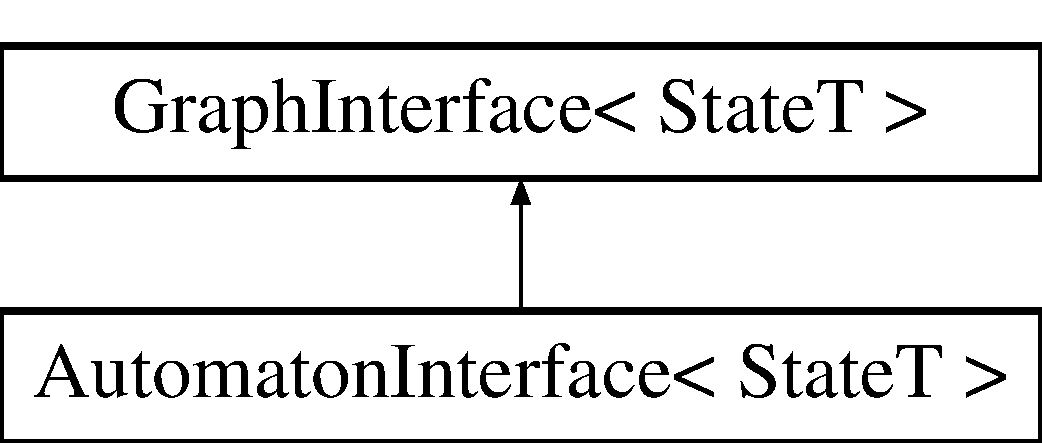
\includegraphics[height=2.000000cm]{classAutomatonInterface}
\end{center}
\end{figure}
\subsection*{\-Public \-Member \-Functions}
\begin{DoxyCompactItemize}
\item 
virtual bool \hyperlink{classAutomatonInterface_a69bfa177f6d048789c828260ff354e42}{is\-Final} (const \-State\-I\-D \-I\-D) const 
\item 
virtual bool \hyperlink{classAutomatonInterface_a97fee6da4d6d64d8ab8afdb57748c6b4}{is\-Initial} (const \-State\-I\-D \-I\-D) const 
\item 
virtual const std\-::vector\*
$<$ \-State\-I\-D $>$ \& \hyperlink{classAutomatonInterface_ad91771a569bbd8fe78b324d3eb28b9f6}{get\-Final\-States} () const 
\item 
virtual const std\-::vector\*
$<$ \-State\-I\-D $>$ \& \hyperlink{classAutomatonInterface_a2674e9b97aa1dd2d975eed682813c8cf}{get\-Initial\-States} () const 
\end{DoxyCompactItemize}
\subsection*{\-Protected \-Attributes}
\begin{DoxyCompactItemize}
\item 
\hypertarget{classAutomatonInterface_a768db02721ec7956749b39457a12327f}{std\-::vector$<$ \-State\-I\-D $>$ \hyperlink{classAutomatonInterface_a768db02721ec7956749b39457a12327f}{initial\-\_\-states}}\label{classAutomatonInterface_a768db02721ec7956749b39457a12327f}

\begin{DoxyCompactList}\small\item\em \-Vector with indexes of initial states (in this case only the first state). \end{DoxyCompactList}\item 
\hypertarget{classAutomatonInterface_a20d4a4c4f51591c2c8c41407162acdaf}{std\-::vector$<$ \-State\-I\-D $>$ \hyperlink{classAutomatonInterface_a20d4a4c4f51591c2c8c41407162acdaf}{final\-\_\-states}}\label{classAutomatonInterface_a20d4a4c4f51591c2c8c41407162acdaf}

\begin{DoxyCompactList}\small\item\em \-Vector with indexes of final states of the \-B\-A. \end{DoxyCompactList}\end{DoxyCompactItemize}
\subsubsection*{template$<$typename \-State\-T$>$ class Automaton\-Interface$<$ State\-T $>$}



\subsection{\-Member \-Function \-Documentation}
\hypertarget{classAutomatonInterface_ad91771a569bbd8fe78b324d3eb28b9f6}{\index{\-Automaton\-Interface@{\-Automaton\-Interface}!get\-Final\-States@{get\-Final\-States}}
\index{get\-Final\-States@{get\-Final\-States}!AutomatonInterface@{\-Automaton\-Interface}}
\subsubsection[{get\-Final\-States}]{\setlength{\rightskip}{0pt plus 5cm}template$<$typename \-State\-T$>$ virtual const std\-::vector$<$\-State\-I\-D$>$\& {\bf \-Automaton\-Interface}$<$ \-State\-T $>$\-::{\bf get\-Final\-States} (
\begin{DoxyParamCaption}
{}
\end{DoxyParamCaption}
) const\hspace{0.3cm}{\ttfamily  \mbox{[}inline, virtual\mbox{]}}}}\label{classAutomatonInterface_ad91771a569bbd8fe78b324d3eb28b9f6}
\-Get \-I\-Ds of all states that are marked as final.

\begin{DoxyReturn}{\-Returns}
vector of final states' \-I\-Ds 
\end{DoxyReturn}
\hypertarget{classAutomatonInterface_a2674e9b97aa1dd2d975eed682813c8cf}{\index{\-Automaton\-Interface@{\-Automaton\-Interface}!get\-Initial\-States@{get\-Initial\-States}}
\index{get\-Initial\-States@{get\-Initial\-States}!AutomatonInterface@{\-Automaton\-Interface}}
\subsubsection[{get\-Initial\-States}]{\setlength{\rightskip}{0pt plus 5cm}template$<$typename \-State\-T$>$ virtual const std\-::vector$<$\-State\-I\-D$>$\& {\bf \-Automaton\-Interface}$<$ \-State\-T $>$\-::{\bf get\-Initial\-States} (
\begin{DoxyParamCaption}
{}
\end{DoxyParamCaption}
) const\hspace{0.3cm}{\ttfamily  \mbox{[}inline, virtual\mbox{]}}}}\label{classAutomatonInterface_a2674e9b97aa1dd2d975eed682813c8cf}
\-Get \-I\-Ds of all states that are marked as initial.

\begin{DoxyReturn}{\-Returns}
vector of initial states' \-I\-Ds 
\end{DoxyReturn}
\hypertarget{classAutomatonInterface_a69bfa177f6d048789c828260ff354e42}{\index{\-Automaton\-Interface@{\-Automaton\-Interface}!is\-Final@{is\-Final}}
\index{is\-Final@{is\-Final}!AutomatonInterface@{\-Automaton\-Interface}}
\subsubsection[{is\-Final}]{\setlength{\rightskip}{0pt plus 5cm}template$<$typename \-State\-T$>$ virtual bool {\bf \-Automaton\-Interface}$<$ \-State\-T $>$\-::{\bf is\-Final} (
\begin{DoxyParamCaption}
\item[{const \-State\-I\-D}]{\-I\-D}
\end{DoxyParamCaption}
) const\hspace{0.3cm}{\ttfamily  \mbox{[}inline, virtual\mbox{]}}}}\label{classAutomatonInterface_a69bfa177f6d048789c828260ff354e42}
\-For a given state find out whether it is marked as final.


\begin{DoxyParams}{\-Parameters}
{\em \-I\-D} & state to test\\
\hline
\end{DoxyParams}
\begin{DoxyReturn}{\-Returns}
true if the state is final 
\end{DoxyReturn}
\hypertarget{classAutomatonInterface_a97fee6da4d6d64d8ab8afdb57748c6b4}{\index{\-Automaton\-Interface@{\-Automaton\-Interface}!is\-Initial@{is\-Initial}}
\index{is\-Initial@{is\-Initial}!AutomatonInterface@{\-Automaton\-Interface}}
\subsubsection[{is\-Initial}]{\setlength{\rightskip}{0pt plus 5cm}template$<$typename \-State\-T$>$ virtual bool {\bf \-Automaton\-Interface}$<$ \-State\-T $>$\-::{\bf is\-Initial} (
\begin{DoxyParamCaption}
\item[{const \-State\-I\-D}]{\-I\-D}
\end{DoxyParamCaption}
) const\hspace{0.3cm}{\ttfamily  \mbox{[}inline, virtual\mbox{]}}}}\label{classAutomatonInterface_a97fee6da4d6d64d8ab8afdb57748c6b4}
\-For given state find out if it is marked as initial.


\begin{DoxyParams}{\-Parameters}
{\em \-I\-D} & state to test\\
\hline
\end{DoxyParams}
\begin{DoxyReturn}{\-Returns}
true if the state is initial 
\end{DoxyReturn}


\-The documentation for this class was generated from the following file\-:\begin{DoxyCompactItemize}
\item 
construction/automaton\-\_\-interface.\-hpp\end{DoxyCompactItemize}

\hypertarget{classAutomatonParser}{\section{\-Automaton\-Parser \-Class \-Reference}
\label{classAutomatonParser}\index{\-Automaton\-Parser@{\-Automaton\-Parser}}
}


\-This object is responsible for parsing and translation of data related to the tested property.  




{\ttfamily \#include $<$automaton\-\_\-parser.\-hpp$>$}

\subsection*{\-Public \-Member \-Functions}
\begin{DoxyCompactItemize}
\item 
\hypertarget{classAutomatonParser_a6f1b416fa12046eacb977f38d0be12cc}{\hyperlink{classAutomatonParser_a6f1b416fa12046eacb977f38d0be12cc}{\-Automaton\-Parser} (\hyperlink{classModel}{\-Model} \&\-\_\-model)}\label{classAutomatonParser_a6f1b416fa12046eacb977f38d0be12cc}

\begin{DoxyCompactList}\small\item\em \-Simple constructor, passes references. \end{DoxyCompactList}\item 
void \hyperlink{classAutomatonParser_a9a4a3202f693f351a88ada8dbf7852db}{parse} (const rapidxml\-::xml\-\_\-node$<$$>$ $\ast$const model\-\_\-node)
\end{DoxyCompactItemize}


\subsection{\-Member \-Function \-Documentation}
\hypertarget{classAutomatonParser_a9a4a3202f693f351a88ada8dbf7852db}{\index{\-Automaton\-Parser@{\-Automaton\-Parser}!parse@{parse}}
\index{parse@{parse}!AutomatonParser@{\-Automaton\-Parser}}
\subsubsection[{parse}]{\setlength{\rightskip}{0pt plus 5cm}void {\bf \-Automaton\-Parser\-::parse} (
\begin{DoxyParamCaption}
\item[{const rapidxml\-::xml\-\_\-node$<$$>$ $\ast$const}]{model\-\_\-node}
\end{DoxyParamCaption}
)\hspace{0.3cm}{\ttfamily  \mbox{[}inline\mbox{]}}}}\label{classAutomatonParser_a9a4a3202f693f351a88ada8dbf7852db}
\-Main parsing function. \-It expects a pointer to inside of a \-M\-O\-D\-E\-L node. 

\-The documentation for this class was generated from the following file\-:\begin{DoxyCompactItemize}
\item 
parsing/automaton\-\_\-parser.\-hpp\end{DoxyCompactItemize}

\hypertarget{structAutomatonStateProperty}{\section{\-Automaton\-State\-Property$<$ \-Transition $>$ \-Struct \-Template \-Reference}
\label{structAutomatonStateProperty}\index{\-Automaton\-State\-Property$<$ Transition $>$@{\-Automaton\-State\-Property$<$ Transition $>$}}
}


\-A state structure enhanced with information whether the state is final and/or initial.  




{\ttfamily \#include $<$automaton\-\_\-interface.\-hpp$>$}

\-Inheritance diagram for \-Automaton\-State\-Property$<$ \-Transition $>$\-:\begin{figure}[H]
\begin{center}
\leavevmode
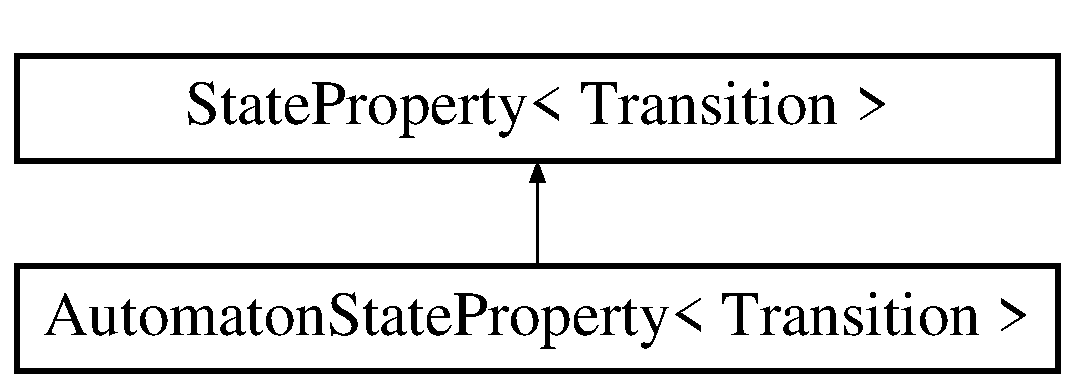
\includegraphics[height=2.000000cm]{structAutomatonStateProperty}
\end{center}
\end{figure}
\subsection*{\-Public \-Member \-Functions}
\begin{DoxyCompactItemize}
\item 
\hyperlink{structAutomatonStateProperty_aefba38decd169cc6177e59cd9bce67d0}{\-Automaton\-State\-Property} (const bool \-\_\-initial, const bool \-\_\-final, const \-State\-I\-D \hyperlink{structStateProperty_af33be20c9033f9b6524c0447e7ac647e}{\-I\-D}, const std\-::string \&\&\hyperlink{structStateProperty_a7cfb634f80b68196eefa54e8ee98a5fe}{label})
\end{DoxyCompactItemize}
\subsection*{\-Public \-Attributes}
\begin{DoxyCompactItemize}
\item 
\hypertarget{structAutomatonStateProperty_a01c05b93d68d3f72b76ab9835abc5476}{bool \hyperlink{structAutomatonStateProperty_a01c05b93d68d3f72b76ab9835abc5476}{initial}}\label{structAutomatonStateProperty_a01c05b93d68d3f72b76ab9835abc5476}

\begin{DoxyCompactList}\small\item\em \-True if the state is initial. \end{DoxyCompactList}\item 
\hypertarget{structAutomatonStateProperty_aa95898834a149d202575a6f655a5e5e2}{bool \hyperlink{structAutomatonStateProperty_aa95898834a149d202575a6f655a5e5e2}{final}}\label{structAutomatonStateProperty_aa95898834a149d202575a6f655a5e5e2}

\begin{DoxyCompactList}\small\item\em \-True if this state is final. \end{DoxyCompactList}\end{DoxyCompactItemize}
\subsubsection*{template$<$typename \-Transition$>$ struct Automaton\-State\-Property$<$ Transition $>$}



\subsection{\-Constructor \& \-Destructor \-Documentation}
\hypertarget{structAutomatonStateProperty_aefba38decd169cc6177e59cd9bce67d0}{\index{\-Automaton\-State\-Property@{\-Automaton\-State\-Property}!\-Automaton\-State\-Property@{\-Automaton\-State\-Property}}
\index{\-Automaton\-State\-Property@{\-Automaton\-State\-Property}!AutomatonStateProperty@{\-Automaton\-State\-Property}}
\subsubsection[{\-Automaton\-State\-Property}]{\setlength{\rightskip}{0pt plus 5cm}template$<$typename \-Transition$>$ {\bf \-Automaton\-State\-Property}$<$ \-Transition $>$\-::{\bf \-Automaton\-State\-Property} (
\begin{DoxyParamCaption}
\item[{const bool}]{\-\_\-initial, }
\item[{const bool}]{\-\_\-final, }
\item[{const \-State\-I\-D}]{\-I\-D, }
\item[{const std\-::string \&\&}]{label}
\end{DoxyParamCaption}
)\hspace{0.3cm}{\ttfamily  \mbox{[}inline\mbox{]}}}}\label{structAutomatonStateProperty_aefba38decd169cc6177e59cd9bce67d0}
\-Adds information if the state is final or initial, passes the rest. 

\-The documentation for this struct was generated from the following file\-:\begin{DoxyCompactItemize}
\item 
construction/automaton\-\_\-interface.\-hpp\end{DoxyCompactItemize}

\hypertarget{classAutomatonStructure}{\section{\-Automaton\-Structure \-Class \-Reference}
\label{classAutomatonStructure}\index{\-Automaton\-Structure@{\-Automaton\-Structure}}
}


\-A \-Buchi automaton designed to control some $\omega$-\/regular property.  




{\ttfamily \#include $<$automaton\-\_\-structure.\-hpp$>$}

\-Inheritance diagram for \-Automaton\-Structure\-:\begin{figure}[H]
\begin{center}
\leavevmode
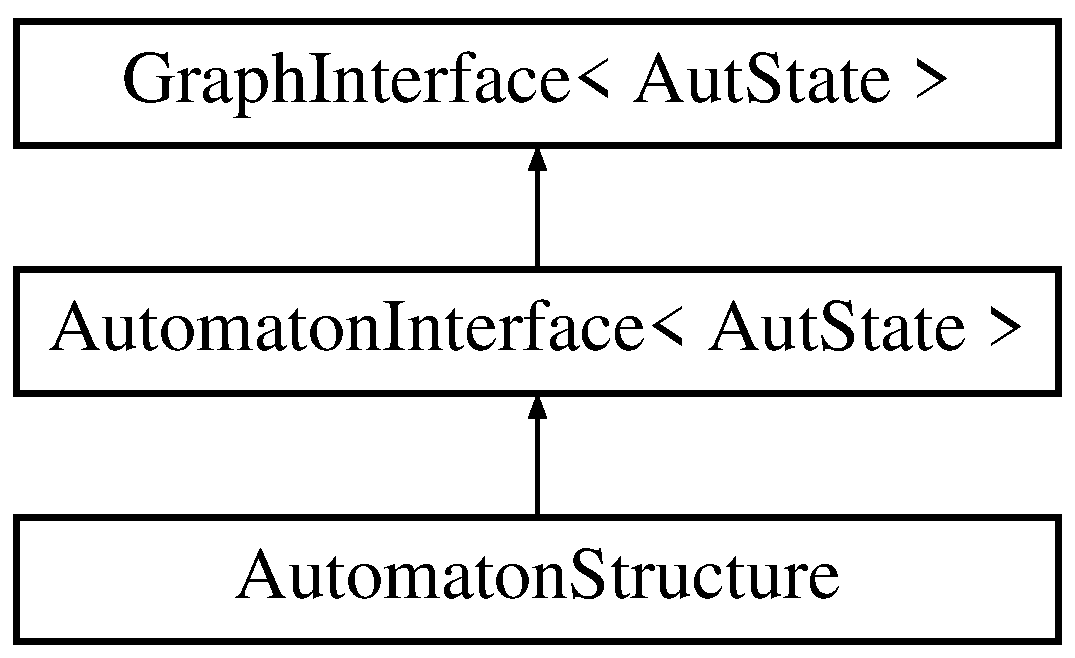
\includegraphics[height=3.000000cm]{classAutomatonStructure}
\end{center}
\end{figure}
\subsection*{\-Public \-Member \-Functions}
\begin{DoxyCompactItemize}
\item 
\hypertarget{classAutomatonStructure_a71e2f5d77f0118e9fc0dbaeb5024b9a1}{\hyperlink{classAutomatonStructure_a71e2f5d77f0118e9fc0dbaeb5024b9a1}{\-Automaton\-Structure} ()}\label{classAutomatonStructure_a71e2f5d77f0118e9fc0dbaeb5024b9a1}

\begin{DoxyCompactList}\small\item\em \-Default empty constructor. \end{DoxyCompactList}\item 
bool \hyperlink{classAutomatonStructure_a3075f9c11cb21b6bab25854bac866eea}{is\-Transition\-Feasible} (const \-State\-I\-D \-I\-D, const std\-::size\-\_\-t transition\-\_\-num, const \-Levels \&levels) const 
\end{DoxyCompactItemize}
\subsection*{\-Friends}
\begin{DoxyCompactItemize}
\item 
\hypertarget{classAutomatonStructure_aa8c70fdebc72ce387f4c6dbf6291f149}{class {\bfseries \-Automaton\-Builder}}\label{classAutomatonStructure_aa8c70fdebc72ce387f4c6dbf6291f149}

\end{DoxyCompactItemize}


\subsection{\-Detailed \-Description}
\hyperlink{classAutomatonStructure}{\-Automaton\-Structure} stores \-Buchi automaton with edges labelled by values the \-K\-S can be in for the transition to be allowed. \hyperlink{classAutomatonStructure}{\-Automaton\-Structure} data can be set only from the \-Automaton\-Structure\-Builder object. 

\subsection{\-Member \-Function \-Documentation}
\hypertarget{classAutomatonStructure_a3075f9c11cb21b6bab25854bac866eea}{\index{\-Automaton\-Structure@{\-Automaton\-Structure}!is\-Transition\-Feasible@{is\-Transition\-Feasible}}
\index{is\-Transition\-Feasible@{is\-Transition\-Feasible}!AutomatonStructure@{\-Automaton\-Structure}}
\subsubsection[{is\-Transition\-Feasible}]{\setlength{\rightskip}{0pt plus 5cm}bool {\bf \-Automaton\-Structure\-::is\-Transition\-Feasible} (
\begin{DoxyParamCaption}
\item[{const \-State\-I\-D}]{\-I\-D, }
\item[{const std\-::size\-\_\-t}]{transition\-\_\-num, }
\item[{const \-Levels \&}]{levels}
\end{DoxyParamCaption}
) const\hspace{0.3cm}{\ttfamily  \mbox{[}inline\mbox{]}}}}\label{classAutomatonStructure_a3075f9c11cb21b6bab25854bac866eea}
\-Checks if a transition of the \-B\-A is possible in the current state of a \-K\-S.


\begin{DoxyParams}{\-Parameters}
{\em \-I\-D} & source state of the transition \\
\hline
{\em transition\-\_\-num} & ordinal number of the transition \\
\hline
{\em levels} & current levels of species i.\-e. the state of the \-K\-S\\
\hline
\end{DoxyParams}
\begin{DoxyReturn}{\-Returns}
true if the transition is feasible 
\end{DoxyReturn}


\-The documentation for this class was generated from the following file\-:\begin{DoxyCompactItemize}
\item 
construction/automaton\-\_\-structure.\-hpp\end{DoxyCompactItemize}

\hypertarget{structAutState}{\section{\-Aut\-State \-Struct \-Reference}
\label{structAutState}\index{\-Aut\-State@{\-Aut\-State}}
}


\-Storing a single state of the \-Buchi automaton. \-This state is extended with a value saying wheter the states is final.  




{\ttfamily \#include $<$automaton\-\_\-structure.\-hpp$>$}

\-Inheritance diagram for \-Aut\-State\-:\begin{figure}[H]
\begin{center}
\leavevmode
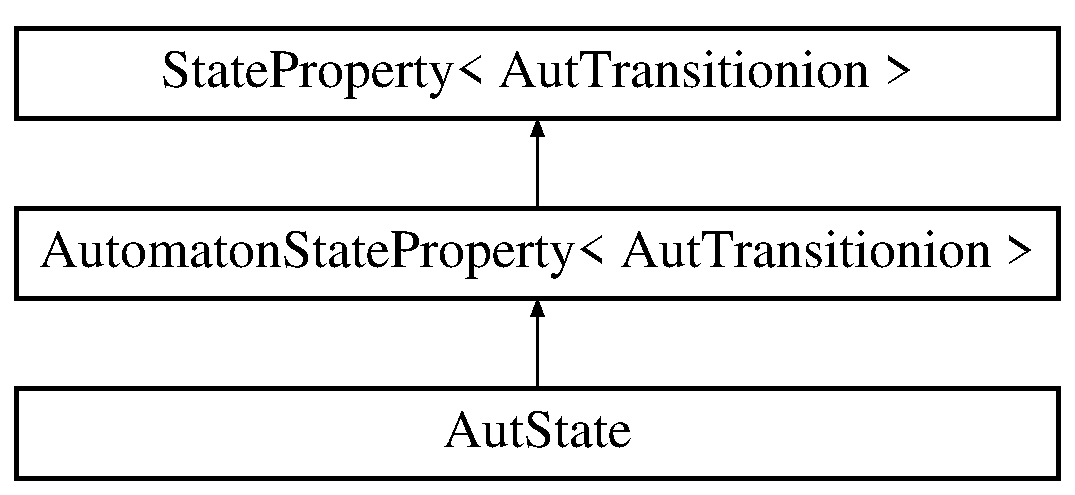
\includegraphics[height=3.000000cm]{structAutState}
\end{center}
\end{figure}
\subsection*{\-Public \-Member \-Functions}
\begin{DoxyCompactItemize}
\item 
\hypertarget{structAutState_a6cc8e67981514be7120c2e4963e63ee6}{\hyperlink{structAutState_a6cc8e67981514be7120c2e4963e63ee6}{\-Aut\-State} (const \-State\-I\-D \hyperlink{structStateProperty_af33be20c9033f9b6524c0447e7ac647e}{\-I\-D}, const bool \hyperlink{structAutomatonStateProperty_aa95898834a149d202575a6f655a5e5e2}{final}, std\-::string \&\&\hyperlink{structStateProperty_a7cfb634f80b68196eefa54e8ee98a5fe}{label})}\label{structAutState_a6cc8e67981514be7120c2e4963e63ee6}

\begin{DoxyCompactList}\small\item\em \-Fills data and checks if the state has value -\/$>$ is initial. \end{DoxyCompactList}\end{DoxyCompactItemize}


\-The documentation for this struct was generated from the following file\-:\begin{DoxyCompactItemize}
\item 
construction/automaton\-\_\-structure.\-hpp\end{DoxyCompactItemize}

\hypertarget{structAutTransitionion}{\section{\-Aut\-Transitionion \-Struct \-Reference}
\label{structAutTransitionion}\index{\-Aut\-Transitionion@{\-Aut\-Transitionion}}
}


\-Single labelled transition from one state to another.  




{\ttfamily \#include $<$automaton\-\_\-structure.\-hpp$>$}

\-Inheritance diagram for \-Aut\-Transitionion\-:\begin{figure}[H]
\begin{center}
\leavevmode
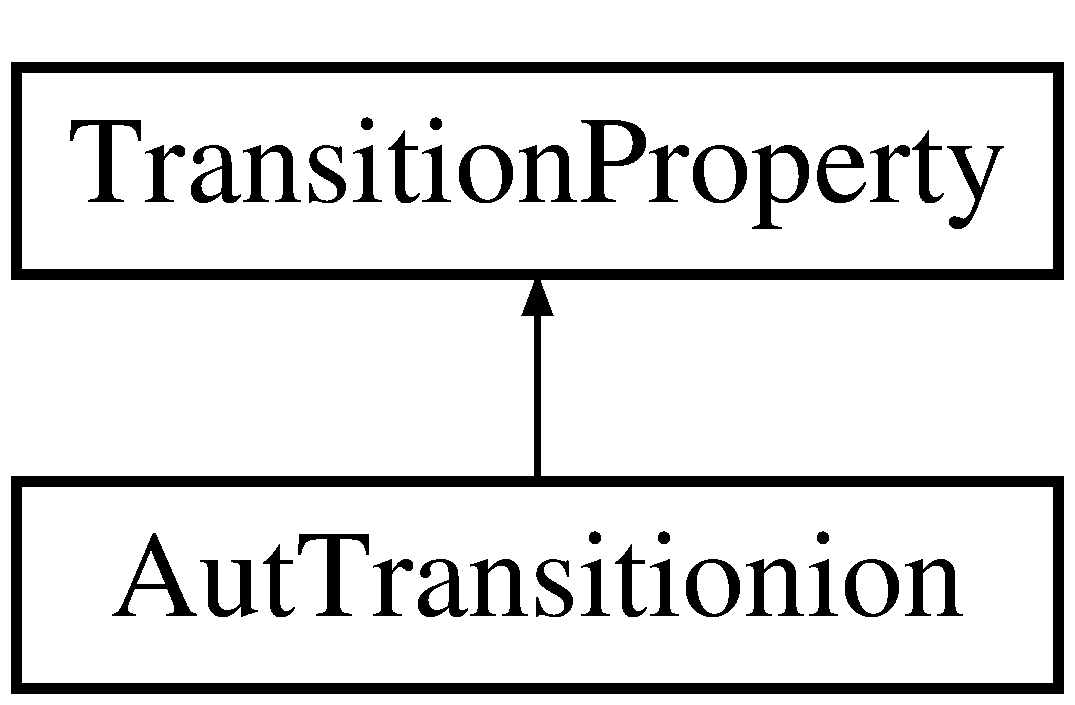
\includegraphics[height=2.000000cm]{structAutTransitionion}
\end{center}
\end{figure}
\subsection*{\-Public \-Member \-Functions}
\begin{DoxyCompactItemize}
\item 
\hypertarget{structAutTransitionion_a8ffa8981f3dc8cd2de51674fb5937828}{\hyperlink{structAutTransitionion_a8ffa8981f3dc8cd2de51674fb5937828}{\-Aut\-Transitionion} (const \-State\-I\-D \hyperlink{structTransitionProperty_a1e272cf5a26a0db442ac0fed5b797386}{target\-\_\-\-I\-D}, \-Allowed\-Values \&\&\-\_\-allowed\-\_\-values)}\label{structAutTransitionion_a8ffa8981f3dc8cd2de51674fb5937828}

\begin{DoxyCompactList}\small\item\em \-Simple filler, assigns values to all the variables. \end{DoxyCompactList}\end{DoxyCompactItemize}
\subsection*{\-Public \-Attributes}
\begin{DoxyCompactItemize}
\item 
\hypertarget{structAutTransitionion_a17e3d0000118d6464369ac61faf1d40e}{\-Allowed\-Values \hyperlink{structAutTransitionion_a17e3d0000118d6464369ac61faf1d40e}{allowed\-\_\-values}}\label{structAutTransitionion_a17e3d0000118d6464369ac61faf1d40e}

\begin{DoxyCompactList}\small\item\em \-Allowed values of species for this transition. \end{DoxyCompactList}\end{DoxyCompactItemize}


\-The documentation for this struct was generated from the following file\-:\begin{DoxyCompactItemize}
\item 
construction/automaton\-\_\-structure.\-hpp\end{DoxyCompactItemize}

\hypertarget{classBasicStructure}{\section{\-Basic\-Structure \-Class \-Reference}
\label{classBasicStructure}\index{\-Basic\-Structure@{\-Basic\-Structure}}
}


\-A simple structure describing the complete state space.  




{\ttfamily \#include $<$basic\-\_\-structure.\-hpp$>$}

\-Inheritance diagram for \-Basic\-Structure\-:\begin{figure}[H]
\begin{center}
\leavevmode
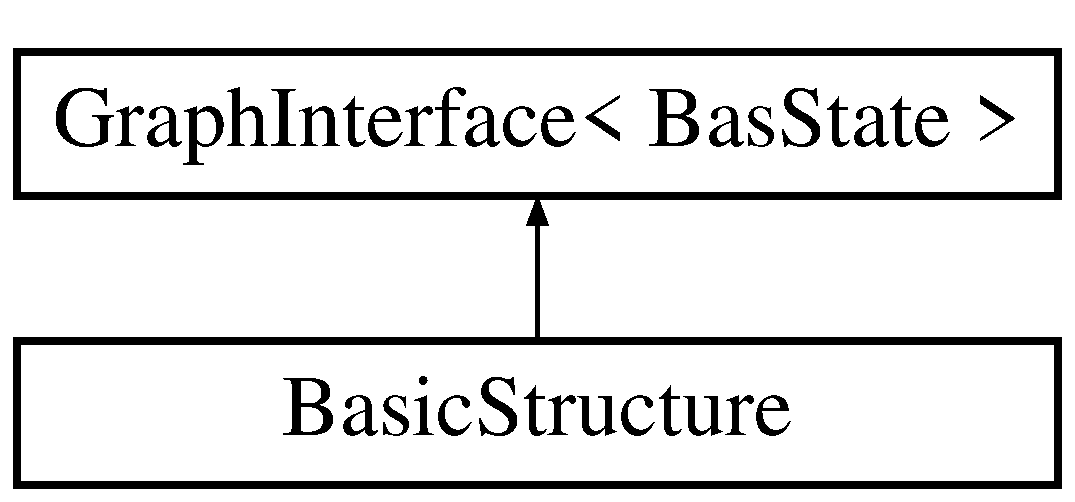
\includegraphics[height=2.000000cm]{classBasicStructure}
\end{center}
\end{figure}
\subsection*{\-Public \-Member \-Functions}
\begin{DoxyCompactItemize}
\item 
\hypertarget{classBasicStructure_ae2069c7d1d75da4f17093dc50aa35c8c}{\hyperlink{classBasicStructure_ae2069c7d1d75da4f17093dc50aa35c8c}{\-Basic\-Structure} ()}\label{classBasicStructure_ae2069c7d1d75da4f17093dc50aa35c8c}

\begin{DoxyCompactList}\small\item\em \-Default empty constructor, needed to create an empty object that will be filled. \end{DoxyCompactList}\item 
const \-Levels \& \hyperlink{classBasicStructure_a16e4995e8983e3882015158ef3141dba}{get\-State\-Levels} (const \-State\-I\-D \-I\-D) const 
\item 
std\-::size\-\_\-t \hyperlink{classBasicStructure_abba9142ad864c119a657a7c4ea84e074}{get\-Specie\-I\-D} (const \-State\-I\-D \-I\-D, const std\-::size\-\_\-t neighbour\-\_\-index) const 
\item 
\-Direction \hyperlink{classBasicStructure_af6bd4e6df2c4fee49d372bc9455543ac}{get\-Direction} (const \-State\-I\-D \-I\-D, const std\-::size\-\_\-t neighbour\-\_\-index) const 
\end{DoxyCompactItemize}
\subsection*{\-Friends}
\begin{DoxyCompactItemize}
\item 
\hypertarget{classBasicStructure_ad482d25720baca819f24eed850bd41e2}{class {\bfseries \-Basic\-Structure\-Builder}}\label{classBasicStructure_ad482d25720baca819f24eed850bd41e2}

\end{DoxyCompactItemize}


\subsection{\-Detailed \-Description}
\hyperlink{classBasicStructure}{\-Basic\-Structure} stores states of the \-Kripke structure created from the model -\/ each state knows its levels and indexes of all the neighbours. \-Order of neighbours of state is (specie 1 down, specie 1 stay, specie 1 up, specie 2 down, ... ) \hyperlink{classBasicStructure}{\-Basic\-Structure} data can be set only form the \hyperlink{classBasicStructureBuilder}{\-Basic\-Structure\-Builder} object. 

\subsection{\-Member \-Function \-Documentation}
\hypertarget{classBasicStructure_af6bd4e6df2c4fee49d372bc9455543ac}{\index{\-Basic\-Structure@{\-Basic\-Structure}!get\-Direction@{get\-Direction}}
\index{get\-Direction@{get\-Direction}!BasicStructure@{\-Basic\-Structure}}
\subsubsection[{get\-Direction}]{\setlength{\rightskip}{0pt plus 5cm}\-Direction {\bf \-Basic\-Structure\-::get\-Direction} (
\begin{DoxyParamCaption}
\item[{const \-State\-I\-D}]{\-I\-D, }
\item[{const std\-::size\-\_\-t}]{neighbour\-\_\-index}
\end{DoxyParamCaption}
) const\hspace{0.3cm}{\ttfamily  \mbox{[}inline\mbox{]}}}}\label{classBasicStructure_af6bd4e6df2c4fee49d372bc9455543ac}

\begin{DoxyParams}{\-Parameters}
{\em \-I\-D} & \-I\-D of the state to get the neighbour from \\
\hline
{\em neighbour\-\_\-index} & index in the vector of neighbours\\
\hline
\end{DoxyParams}
\begin{DoxyReturn}{\-Returns}
\-Direction in which the specie changes 
\end{DoxyReturn}
\hypertarget{classBasicStructure_abba9142ad864c119a657a7c4ea84e074}{\index{\-Basic\-Structure@{\-Basic\-Structure}!get\-Specie\-I\-D@{get\-Specie\-I\-D}}
\index{get\-Specie\-I\-D@{get\-Specie\-I\-D}!BasicStructure@{\-Basic\-Structure}}
\subsubsection[{get\-Specie\-I\-D}]{\setlength{\rightskip}{0pt plus 5cm}std\-::size\-\_\-t {\bf \-Basic\-Structure\-::get\-Specie\-I\-D} (
\begin{DoxyParamCaption}
\item[{const \-State\-I\-D}]{\-I\-D, }
\item[{const std\-::size\-\_\-t}]{neighbour\-\_\-index}
\end{DoxyParamCaption}
) const\hspace{0.3cm}{\ttfamily  \mbox{[}inline\mbox{]}}}}\label{classBasicStructure_abba9142ad864c119a657a7c4ea84e074}

\begin{DoxyParams}{\-Parameters}
{\em \-I\-D} & \-I\-D of the state to get the neighbour from \\
\hline
{\em neighbour\-\_\-index} & index in the vector of neighbours\\
\hline
\end{DoxyParams}
\begin{DoxyReturn}{\-Returns}
\-I\-D of the specie that vary between the two states 
\end{DoxyReturn}
\hypertarget{classBasicStructure_a16e4995e8983e3882015158ef3141dba}{\index{\-Basic\-Structure@{\-Basic\-Structure}!get\-State\-Levels@{get\-State\-Levels}}
\index{get\-State\-Levels@{get\-State\-Levels}!BasicStructure@{\-Basic\-Structure}}
\subsubsection[{get\-State\-Levels}]{\setlength{\rightskip}{0pt plus 5cm}const \-Levels\& {\bf \-Basic\-Structure\-::get\-State\-Levels} (
\begin{DoxyParamCaption}
\item[{const \-State\-I\-D}]{\-I\-D}
\end{DoxyParamCaption}
) const\hspace{0.3cm}{\ttfamily  \mbox{[}inline\mbox{]}}}}\label{classBasicStructure_a16e4995e8983e3882015158ef3141dba}

\begin{DoxyParams}{\-Parameters}
{\em \-I\-D} & \-I\-D of the state to get\\
\hline
\end{DoxyParams}
\begin{DoxyReturn}{\-Returns}
levels of the state 
\end{DoxyReturn}


\-The documentation for this class was generated from the following file\-:\begin{DoxyCompactItemize}
\item 
construction/basic\-\_\-structure.\-hpp\end{DoxyCompactItemize}

\hypertarget{classBasicStructureBuilder}{\section{\-Basic\-Structure\-Builder \-Class \-Reference}
\label{classBasicStructureBuilder}\index{\-Basic\-Structure\-Builder@{\-Basic\-Structure\-Builder}}
}


\-Creates a full state space as a simple graph as a \hyperlink{classBasicStructure}{\-Basic\-Structure} object.  




{\ttfamily \#include $<$basic\-\_\-structure\-\_\-builder.\-hpp$>$}

\subsection*{\-Public \-Member \-Functions}
\begin{DoxyCompactItemize}
\item 
\hyperlink{classBasicStructureBuilder_ab5143ea3bfccc2afa3f348a0bb2cb3fe}{\-Basic\-Structure\-Builder} (const \hyperlink{classModel}{\-Model} \&\-\_\-model, \hyperlink{classBasicStructure}{\-Basic\-Structure} \&\-\_\-structure)
\item 
void \hyperlink{classBasicStructureBuilder_a71a0c391b82ca2d4fd3bac50a8589823}{build\-Structure} ()
\end{DoxyCompactItemize}


\subsection{\-Detailed \-Description}
\hyperlink{classBasicStructureBuilder}{\-Basic\-Structure\-Builder} creates the \hyperlink{classBasicStructure}{\-Basic\-Structure} (\-Simple \-Kripke \-Structure) from the model data. \-In each iteration of the creation, a new state is generated as a cartesian product of values of the species. \-All the combinations are used. \-Each state is provided with indexes of their neighbours. \-For each dimension (specie) there are three neighbours, if possible, base on the change of the specie's value -\/ up, stay or down. 

\subsection{\-Constructor \& \-Destructor \-Documentation}
\hypertarget{classBasicStructureBuilder_ab5143ea3bfccc2afa3f348a0bb2cb3fe}{\index{\-Basic\-Structure\-Builder@{\-Basic\-Structure\-Builder}!\-Basic\-Structure\-Builder@{\-Basic\-Structure\-Builder}}
\index{\-Basic\-Structure\-Builder@{\-Basic\-Structure\-Builder}!BasicStructureBuilder@{\-Basic\-Structure\-Builder}}
\subsubsection[{\-Basic\-Structure\-Builder}]{\setlength{\rightskip}{0pt plus 5cm}\-Basic\-Structure\-Builder\-::\-Basic\-Structure\-Builder (
\begin{DoxyParamCaption}
\item[{const {\bf \-Model} \&}]{\-\_\-model, }
\item[{{\bf \-Basic\-Structure} \&}]{\-\_\-structure}
\end{DoxyParamCaption}
)\hspace{0.3cm}{\ttfamily  \mbox{[}inline\mbox{]}}}}\label{classBasicStructureBuilder_ab5143ea3bfccc2afa3f348a0bb2cb3fe}
\-Constructor initializes basic information from the model 

\subsection{\-Member \-Function \-Documentation}
\hypertarget{classBasicStructureBuilder_a71a0c391b82ca2d4fd3bac50a8589823}{\index{\-Basic\-Structure\-Builder@{\-Basic\-Structure\-Builder}!build\-Structure@{build\-Structure}}
\index{build\-Structure@{build\-Structure}!BasicStructureBuilder@{\-Basic\-Structure\-Builder}}
\subsubsection[{build\-Structure}]{\setlength{\rightskip}{0pt plus 5cm}void {\bf \-Basic\-Structure\-Builder\-::build\-Structure} (
\begin{DoxyParamCaption}
{}
\end{DoxyParamCaption}
)\hspace{0.3cm}{\ttfamily  \mbox{[}inline\mbox{]}}}}\label{classBasicStructureBuilder_a71a0c391b82ca2d4fd3bac50a8589823}
\-Create the states from the model and fill the structure with them. 

\-The documentation for this class was generated from the following file\-:\begin{DoxyCompactItemize}
\item 
construction/basic\-\_\-structure\-\_\-builder.\-hpp\end{DoxyCompactItemize}

\hypertarget{structBasState}{\section{\-Bas\-State \-Struct \-Reference}
\label{structBasState}\index{\-Bas\-State@{\-Bas\-State}}
}


\-Storing a single state -\/ its activation levels of each of the species and \-I\-Ds of states that are neighbours (differ only in single step of single value).  




{\ttfamily \#include $<$basic\-\_\-structure.\-hpp$>$}

\-Inheritance diagram for \-Bas\-State\-:\begin{figure}[H]
\begin{center}
\leavevmode
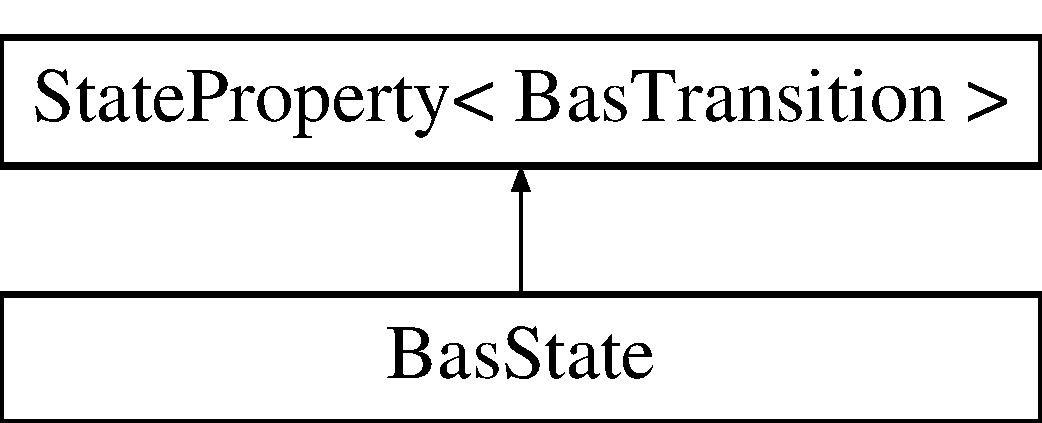
\includegraphics[height=2.000000cm]{structBasState}
\end{center}
\end{figure}
\subsection*{\-Public \-Member \-Functions}
\begin{DoxyCompactItemize}
\item 
\hypertarget{structBasState_acd4aaaa80478736104c7473a1b0f9285}{\hyperlink{structBasState_acd4aaaa80478736104c7473a1b0f9285}{\-Bas\-State} (const \-State\-I\-D \hyperlink{structStateProperty_af33be20c9033f9b6524c0447e7ac647e}{\-I\-D}, const \-Levels \-\_\-species\-\_\-level, const std\-::string \&\&\hyperlink{structStateProperty_a7cfb634f80b68196eefa54e8ee98a5fe}{label})}\label{structBasState_acd4aaaa80478736104c7473a1b0f9285}

\begin{DoxyCompactList}\small\item\em \-Simple filler, assigns values to all the variables. \end{DoxyCompactList}\end{DoxyCompactItemize}
\subsection*{\-Public \-Attributes}
\begin{DoxyCompactItemize}
\item 
\hypertarget{structBasState_afeedce916ea0dc756525f0f38ec8049b}{\-Levels \hyperlink{structBasState_afeedce916ea0dc756525f0f38ec8049b}{species\-\_\-level}}\label{structBasState_afeedce916ea0dc756525f0f38ec8049b}

\begin{DoxyCompactList}\small\item\em \-Species\-\_\-level\mbox{[}i\mbox{]} = activation level of specie i. \end{DoxyCompactList}\end{DoxyCompactItemize}


\-The documentation for this struct was generated from the following file\-:\begin{DoxyCompactItemize}
\item 
construction/basic\-\_\-structure.\-hpp\end{DoxyCompactItemize}

\hypertarget{structBasTransition}{\section{\-Bas\-Transition \-Struct \-Reference}
\label{structBasTransition}\index{\-Bas\-Transition@{\-Bas\-Transition}}
}


\-Stores an unlabelled transition to next state.  




{\ttfamily \#include $<$basic\-\_\-structure.\-hpp$>$}

\-Inheritance diagram for \-Bas\-Transition\-:\begin{figure}[H]
\begin{center}
\leavevmode
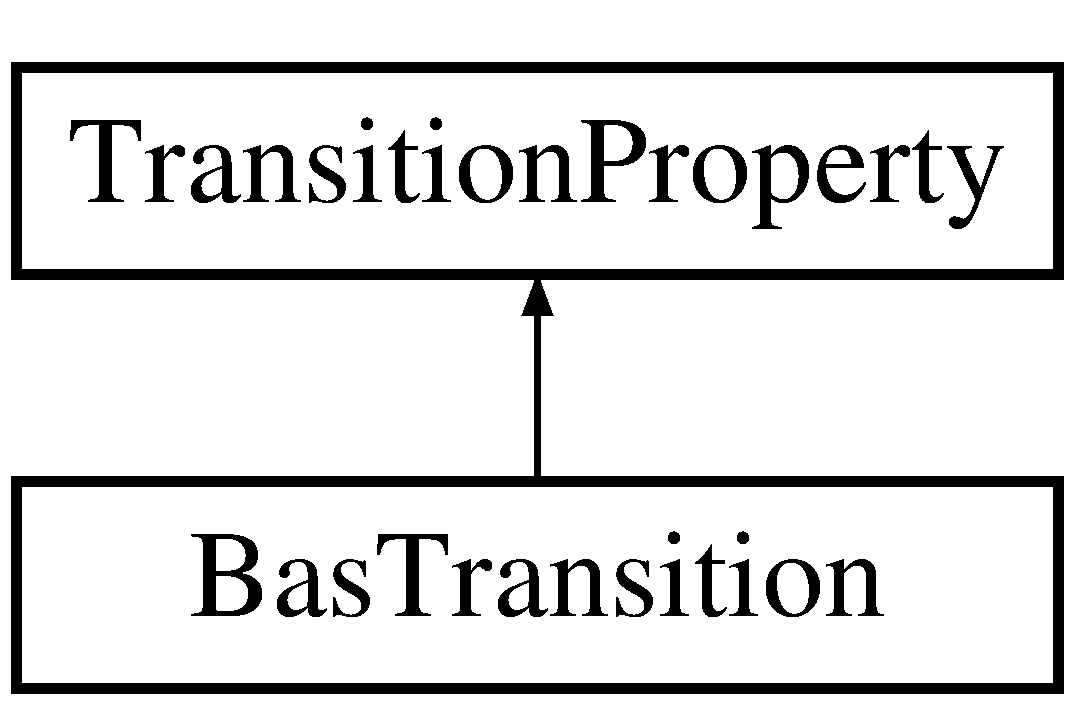
\includegraphics[height=2.000000cm]{structBasTransition}
\end{center}
\end{figure}
\subsection*{\-Public \-Member \-Functions}
\begin{DoxyCompactItemize}
\item 
\hypertarget{structBasTransition_a429dac2adbd7ac5ce7d0c3c6a716d54e}{\hyperlink{structBasTransition_a429dac2adbd7ac5ce7d0c3c6a716d54e}{\-Bas\-Transition} (const \-State\-I\-D \hyperlink{structTransitionProperty_a1e272cf5a26a0db442ac0fed5b797386}{target\-\_\-\-I\-D}, const std\-::size\-\_\-t \-\_\-changed\-\_\-specie, const \-Direction \-\_\-change\-\_\-direction)}\label{structBasTransition_a429dac2adbd7ac5ce7d0c3c6a716d54e}

\begin{DoxyCompactList}\small\item\em \-Simple filler, assigns values to all the variables. \end{DoxyCompactList}\end{DoxyCompactItemize}
\subsection*{\-Public \-Attributes}
\begin{DoxyCompactItemize}
\item 
\hypertarget{structBasTransition_abc640fc68f846a5f4c328cf801b3b451}{std\-::size\-\_\-t \hyperlink{structBasTransition_abc640fc68f846a5f4c328cf801b3b451}{changed\-\_\-specie}}\label{structBasTransition_abc640fc68f846a5f4c328cf801b3b451}

\begin{DoxyCompactList}\small\item\em \-I\-D of specie that differs between this and neighbour. \end{DoxyCompactList}\item 
\hypertarget{structBasTransition_a88ce704d3a9549dbe5c179084b66f541}{\-Direction \hyperlink{structBasTransition_a88ce704d3a9549dbe5c179084b66f541}{change\-\_\-direction}}\label{structBasTransition_a88ce704d3a9549dbe5c179084b66f541}

\begin{DoxyCompactList}\small\item\em \-Way the specie's value is changed. \end{DoxyCompactList}\end{DoxyCompactItemize}


\-The documentation for this struct was generated from the following file\-:\begin{DoxyCompactItemize}
\item 
construction/basic\-\_\-structure.\-hpp\end{DoxyCompactItemize}

\hypertarget{classColoringAnalyzer}{\section{\-Coloring\-Analyzer \-Class \-Reference}
\label{classColoringAnalyzer}\index{\-Coloring\-Analyzer@{\-Coloring\-Analyzer}}
}


\-A storage of individual final states together with their coloring and to further provide necessary data for the output as requested.  




{\ttfamily \#include $<$coloring\-\_\-analyzer.\-hpp$>$}

\subsection*{\-Public \-Member \-Functions}
\begin{DoxyCompactItemize}
\item 
const std\-::vector$<$ std\-::string $>$ \hyperlink{classColoringAnalyzer_ac0fff9753064754b7966c48f2cae7aee}{get\-Output} () const 
\item 
const std\-::vector$<$ std\-::string $>$ \hyperlink{classColoringAnalyzer_ac4c6f413fb0f55f5861ffdd12a9380d7}{get\-Strings} (const \-State\-I\-D \-I\-D) const 
\item 
const std\-::vector$<$ std\-::string $>$ \hyperlink{classColoringAnalyzer_a0300b8f6477ca1c8b0abc936e6ed2837}{get\-Strings} () const 
\item 
const std\-::vector$<$ \-Color\-Num $>$ \hyperlink{classColoringAnalyzer_af99abef2a9541c6346fee2965f4dc0b6}{get\-Numbers} (const \-State\-I\-D \-I\-D) const 
\item 
const std\-::vector$<$ \-Color\-Num $>$ \hyperlink{classColoringAnalyzer_a97cf3d6513f903b8ea0c115c7e2961b6}{get\-Numbers} () const 
\item 
\-Paramset \hyperlink{classColoringAnalyzer_a64e77cbc80b792ce5f4f06d1dedd6c31}{get\-Mask} (const \-State\-I\-D \-I\-D) const 
\item 
\-Paramset \hyperlink{classColoringAnalyzer_a4f1587d869c8ca167d7261e9deed290d}{get\-Mask} () const 
\end{DoxyCompactItemize}
\subsection*{\-Friends}
\begin{DoxyCompactItemize}
\item 
\hypertarget{classColoringAnalyzer_a1d08da922bb492eb0ec8123e88cbecb5}{class {\bfseries \-Synthesis\-Manager}}\label{classColoringAnalyzer_a1d08da922bb492eb0ec8123e88cbecb5}

\end{DoxyCompactItemize}


\subsection{\-Member \-Function \-Documentation}
\hypertarget{classColoringAnalyzer_a64e77cbc80b792ce5f4f06d1dedd6c31}{\index{\-Coloring\-Analyzer@{\-Coloring\-Analyzer}!get\-Mask@{get\-Mask}}
\index{get\-Mask@{get\-Mask}!ColoringAnalyzer@{\-Coloring\-Analyzer}}
\subsubsection[{get\-Mask}]{\setlength{\rightskip}{0pt plus 5cm}\-Paramset {\bf \-Coloring\-Analyzer\-::get\-Mask} (
\begin{DoxyParamCaption}
\item[{const \-State\-I\-D}]{\-I\-D}
\end{DoxyParamCaption}
) const\hspace{0.3cm}{\ttfamily  \mbox{[}inline\mbox{]}}}}\label{classColoringAnalyzer_a64e77cbc80b792ce5f4f06d1dedd6c31}

\begin{DoxyParams}{\-Parameters}
{\em \-I\-D} & index of the state to get the mask from\\
\hline
\end{DoxyParams}
\begin{DoxyReturn}{\-Returns}
coloring of the given state or 0 if the state is not present 
\end{DoxyReturn}
\hypertarget{classColoringAnalyzer_a4f1587d869c8ca167d7261e9deed290d}{\index{\-Coloring\-Analyzer@{\-Coloring\-Analyzer}!get\-Mask@{get\-Mask}}
\index{get\-Mask@{get\-Mask}!ColoringAnalyzer@{\-Coloring\-Analyzer}}
\subsubsection[{get\-Mask}]{\setlength{\rightskip}{0pt plus 5cm}\-Paramset {\bf \-Coloring\-Analyzer\-::get\-Mask} (
\begin{DoxyParamCaption}
{}
\end{DoxyParamCaption}
) const\hspace{0.3cm}{\ttfamily  \mbox{[}inline\mbox{]}}}}\label{classColoringAnalyzer_a4f1587d869c8ca167d7261e9deed290d}
\-Compute merge of all final colors, creating a coloring with all feasible colors in this round.

\begin{DoxyReturn}{\-Returns}
all feasible colors in this round 
\end{DoxyReturn}
\hypertarget{classColoringAnalyzer_af99abef2a9541c6346fee2965f4dc0b6}{\index{\-Coloring\-Analyzer@{\-Coloring\-Analyzer}!get\-Numbers@{get\-Numbers}}
\index{get\-Numbers@{get\-Numbers}!ColoringAnalyzer@{\-Coloring\-Analyzer}}
\subsubsection[{get\-Numbers}]{\setlength{\rightskip}{0pt plus 5cm}const std\-::vector$<$\-Color\-Num$>$ {\bf \-Coloring\-Analyzer\-::get\-Numbers} (
\begin{DoxyParamCaption}
\item[{const \-State\-I\-D}]{\-I\-D}
\end{DoxyParamCaption}
) const\hspace{0.3cm}{\ttfamily  \mbox{[}inline\mbox{]}}}}\label{classColoringAnalyzer_af99abef2a9541c6346fee2965f4dc0b6}

\begin{DoxyParams}{\-Parameters}
{\em \-I\-D} & index of the state to get the mask from\\
\hline
\end{DoxyParams}
\begin{DoxyReturn}{\-Returns}
ordinal number of the parametrizations that are acceptable 
\end{DoxyReturn}
\hypertarget{classColoringAnalyzer_a97cf3d6513f903b8ea0c115c7e2961b6}{\index{\-Coloring\-Analyzer@{\-Coloring\-Analyzer}!get\-Numbers@{get\-Numbers}}
\index{get\-Numbers@{get\-Numbers}!ColoringAnalyzer@{\-Coloring\-Analyzer}}
\subsubsection[{get\-Numbers}]{\setlength{\rightskip}{0pt plus 5cm}const std\-::vector$<$\-Color\-Num$>$ {\bf \-Coloring\-Analyzer\-::get\-Numbers} (
\begin{DoxyParamCaption}
{}
\end{DoxyParamCaption}
) const\hspace{0.3cm}{\ttfamily  \mbox{[}inline\mbox{]}}}}\label{classColoringAnalyzer_a97cf3d6513f903b8ea0c115c7e2961b6}
\begin{DoxyReturn}{\-Returns}
ordinal numbers of the parametrizations that are acceptable in this round 
\end{DoxyReturn}
\hypertarget{classColoringAnalyzer_ac0fff9753064754b7966c48f2cae7aee}{\index{\-Coloring\-Analyzer@{\-Coloring\-Analyzer}!get\-Output@{get\-Output}}
\index{get\-Output@{get\-Output}!ColoringAnalyzer@{\-Coloring\-Analyzer}}
\subsubsection[{get\-Output}]{\setlength{\rightskip}{0pt plus 5cm}const std\-::vector$<$std\-::string$>$ {\bf \-Coloring\-Analyzer\-::get\-Output} (
\begin{DoxyParamCaption}
{}
\end{DoxyParamCaption}
) const\hspace{0.3cm}{\ttfamily  \mbox{[}inline\mbox{]}}}}\label{classColoringAnalyzer_ac0fff9753064754b7966c48f2cae7aee}
\-Computes a vector of strings of acceptable colors from this round with their output, as requested by user.

\begin{DoxyReturn}{\-Returns}
vector of strings with numbers of parametrizations and their explicit form 
\end{DoxyReturn}
\hypertarget{classColoringAnalyzer_ac4c6f413fb0f55f5861ffdd12a9380d7}{\index{\-Coloring\-Analyzer@{\-Coloring\-Analyzer}!get\-Strings@{get\-Strings}}
\index{get\-Strings@{get\-Strings}!ColoringAnalyzer@{\-Coloring\-Analyzer}}
\subsubsection[{get\-Strings}]{\setlength{\rightskip}{0pt plus 5cm}const std\-::vector$<$std\-::string$>$ {\bf \-Coloring\-Analyzer\-::get\-Strings} (
\begin{DoxyParamCaption}
\item[{const \-State\-I\-D}]{\-I\-D}
\end{DoxyParamCaption}
) const\hspace{0.3cm}{\ttfamily  \mbox{[}inline\mbox{]}}}}\label{classColoringAnalyzer_ac4c6f413fb0f55f5861ffdd12a9380d7}
\-Obtain colors given parameters in the form \mbox{[}fun1, fun2, ...\mbox{]} for required state.


\begin{DoxyParams}{\-Parameters}
{\em \-I\-D} & index of the state to get the mask from\\
\hline
\end{DoxyParams}
\begin{DoxyReturn}{\-Returns}
vector of numbers and strings of colors 
\end{DoxyReturn}
\hypertarget{classColoringAnalyzer_a0300b8f6477ca1c8b0abc936e6ed2837}{\index{\-Coloring\-Analyzer@{\-Coloring\-Analyzer}!get\-Strings@{get\-Strings}}
\index{get\-Strings@{get\-Strings}!ColoringAnalyzer@{\-Coloring\-Analyzer}}
\subsubsection[{get\-Strings}]{\setlength{\rightskip}{0pt plus 5cm}const std\-::vector$<$std\-::string$>$ {\bf \-Coloring\-Analyzer\-::get\-Strings} (
\begin{DoxyParamCaption}
{}
\end{DoxyParamCaption}
) const\hspace{0.3cm}{\ttfamily  \mbox{[}inline\mbox{]}}}}\label{classColoringAnalyzer_a0300b8f6477ca1c8b0abc936e6ed2837}
\-Obtain colors given parameters in the form \mbox{[}fun1, fun2, ...\mbox{]} for all parameters in this round.

\begin{DoxyReturn}{\-Returns}
vector of numbers and strings of colors 
\end{DoxyReturn}


\-The documentation for this class was generated from the following file\-:\begin{DoxyCompactItemize}
\item 
synthesis/coloring\-\_\-analyzer.\-hpp\end{DoxyCompactItemize}

\hypertarget{classColoringParser}{\section{\-Coloring\-Parser \-Class \-Reference}
\label{classColoringParser}\index{\-Coloring\-Parser@{\-Coloring\-Parser}}
}


\-Parser for the bitmask of controlled parametrizations.  




{\ttfamily \#include $<$coloring\-\_\-parser.\-hpp$>$}

\subsection*{\-Public \-Member \-Functions}
\begin{DoxyCompactItemize}
\item 
\hypertarget{classColoringParser_a4d741a7e828ea56737c90c5e0bef3397}{\hyperlink{classColoringParser_a4d741a7e828ea56737c90c5e0bef3397}{\-Coloring\-Parser} ()}\label{classColoringParser_a4d741a7e828ea56737c90c5e0bef3397}

\begin{DoxyCompactList}\small\item\em \-Ddefault constructor. \end{DoxyCompactList}\item 
void \hyperlink{classColoringParser_ade0d6f3c6e50b90cdc94f9d0debb86c0}{open\-File} (const std\-::string filename)
\item 
void \hyperlink{classColoringParser_a8f08d87f82c952f814fef8cbd8f670ee}{create\-Output} (const std\-::string filename)
\item 
void \hyperlink{classColoringParser_a2de61114bb7c1491df9597be18cfa466}{parse\-Mask} ()
\item 
void \hyperlink{classColoringParser_a6fdaf4ec8dd027f73a3843b6683b1562}{output\-Computed} (const \-Paramset parameters)
\item 
const std\-::vector$<$ \-Paramset $>$ \& \hyperlink{classColoringParser_af0ba47e1f7201b88aeaa70b51886ca6f}{get\-Colors} () const 
\item 
std\-::size\-\_\-t \hyperlink{classColoringParser_a9fe867c4b09ad02892ddda8da2f80a12}{get\-Colors\-Count} ()
\end{DoxyCompactItemize}


\subsection{\-Detailed \-Description}
\-Coloring parser reads a bitmask of colors from the file. \begin{DoxyAttention}{\-Attention}
\-Mask file always needs to have number of bytes dividable by \-Parameters size. \-If the last set is smaller, it must be shifted to the right! 
\end{DoxyAttention}


\subsection{\-Member \-Function \-Documentation}
\hypertarget{classColoringParser_a8f08d87f82c952f814fef8cbd8f670ee}{\index{\-Coloring\-Parser@{\-Coloring\-Parser}!create\-Output@{create\-Output}}
\index{create\-Output@{create\-Output}!ColoringParser@{\-Coloring\-Parser}}
\subsubsection[{create\-Output}]{\setlength{\rightskip}{0pt plus 5cm}void {\bf \-Coloring\-Parser\-::create\-Output} (
\begin{DoxyParamCaption}
\item[{const std\-::string}]{filename}
\end{DoxyParamCaption}
)\hspace{0.3cm}{\ttfamily  \mbox{[}inline\mbox{]}}}}\label{classColoringParser_a8f08d87f82c952f814fef8cbd8f670ee}
\-Create a file to output bitmasks to.


\begin{DoxyParams}{\-Parameters}
{\em filename} & path to the file to read from \\
\hline
\end{DoxyParams}
\hypertarget{classColoringParser_af0ba47e1f7201b88aeaa70b51886ca6f}{\index{\-Coloring\-Parser@{\-Coloring\-Parser}!get\-Colors@{get\-Colors}}
\index{get\-Colors@{get\-Colors}!ColoringParser@{\-Coloring\-Parser}}
\subsubsection[{get\-Colors}]{\setlength{\rightskip}{0pt plus 5cm}const std\-::vector$<$\-Paramset$>$\& {\bf \-Coloring\-Parser\-::get\-Colors} (
\begin{DoxyParamCaption}
{}
\end{DoxyParamCaption}
) const\hspace{0.3cm}{\ttfamily  \mbox{[}inline\mbox{]}}}}\label{classColoringParser_af0ba47e1f7201b88aeaa70b51886ca6f}
\begin{DoxyReturn}{\-Returns}
masks for all colors that can be used 
\end{DoxyReturn}
\hypertarget{classColoringParser_a9fe867c4b09ad02892ddda8da2f80a12}{\index{\-Coloring\-Parser@{\-Coloring\-Parser}!get\-Colors\-Count@{get\-Colors\-Count}}
\index{get\-Colors\-Count@{get\-Colors\-Count}!ColoringParser@{\-Coloring\-Parser}}
\subsubsection[{get\-Colors\-Count}]{\setlength{\rightskip}{0pt plus 5cm}std\-::size\-\_\-t {\bf \-Coloring\-Parser\-::get\-Colors\-Count} (
\begin{DoxyParamCaption}
{}
\end{DoxyParamCaption}
)\hspace{0.3cm}{\ttfamily  \mbox{[}inline\mbox{]}}}}\label{classColoringParser_a9fe867c4b09ad02892ddda8da2f80a12}
\begin{DoxyReturn}{\-Returns}
number of \-Parameters e.\-g. number of rounds of computation 
\end{DoxyReturn}
\hypertarget{classColoringParser_ade0d6f3c6e50b90cdc94f9d0debb86c0}{\index{\-Coloring\-Parser@{\-Coloring\-Parser}!open\-File@{open\-File}}
\index{open\-File@{open\-File}!ColoringParser@{\-Coloring\-Parser}}
\subsubsection[{open\-File}]{\setlength{\rightskip}{0pt plus 5cm}void {\bf \-Coloring\-Parser\-::open\-File} (
\begin{DoxyParamCaption}
\item[{const std\-::string}]{filename}
\end{DoxyParamCaption}
)\hspace{0.3cm}{\ttfamily  \mbox{[}inline\mbox{]}}}}\label{classColoringParser_ade0d6f3c6e50b90cdc94f9d0debb86c0}
\-Only opens the file with the data stream.


\begin{DoxyParams}{\-Parameters}
{\em filename} & path to the file to read from \\
\hline
\end{DoxyParams}
\hypertarget{classColoringParser_a6fdaf4ec8dd027f73a3843b6683b1562}{\index{\-Coloring\-Parser@{\-Coloring\-Parser}!output\-Computed@{output\-Computed}}
\index{output\-Computed@{output\-Computed}!ColoringParser@{\-Coloring\-Parser}}
\subsubsection[{output\-Computed}]{\setlength{\rightskip}{0pt plus 5cm}void {\bf \-Coloring\-Parser\-::output\-Computed} (
\begin{DoxyParamCaption}
\item[{const \-Paramset}]{parameters}
\end{DoxyParamCaption}
)\hspace{0.3cm}{\ttfamily  \mbox{[}inline\mbox{]}}}}\label{classColoringParser_a6fdaf4ec8dd027f73a3843b6683b1562}
\-Send computed data for this round on the ouput.


\begin{DoxyParams}{\-Parameters}
{\em parameters} & bitmask of computed feasible colors \\
\hline
\end{DoxyParams}
\hypertarget{classColoringParser_a2de61114bb7c1491df9597be18cfa466}{\index{\-Coloring\-Parser@{\-Coloring\-Parser}!parse\-Mask@{parse\-Mask}}
\index{parse\-Mask@{parse\-Mask}!ColoringParser@{\-Coloring\-Parser}}
\subsubsection[{parse\-Mask}]{\setlength{\rightskip}{0pt plus 5cm}void {\bf \-Coloring\-Parser\-::parse\-Mask} (
\begin{DoxyParamCaption}
{}
\end{DoxyParamCaption}
)\hspace{0.3cm}{\ttfamily  \mbox{[}inline\mbox{]}}}}\label{classColoringParser_a2de61114bb7c1491df9597be18cfa466}
\-Main parsing function that creates parameters vector. 

\-The documentation for this class was generated from the following file\-:\begin{DoxyCompactItemize}
\item 
parsing/coloring\-\_\-parser.\-hpp\end{DoxyCompactItemize}

\hypertarget{classColorStorage}{\section{\-Color\-Storage \-Class \-Reference}
\label{classColorStorage}\index{\-Color\-Storage@{\-Color\-Storage}}
}


\-An auxiliary class to the \hyperlink{classProductStructure}{\-Product\-Structure} and stores colors and possibly predecessors for individual states of the product during the computation.  




{\ttfamily \#include $<$color\-\_\-storage.\-hpp$>$}

\subsection*{\-Classes}
\begin{DoxyCompactItemize}
\item 
struct {\bfseries \-State}
\end{DoxyCompactItemize}
\subsection*{\-Public \-Member \-Functions}
\begin{DoxyCompactItemize}
\item 
\hyperlink{classColorStorage_adf7976d864b12f389b98bd6fa103e05d}{\-Color\-Storage} (const \hyperlink{classConstructionHolder}{\-Construction\-Holder} \&holder)
\item 
\hypertarget{classColorStorage_a767d39265e155a8248c542077cfd659b}{\hyperlink{classColorStorage_a767d39265e155a8248c542077cfd659b}{\-Color\-Storage} ()}\label{classColorStorage_a767d39265e155a8248c542077cfd659b}

\begin{DoxyCompactList}\small\item\em \-Empty constructor for an empty storage. \end{DoxyCompactList}\item 
void \hyperlink{classColorStorage_aff6195f205660f815b170679f90b23f3}{add\-From} (const \hyperlink{classColorStorage}{\-Color\-Storage} \&other)
\item 
void \hyperlink{classColorStorage_a28df40cbd88c30ab37be0eb8ac868007}{reset} ()
\item 
void \hyperlink{classColorStorage_abae0ceed27174b8f9e4587630b9892cf}{set\-Results} (const std\-::vector$<$ std\-::size\-\_\-t $>$ \&new\-\_\-cost, const \-Paramset resulting)
\item 
void \hyperlink{classColorStorage_adb546fbf8f96051ab9b5e3a5cad18245}{set\-Results} (const \-Paramset resulting)
\item 
bool \hyperlink{classColorStorage_af46acc0ee8c25915ea683b64b5a9559d}{update} (const \-State\-I\-D \-I\-D, const \-Paramset parameters)
\item 
bool \hyperlink{classColorStorage_a34a7ebb10ac5e2f20039082bb55bb650}{soft\-\_\-update} (const \-State\-I\-D \-I\-D, const \-Paramset parameters)
\item 
bool \hyperlink{classColorStorage_a3a70ab5e653b3c34909b5ea7a16888eb}{update} (const \-State\-I\-D source\-\_\-\-I\-D, const \-State\-I\-D target\-\_\-\-I\-D, const \-Paramset parameters)
\item 
void \hyperlink{classColorStorage_aabf4f8151046e9ec96996f09733ac62e}{remove} (const \-State\-I\-D \-I\-D, const \-Paramset \hyperlink{classColorStorage_aabf4f8151046e9ec96996f09733ac62e}{remove})
\item 
void \hyperlink{classColorStorage_a174710660000f1fdf51c0f15bc5d29b9}{remove} (const \-State\-I\-D source\-\_\-\-I\-D, const \-Paramset \hyperlink{classColorStorage_aabf4f8151046e9ec96996f09733ac62e}{remove}, const bool successors)
\item 
void \hyperlink{classColorStorage_af721239710649771ecb27d0713f9d6d1}{remove} (const \-State\-I\-D source\-\_\-\-I\-D, const \-State\-I\-D target\-\_\-\-I\-D, const \-Paramset \hyperlink{classColorStorage_aabf4f8151046e9ec96996f09733ac62e}{remove}, const bool successors)
\item 
std\-::size\-\_\-t \hyperlink{classColorStorage_afe60ca128d4151deedfcb5ba623c328d}{get\-Max\-Depth} () const 
\item 
const \-Paramset \& \hyperlink{classColorStorage_a591beaa3906026ebe5313a9b2f3a1f57}{get\-Color} (const \-State\-I\-D \-I\-D) const 
\item 
const std\-::vector$<$ \-Coloring $>$ \hyperlink{classColorStorage_aca489cd7f6bff18444ffd84ab82b3d17}{get\-Color} (const std\-::vector$<$ \-State\-I\-D $>$ \&states) const 
\item 
const \-Neighbours \hyperlink{classColorStorage_adf86df0971b697e53951f61b8098db1b}{get\-Neighbours} (const \-State\-I\-D \-I\-D, const bool successors, const \-Paramset color\-\_\-mask=$\sim$0) const 
\item 
const std\-::vector$<$ \-Paramset $>$ \hyperlink{classColorStorage_a2d3ff1e015edc1477d908943ef832322}{get\-Marking} (const \-State\-I\-D \-I\-D, const bool successors, const \-Paramset color\-\_\-mask=$\sim$0) const 
\item 
std\-::size\-\_\-t \hyperlink{classColorStorage_a0c605e23a407dfe5e7f89a5347bef859}{get\-Cost} (std\-::size\-\_\-t position) const 
\item 
const std\-::vector$<$ std\-::size\-\_\-t $>$ \& \hyperlink{classColorStorage_a10ba68916d345d514b3b6f9af282c3a9}{get\-Cost} () const 
\item 
const \-Paramset \& \hyperlink{classColorStorage_a97502ca9be7ca5a5a5c222423356c508}{get\-Acceptable} () const 
\end{DoxyCompactItemize}


\subsection{\-Constructor \& \-Destructor \-Documentation}
\hypertarget{classColorStorage_adf7976d864b12f389b98bd6fa103e05d}{\index{\-Color\-Storage@{\-Color\-Storage}!\-Color\-Storage@{\-Color\-Storage}}
\index{\-Color\-Storage@{\-Color\-Storage}!ColorStorage@{\-Color\-Storage}}
\subsubsection[{\-Color\-Storage}]{\setlength{\rightskip}{0pt plus 5cm}{\bf \-Color\-Storage\-::\-Color\-Storage} (
\begin{DoxyParamCaption}
\item[{const {\bf \-Construction\-Holder} \&}]{holder}
\end{DoxyParamCaption}
)\hspace{0.3cm}{\ttfamily  \mbox{[}inline\mbox{]}}}}\label{classColorStorage_adf7976d864b12f389b98bd6fa103e05d}
\-Constructor allocates necessary memory for further usage (this memory is not supposed to be freed until endo of the computation). \-Every state has predecessors and succesors allocated for \-E\-V\-E\-R\-Y other state, this consumes memory but benefits the complexity of operations.


\begin{DoxyParams}{\-Parameters}
{\em states\-\_\-count} & number of states the structure the data will be saved for has \\
\hline
\end{DoxyParams}


\subsection{\-Member \-Function \-Documentation}
\hypertarget{classColorStorage_aff6195f205660f815b170679f90b23f3}{\index{\-Color\-Storage@{\-Color\-Storage}!add\-From@{add\-From}}
\index{add\-From@{add\-From}!ColorStorage@{\-Color\-Storage}}
\subsubsection[{add\-From}]{\setlength{\rightskip}{0pt plus 5cm}void {\bf \-Color\-Storage\-::add\-From} (
\begin{DoxyParamCaption}
\item[{const {\bf \-Color\-Storage} \&}]{other}
\end{DoxyParamCaption}
)\hspace{0.3cm}{\ttfamily  \mbox{[}inline\mbox{]}}}}\label{classColorStorage_aff6195f205660f815b170679f90b23f3}
\-Function adds values from specified source without explicitly copying them, only through bitwise or (storages must be equal). \hypertarget{classColorStorage_a97502ca9be7ca5a5a5c222423356c508}{\index{\-Color\-Storage@{\-Color\-Storage}!get\-Acceptable@{get\-Acceptable}}
\index{get\-Acceptable@{get\-Acceptable}!ColorStorage@{\-Color\-Storage}}
\subsubsection[{get\-Acceptable}]{\setlength{\rightskip}{0pt plus 5cm}const \-Paramset\& {\bf \-Color\-Storage\-::get\-Acceptable} (
\begin{DoxyParamCaption}
{}
\end{DoxyParamCaption}
) const\hspace{0.3cm}{\ttfamily  \mbox{[}inline\mbox{]}}}}\label{classColorStorage_a97502ca9be7ca5a5a5c222423356c508}
\begin{DoxyReturn}{\-Returns}
mask of parametrizations that are computed acceptable in this round 
\end{DoxyReturn}
\hypertarget{classColorStorage_a591beaa3906026ebe5313a9b2f3a1f57}{\index{\-Color\-Storage@{\-Color\-Storage}!get\-Color@{get\-Color}}
\index{get\-Color@{get\-Color}!ColorStorage@{\-Color\-Storage}}
\subsubsection[{get\-Color}]{\setlength{\rightskip}{0pt plus 5cm}const \-Paramset\& {\bf \-Color\-Storage\-::get\-Color} (
\begin{DoxyParamCaption}
\item[{const \-State\-I\-D}]{\-I\-D}
\end{DoxyParamCaption}
) const\hspace{0.3cm}{\ttfamily  \mbox{[}inline\mbox{]}}}}\label{classColorStorage_a591beaa3906026ebe5313a9b2f3a1f57}

\begin{DoxyParams}{\-Parameters}
{\em \-I\-D} & index of the state to ask for parameters\\
\hline
\end{DoxyParams}
\begin{DoxyReturn}{\-Returns}
parameters assigned to the state 
\end{DoxyReturn}
\hypertarget{classColorStorage_aca489cd7f6bff18444ffd84ab82b3d17}{\index{\-Color\-Storage@{\-Color\-Storage}!get\-Color@{get\-Color}}
\index{get\-Color@{get\-Color}!ColorStorage@{\-Color\-Storage}}
\subsubsection[{get\-Color}]{\setlength{\rightskip}{0pt plus 5cm}const std\-::vector$<$\-Coloring$>$ {\bf \-Color\-Storage\-::get\-Color} (
\begin{DoxyParamCaption}
\item[{const std\-::vector$<$ \-State\-I\-D $>$ \&}]{states}
\end{DoxyParamCaption}
) const\hspace{0.3cm}{\ttfamily  \mbox{[}inline\mbox{]}}}}\label{classColorStorage_aca489cd7f6bff18444ffd84ab82b3d17}

\begin{DoxyParams}{\-Parameters}
{\em states} & indexes of states to ask for parameters\\
\hline
\end{DoxyParams}
\begin{DoxyReturn}{\-Returns}
queue with all colorings of states 
\end{DoxyReturn}
\hypertarget{classColorStorage_a0c605e23a407dfe5e7f89a5347bef859}{\index{\-Color\-Storage@{\-Color\-Storage}!get\-Cost@{get\-Cost}}
\index{get\-Cost@{get\-Cost}!ColorStorage@{\-Color\-Storage}}
\subsubsection[{get\-Cost}]{\setlength{\rightskip}{0pt plus 5cm}std\-::size\-\_\-t {\bf \-Color\-Storage\-::get\-Cost} (
\begin{DoxyParamCaption}
\item[{std\-::size\-\_\-t}]{position}
\end{DoxyParamCaption}
) const\hspace{0.3cm}{\ttfamily  \mbox{[}inline\mbox{]}}}}\label{classColorStorage_a0c605e23a407dfe5e7f89a5347bef859}

\begin{DoxyParams}{\-Parameters}
{\em number} & of the parametrization relative in this round\\
\hline
\end{DoxyParams}
\begin{DoxyReturn}{\-Returns}
\-Cost value of a particular parametrization 
\end{DoxyReturn}
\hypertarget{classColorStorage_a10ba68916d345d514b3b6f9af282c3a9}{\index{\-Color\-Storage@{\-Color\-Storage}!get\-Cost@{get\-Cost}}
\index{get\-Cost@{get\-Cost}!ColorStorage@{\-Color\-Storage}}
\subsubsection[{get\-Cost}]{\setlength{\rightskip}{0pt plus 5cm}const std\-::vector$<$std\-::size\-\_\-t$>$\& {\bf \-Color\-Storage\-::get\-Cost} (
\begin{DoxyParamCaption}
{}
\end{DoxyParamCaption}
) const\hspace{0.3cm}{\ttfamily  \mbox{[}inline\mbox{]}}}}\label{classColorStorage_a10ba68916d345d514b3b6f9af282c3a9}
\begin{DoxyReturn}{\-Returns}
\-Cost value of all the parametrizations from this round 
\end{DoxyReturn}
\hypertarget{classColorStorage_a2d3ff1e015edc1477d908943ef832322}{\index{\-Color\-Storage@{\-Color\-Storage}!get\-Marking@{get\-Marking}}
\index{get\-Marking@{get\-Marking}!ColorStorage@{\-Color\-Storage}}
\subsubsection[{get\-Marking}]{\setlength{\rightskip}{0pt plus 5cm}const std\-::vector$<$\-Paramset$>$ {\bf \-Color\-Storage\-::get\-Marking} (
\begin{DoxyParamCaption}
\item[{const \-State\-I\-D}]{\-I\-D, }
\item[{const bool}]{successors, }
\item[{const \-Paramset}]{color\-\_\-mask = {\ttfamily $\sim$0}}
\end{DoxyParamCaption}
) const\hspace{0.3cm}{\ttfamily  \mbox{[}inline\mbox{]}}}}\label{classColorStorage_a2d3ff1e015edc1477d908943ef832322}
\-Get all the labels on trasintions from given neighbours.


\begin{DoxyParams}{\-Parameters}
{\em \-I\-D} & index of the state to ask for predecessors \\
\hline
{\em successors} & true if successors are required, false if predecessors \\
\hline
{\em color\-\_\-mask} & if specified, restricts neighbour to only those that contain a subset of the parametrizations\\
\hline
\end{DoxyParams}
\begin{DoxyReturn}{\-Returns}
labelling on the neighbour labels 
\end{DoxyReturn}
\hypertarget{classColorStorage_afe60ca128d4151deedfcb5ba623c328d}{\index{\-Color\-Storage@{\-Color\-Storage}!get\-Max\-Depth@{get\-Max\-Depth}}
\index{get\-Max\-Depth@{get\-Max\-Depth}!ColorStorage@{\-Color\-Storage}}
\subsubsection[{get\-Max\-Depth}]{\setlength{\rightskip}{0pt plus 5cm}std\-::size\-\_\-t {\bf \-Color\-Storage\-::get\-Max\-Depth} (
\begin{DoxyParamCaption}
{}
\end{DoxyParamCaption}
) const\hspace{0.3cm}{\ttfamily  \mbox{[}inline\mbox{]}}}}\label{classColorStorage_afe60ca128d4151deedfcb5ba623c328d}
\begin{DoxyReturn}{\-Returns}
max finite cost among parametrizations used this round 
\end{DoxyReturn}
\hypertarget{classColorStorage_adf86df0971b697e53951f61b8098db1b}{\index{\-Color\-Storage@{\-Color\-Storage}!get\-Neighbours@{get\-Neighbours}}
\index{get\-Neighbours@{get\-Neighbours}!ColorStorage@{\-Color\-Storage}}
\subsubsection[{get\-Neighbours}]{\setlength{\rightskip}{0pt plus 5cm}const \-Neighbours {\bf \-Color\-Storage\-::get\-Neighbours} (
\begin{DoxyParamCaption}
\item[{const \-State\-I\-D}]{\-I\-D, }
\item[{const bool}]{successors, }
\item[{const \-Paramset}]{color\-\_\-mask = {\ttfamily $\sim$0}}
\end{DoxyParamCaption}
) const\hspace{0.3cm}{\ttfamily  \mbox{[}inline\mbox{]}}}}\label{classColorStorage_adf86df0971b697e53951f61b8098db1b}
\-Get all the neigbours for this color from this state.


\begin{DoxyParams}{\-Parameters}
{\em \-I\-D} & index of the state to ask for predecessors \\
\hline
{\em successors} & true if successors are required, false if predecessors \\
\hline
{\em color\-\_\-mask} & if specified, restricts neighbour to only those that contain a subset of the parametrizations\\
\hline
\end{DoxyParams}
\begin{DoxyReturn}{\-Returns}
neigbours for given state 
\end{DoxyReturn}
\hypertarget{classColorStorage_aabf4f8151046e9ec96996f09733ac62e}{\index{\-Color\-Storage@{\-Color\-Storage}!remove@{remove}}
\index{remove@{remove}!ColorStorage@{\-Color\-Storage}}
\subsubsection[{remove}]{\setlength{\rightskip}{0pt plus 5cm}void {\bf \-Color\-Storage\-::remove} (
\begin{DoxyParamCaption}
\item[{const \-State\-I\-D}]{\-I\-D, }
\item[{const \-Paramset}]{remove}
\end{DoxyParamCaption}
)\hspace{0.3cm}{\ttfamily  \mbox{[}inline\mbox{]}}}}\label{classColorStorage_aabf4f8151046e9ec96996f09733ac62e}
\-Removes given paramset from the coloring of the given state. \hypertarget{classColorStorage_a174710660000f1fdf51c0f15bc5d29b9}{\index{\-Color\-Storage@{\-Color\-Storage}!remove@{remove}}
\index{remove@{remove}!ColorStorage@{\-Color\-Storage}}
\subsubsection[{remove}]{\setlength{\rightskip}{0pt plus 5cm}void {\bf \-Color\-Storage\-::remove} (
\begin{DoxyParamCaption}
\item[{const \-State\-I\-D}]{source\-\_\-\-I\-D, }
\item[{const \-Paramset}]{remove, }
\item[{const bool}]{successors}
\end{DoxyParamCaption}
)\hspace{0.3cm}{\ttfamily  \mbox{[}inline\mbox{]}}}}\label{classColorStorage_a174710660000f1fdf51c0f15bc5d29b9}
\-Removes given paramset from the label of transitions to successors / from predecessors for a given state.


\begin{DoxyParams}{\-Parameters}
{\em successors} & if true, use successors, predecessors otherwise \\
\hline
\end{DoxyParams}
\hypertarget{classColorStorage_af721239710649771ecb27d0713f9d6d1}{\index{\-Color\-Storage@{\-Color\-Storage}!remove@{remove}}
\index{remove@{remove}!ColorStorage@{\-Color\-Storage}}
\subsubsection[{remove}]{\setlength{\rightskip}{0pt plus 5cm}void {\bf \-Color\-Storage\-::remove} (
\begin{DoxyParamCaption}
\item[{const \-State\-I\-D}]{source\-\_\-\-I\-D, }
\item[{const \-State\-I\-D}]{target\-\_\-\-I\-D, }
\item[{const \-Paramset}]{remove, }
\item[{const bool}]{successors}
\end{DoxyParamCaption}
)\hspace{0.3cm}{\ttfamily  \mbox{[}inline\mbox{]}}}}\label{classColorStorage_af721239710649771ecb27d0713f9d6d1}
\-Removes given paramset from the label of transitions to a single successor / from a single predecessor for a given state.


\begin{DoxyParams}{\-Parameters}
{\em target\-\_\-\-I\-D} & \-I\-D of the state target state to remove parameset from labelling \\
\hline
{\em successors} & if true, use successors, predecessors otherwise \\
\hline
\end{DoxyParams}
\hypertarget{classColorStorage_a28df40cbd88c30ab37be0eb8ac868007}{\index{\-Color\-Storage@{\-Color\-Storage}!reset@{reset}}
\index{reset@{reset}!ColorStorage@{\-Color\-Storage}}
\subsubsection[{reset}]{\setlength{\rightskip}{0pt plus 5cm}void {\bf \-Color\-Storage\-::reset} (
\begin{DoxyParamCaption}
{}
\end{DoxyParamCaption}
)\hspace{0.3cm}{\ttfamily  \mbox{[}inline\mbox{]}}}}\label{classColorStorage_a28df40cbd88c30ab37be0eb8ac868007}
\-Sets all values for all the states to zero. \-Allocated memory remains. \hypertarget{classColorStorage_abae0ceed27174b8f9e4587630b9892cf}{\index{\-Color\-Storage@{\-Color\-Storage}!set\-Results@{set\-Results}}
\index{set\-Results@{set\-Results}!ColorStorage@{\-Color\-Storage}}
\subsubsection[{set\-Results}]{\setlength{\rightskip}{0pt plus 5cm}void {\bf \-Color\-Storage\-::set\-Results} (
\begin{DoxyParamCaption}
\item[{const std\-::vector$<$ std\-::size\-\_\-t $>$ \&}]{new\-\_\-cost, }
\item[{const \-Paramset}]{resulting}
\end{DoxyParamCaption}
)\hspace{0.3cm}{\ttfamily  \mbox{[}inline\mbox{]}}}}\label{classColorStorage_abae0ceed27174b8f9e4587630b9892cf}
\-Fills after time series check finished.


\begin{DoxyParams}{\-Parameters}
{\em new\-\_\-cost} & a vector of lenght $|$parameter\-\_\-set$|$ containing cost values. \-If the value does not exist (state is not reachable), use $\sim$0 \\
\hline
\end{DoxyParams}
\hypertarget{classColorStorage_adb546fbf8f96051ab9b5e3a5cad18245}{\index{\-Color\-Storage@{\-Color\-Storage}!set\-Results@{set\-Results}}
\index{set\-Results@{set\-Results}!ColorStorage@{\-Color\-Storage}}
\subsubsection[{set\-Results}]{\setlength{\rightskip}{0pt plus 5cm}void {\bf \-Color\-Storage\-::set\-Results} (
\begin{DoxyParamCaption}
\item[{const \-Paramset}]{resulting}
\end{DoxyParamCaption}
)\hspace{0.3cm}{\ttfamily  \mbox{[}inline\mbox{]}}}}\label{classColorStorage_adb546fbf8f96051ab9b5e3a5cad18245}
\-Fills after a general \-L\-T\-L check finished.


\begin{DoxyParams}{\-Parameters}
{\em new\-\_\-cost} & a vector of lenght $|$parameter\-\_\-set$|$ containing cost values. \-If the value does not exist (state is not reachable), use $\sim$0 \\
\hline
\end{DoxyParams}
\hypertarget{classColorStorage_a34a7ebb10ac5e2f20039082bb55bb650}{\index{\-Color\-Storage@{\-Color\-Storage}!soft\-\_\-update@{soft\-\_\-update}}
\index{soft\-\_\-update@{soft\-\_\-update}!ColorStorage@{\-Color\-Storage}}
\subsubsection[{soft\-\_\-update}]{\setlength{\rightskip}{0pt plus 5cm}bool {\bf \-Color\-Storage\-::soft\-\_\-update} (
\begin{DoxyParamCaption}
\item[{const \-State\-I\-D}]{\-I\-D, }
\item[{const \-Paramset}]{parameters}
\end{DoxyParamCaption}
)\hspace{0.3cm}{\ttfamily  \mbox{[}inline\mbox{]}}}}\label{classColorStorage_a34a7ebb10ac5e2f20039082bb55bb650}
\-Return true if the state would be updated, false otherwise.


\begin{DoxyParams}{\-Parameters}
{\em \-I\-D} & index of the state to fill \\
\hline
{\em parameters} & to add -\/ if empty, add all, otherwise use bitwise or\\
\hline
\end{DoxyParams}
\begin{DoxyReturn}{\-Returns}
true if there would be an update 
\end{DoxyReturn}
\hypertarget{classColorStorage_af46acc0ee8c25915ea683b64b5a9559d}{\index{\-Color\-Storage@{\-Color\-Storage}!update@{update}}
\index{update@{update}!ColorStorage@{\-Color\-Storage}}
\subsubsection[{update}]{\setlength{\rightskip}{0pt plus 5cm}bool {\bf \-Color\-Storage\-::update} (
\begin{DoxyParamCaption}
\item[{const \-State\-I\-D}]{\-I\-D, }
\item[{const \-Paramset}]{parameters}
\end{DoxyParamCaption}
)\hspace{0.3cm}{\ttfamily  \mbox{[}inline\mbox{]}}}}\label{classColorStorage_af46acc0ee8c25915ea683b64b5a9559d}
\-Add passed colors to the state.


\begin{DoxyParams}{\-Parameters}
{\em \-I\-D} & index of the state to fill \\
\hline
{\em parameters} & to add -\/ if empty, add all, otherwise use bitwise or\\
\hline
\end{DoxyParams}
\begin{DoxyReturn}{\-Returns}
true if there was an actuall update 
\end{DoxyReturn}
\hypertarget{classColorStorage_a3a70ab5e653b3c34909b5ea7a16888eb}{\index{\-Color\-Storage@{\-Color\-Storage}!update@{update}}
\index{update@{update}!ColorStorage@{\-Color\-Storage}}
\subsubsection[{update}]{\setlength{\rightskip}{0pt plus 5cm}bool {\bf \-Color\-Storage\-::update} (
\begin{DoxyParamCaption}
\item[{const \-State\-I\-D}]{source\-\_\-\-I\-D, }
\item[{const \-State\-I\-D}]{target\-\_\-\-I\-D, }
\item[{const \-Paramset}]{parameters}
\end{DoxyParamCaption}
)\hspace{0.3cm}{\ttfamily  \mbox{[}inline\mbox{]}}}}\label{classColorStorage_a3a70ab5e653b3c34909b5ea7a16888eb}
\-Add passed colors to the state.


\begin{DoxyParams}{\-Parameters}
{\em source\-\_\-\-I\-D} & index of the state that passed this update \\
\hline
{\em target\-\_\-\-I\-D} & index of the state to fill \\
\hline
{\em parameters} & to add -\/ if empty, add all, otherwise use bitwise or\\
\hline
\end{DoxyParams}
\begin{DoxyReturn}{\-Returns}
true if there was an actuall update 
\end{DoxyReturn}


\-The documentation for this class was generated from the following file\-:\begin{DoxyCompactItemize}
\item 
synthesis/color\-\_\-storage.\-hpp\end{DoxyCompactItemize}

\hypertarget{classConstructionHolder}{\section{\-Construction\-Holder \-Class \-Reference}
\label{classConstructionHolder}\index{\-Construction\-Holder@{\-Construction\-Holder}}
}


\-Stores pointers to all data objects created for the purpose of the synthesis.  




{\ttfamily \#include $<$construction\-\_\-holder.\-hpp$>$}

\subsection*{\-Public \-Member \-Functions}
\begin{DoxyCompactItemize}
\item 
\hypertarget{classConstructionHolder_ad3908d8aca87544bbb71b249c7c0447c}{void {\bfseries fill\-Model} (\hyperlink{classModel}{\-Model} $\ast$\-\_\-model)}\label{classConstructionHolder_ad3908d8aca87544bbb71b249c7c0447c}

\item 
\hypertarget{classConstructionHolder_a66bb9b904227fb8536768709133805d2}{\hyperlink{classConstructionHolder_a66bb9b904227fb8536768709133805d2}{\-Construction\-Holder} ()}\label{classConstructionHolder_a66bb9b904227fb8536768709133805d2}

\begin{DoxyCompactList}\small\item\em \-Default (empty) constructor. \end{DoxyCompactList}\item 
\hypertarget{classConstructionHolder_a5a3592d6282378279b18125c3c5a18a3}{const \hyperlink{classAutomatonStructure}{\-Automaton\-Structure} \& {\bfseries get\-Automaton\-Structure} () const }\label{classConstructionHolder_a5a3592d6282378279b18125c3c5a18a3}

\item 
\hypertarget{classConstructionHolder_a19724cabc63253f559fdfadc55e00d2f}{const \hyperlink{classBasicStructure}{\-Basic\-Structure} \& {\bfseries get\-Basic\-Structure} () const }\label{classConstructionHolder_a19724cabc63253f559fdfadc55e00d2f}

\item 
\hypertarget{classConstructionHolder_a8cc460f71c8aa32f8b611b6b6d6d135f}{const \hyperlink{classParametrizationsHolder}{\-Parametrizations\-Holder} \& {\bfseries get\-Parametrizations} () const }\label{classConstructionHolder_a8cc460f71c8aa32f8b611b6b6d6d135f}

\item 
\hypertarget{classConstructionHolder_ae3174bf502fcb6c30603e477fe155162}{const \hyperlink{classModel}{\-Model} \& {\bfseries get\-Model} () const }\label{classConstructionHolder_ae3174bf502fcb6c30603e477fe155162}

\item 
\hypertarget{classConstructionHolder_ac6f6d7fc8c9d81a1527935fcbf22a4b1}{const \hyperlink{classLabelingHolder}{\-Labeling\-Holder} \& {\bfseries get\-Labeling} () const }\label{classConstructionHolder_ac6f6d7fc8c9d81a1527935fcbf22a4b1}

\item 
\hypertarget{classConstructionHolder_a1515c6ecb02c988c692650a965d97ef8}{const \hyperlink{classParametrizedStructure}{\-Parametrized\-Structure} \& {\bfseries get\-Parametrized\-Structure} () const }\label{classConstructionHolder_a1515c6ecb02c988c692650a965d97ef8}

\item 
\hypertarget{classConstructionHolder_a30ea2fee7b4923534c53b223116c9b86}{const \hyperlink{classProductStructure}{\-Product\-Structure} \& {\bfseries get\-Product} () const }\label{classConstructionHolder_a30ea2fee7b4923534c53b223116c9b86}

\end{DoxyCompactItemize}
\subsection*{\-Friends}
\begin{DoxyCompactItemize}
\item 
\hypertarget{classConstructionHolder_a08998c2fa463fca56ad572b99f4392b0}{class {\bfseries \-Construction\-Manager}}\label{classConstructionHolder_a08998c2fa463fca56ad572b99f4392b0}

\end{DoxyCompactItemize}


\subsection{\-Detailed \-Description}
\-Class stores and provides all the objects that are built during construction phase. \-There are two methods employed\-:
\begin{DoxyEnumerate}
\item fill$\ast$ this method obtains a reference for a dynamic object and assigns it to its unique\-\_\-ptr,
\end{DoxyEnumerate}

get$\ast$ this method returns a constant reference to a requested object. 

\-The documentation for this class was generated from the following file\-:\begin{DoxyCompactItemize}
\item 
construction/construction\-\_\-holder.\-hpp\end{DoxyCompactItemize}

\hypertarget{classConstructionManager}{\section{\-Construction\-Manager \-Class \-Reference}
\label{classConstructionManager}\index{\-Construction\-Manager@{\-Construction\-Manager}}
}


\-S\-T\-E\-P 2 -\/ \-Builds all the structures and stores them within a \hyperlink{classConstructionHolder}{\-Construction\-Holder}.  




{\ttfamily \#include $<$construction\-\_\-manager.\-hpp$>$}

\subsection*{\-Public \-Member \-Functions}
\begin{DoxyCompactItemize}
\item 
\hyperlink{classConstructionManager_a5c570155a356ddbb1e6569ef92505981}{\-Construction\-Manager} (\hyperlink{classConstructionHolder}{\-Construction\-Holder} \&\-\_\-holder)
\item 
void \hyperlink{classConstructionManager_a12c58b3a219e22337e1712f071bfabde}{construct} ()
\end{DoxyCompactItemize}


\subsection{\-Detailed \-Description}
\hyperlink{classConstructionManager}{\-Construction\-Manager} overviews the whole process of construction of structures from information contained within a model file. \-All the objects constructed are stored within a provided \-Costruction\-Holder and further acessible only via constant getters. 

\subsection{\-Constructor \& \-Destructor \-Documentation}
\hypertarget{classConstructionManager_a5c570155a356ddbb1e6569ef92505981}{\index{\-Construction\-Manager@{\-Construction\-Manager}!\-Construction\-Manager@{\-Construction\-Manager}}
\index{\-Construction\-Manager@{\-Construction\-Manager}!ConstructionManager@{\-Construction\-Manager}}
\subsubsection[{\-Construction\-Manager}]{\setlength{\rightskip}{0pt plus 5cm}\-Construction\-Manager\-::\-Construction\-Manager (
\begin{DoxyParamCaption}
\item[{{\bf \-Construction\-Holder} \&}]{\-\_\-holder}
\end{DoxyParamCaption}
)\hspace{0.3cm}{\ttfamily  \mbox{[}inline\mbox{]}}}}\label{classConstructionManager_a5c570155a356ddbb1e6569ef92505981}
\-Constructor, passes the reference.


\begin{DoxyParams}{\-Parameters}
{\em \-\_\-holder} & object that will hold all the constructed objects \\
\hline
\end{DoxyParams}


\subsection{\-Member \-Function \-Documentation}
\hypertarget{classConstructionManager_a12c58b3a219e22337e1712f071bfabde}{\index{\-Construction\-Manager@{\-Construction\-Manager}!construct@{construct}}
\index{construct@{construct}!ConstructionManager@{\-Construction\-Manager}}
\subsubsection[{construct}]{\setlength{\rightskip}{0pt plus 5cm}void {\bf \-Construction\-Manager\-::construct} (
\begin{DoxyParamCaption}
{}
\end{DoxyParamCaption}
)\hspace{0.3cm}{\ttfamily  \mbox{[}inline\mbox{]}}}}\label{classConstructionManager_a12c58b3a219e22337e1712f071bfabde}
\-Function that constructs all the data in a cascade of temporal builders. 

\-The documentation for this class was generated from the following file\-:\begin{DoxyCompactItemize}
\item 
construction/construction\-\_\-manager.\-hpp\end{DoxyCompactItemize}

\hypertarget{classFormulaeParser}{\section{\-Formulae\-Parser \-Class \-Reference}
\label{classFormulaeParser}\index{\-Formulae\-Parser@{\-Formulae\-Parser}}
}


\-Class able to resolve any logical function in propositional logic.  




{\ttfamily \#include $<$formulae\-\_\-parser.\-hpp$>$}

\subsection*{\-Static \-Public \-Member \-Functions}
\begin{DoxyCompactItemize}
\item 
static bool \hyperlink{classFormulaeParser_a73e95916637a754033419ac3a4b3c07a}{resolve} (const std\-::map$<$ std\-::string, bool $>$ \&valuation, std\-::string formula)
\end{DoxyCompactItemize}


\subsection{\-Detailed \-Description}
\-This is a static helper class able of resolving any preposition logic formula. \-Formula construction\-:
\begin{DoxyEnumerate}
\item $tt$ (true) and $ff$ (false) are formulas representing true and false respectively,
\begin{DoxyEnumerate}
\item any variable is a formula,
\end{DoxyEnumerate}
\item for $\varphi$ formula is $!\varphi$ formula,
\item for $\psi, \varphi$ formulas are $(\psi|\varphi)$, $(\psi\&\varphi)$ formulas representing logical disjunction and conjunction respectively,
\item nothing else is a formula. 
\end{DoxyEnumerate}

\subsection{\-Member \-Function \-Documentation}
\hypertarget{classFormulaeParser_a73e95916637a754033419ac3a4b3c07a}{\index{\-Formulae\-Parser@{\-Formulae\-Parser}!resolve@{resolve}}
\index{resolve@{resolve}!FormulaeParser@{\-Formulae\-Parser}}
\subsubsection[{resolve}]{\setlength{\rightskip}{0pt plus 5cm}static bool {\bf \-Formulae\-Parser\-::resolve} (
\begin{DoxyParamCaption}
\item[{const std\-::map$<$ std\-::string, bool $>$ \&}]{valuation, }
\item[{std\-::string}]{formula}
\end{DoxyParamCaption}
)\hspace{0.3cm}{\ttfamily  \mbox{[}inline, static\mbox{]}}}}\label{classFormulaeParser_a73e95916637a754033419ac3a4b3c07a}
\-Function that returns valuation of the formula based on valuation of its variables.


\begin{DoxyParams}[1]{\-Parameters}
\mbox{\tt in}  & {\em valuation} & map of variable valuations in the form (name, value) \\
\hline
\mbox{\tt in}  & {\em formula} & formula to resolve\\
\hline
\end{DoxyParams}
\begin{DoxyReturn}{\-Returns}
true iff valuation of the formula is true 
\end{DoxyReturn}


\-The documentation for this class was generated from the following file\-:\begin{DoxyCompactItemize}
\item 
parsing/formulae\-\_\-parser.\-hpp\end{DoxyCompactItemize}

\hypertarget{classGraphInterface}{\section{\-Graph\-Interface$<$ \-State\-T $>$ \-Class \-Template \-Reference}
\label{classGraphInterface}\index{\-Graph\-Interface$<$ State\-T $>$@{\-Graph\-Interface$<$ State\-T $>$}}
}


\-Interface for all the classes that represent a directed graph. \-Transitions are expected to be stored within their source state structure.  




{\ttfamily \#include $<$graph\-\_\-interface.\-hpp$>$}

\-Inheritance diagram for \-Graph\-Interface$<$ \-State\-T $>$\-:\begin{figure}[H]
\begin{center}
\leavevmode
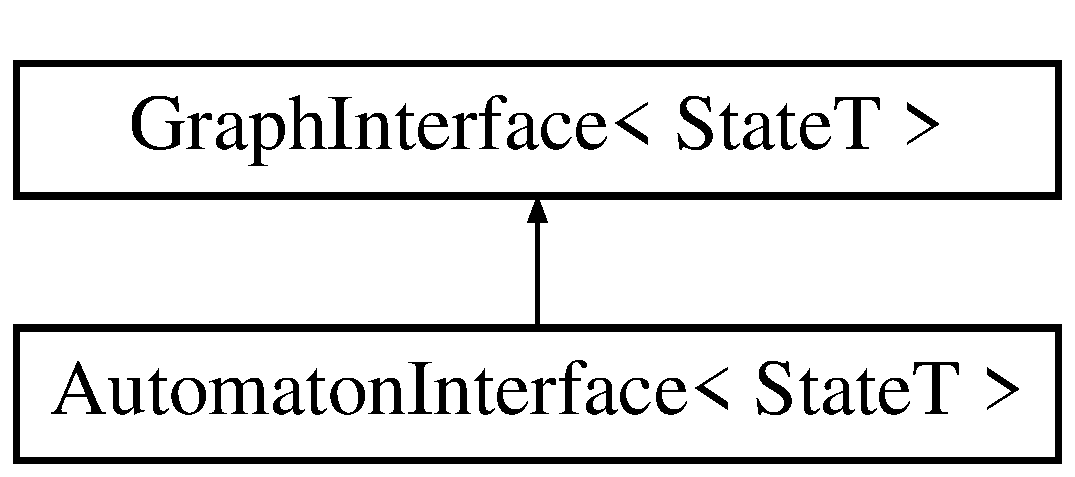
\includegraphics[height=2.000000cm]{classGraphInterface}
\end{center}
\end{figure}
\subsection*{\-Public \-Member \-Functions}
\begin{DoxyCompactItemize}
\item 
std\-::size\-\_\-t \hyperlink{classGraphInterface_a826adfb63a3a03795b0b15c4cff2a414}{get\-State\-Count} () const 
\item 
std\-::size\-\_\-t \hyperlink{classGraphInterface_af91873935ea90cce19f9db607f905071}{get\-Transition\-Count} (const \-State\-I\-D \-I\-D) const 
\item 
\-State\-I\-D \hyperlink{classGraphInterface_ac0479fb67be175a92af216a6901d721d}{get\-Target\-I\-D} (const \-State\-I\-D \-I\-D, const std\-::size\-\_\-t transition\-\_\-number) const 
\item 
const std\-::string \& \hyperlink{classGraphInterface_af05eafbb06b45872478168868d6747d9}{get\-String} (const \-State\-I\-D \-I\-D) const 
\end{DoxyCompactItemize}
\subsection*{\-Protected \-Attributes}
\begin{DoxyCompactItemize}
\item 
\hypertarget{classGraphInterface_af177873052deecf8de9f3eb3daa3b7e3}{std\-::vector$<$ \-State\-T $>$ \hyperlink{classGraphInterface_af177873052deecf8de9f3eb3daa3b7e3}{states}}\label{classGraphInterface_af177873052deecf8de9f3eb3daa3b7e3}

\begin{DoxyCompactList}\small\item\em \-Vector holding states of the graph. \end{DoxyCompactList}\end{DoxyCompactItemize}
\subsubsection*{template$<$typename \-State\-T$>$ class Graph\-Interface$<$ State\-T $>$}



\subsection{\-Member \-Function \-Documentation}
\hypertarget{classGraphInterface_a826adfb63a3a03795b0b15c4cff2a414}{\index{\-Graph\-Interface@{\-Graph\-Interface}!get\-State\-Count@{get\-State\-Count}}
\index{get\-State\-Count@{get\-State\-Count}!GraphInterface@{\-Graph\-Interface}}
\subsubsection[{get\-State\-Count}]{\setlength{\rightskip}{0pt plus 5cm}template$<$typename \-State\-T$>$ std\-::size\-\_\-t {\bf \-Graph\-Interface}$<$ \-State\-T $>$\-::{\bf get\-State\-Count} (
\begin{DoxyParamCaption}
{}
\end{DoxyParamCaption}
) const\hspace{0.3cm}{\ttfamily  \mbox{[}inline\mbox{]}}}}\label{classGraphInterface_a826adfb63a3a03795b0b15c4cff2a414}
\-Obtains number of states of the graph.

\begin{DoxyReturn}{\-Returns}
integer with size of the graph 
\end{DoxyReturn}
\hypertarget{classGraphInterface_af05eafbb06b45872478168868d6747d9}{\index{\-Graph\-Interface@{\-Graph\-Interface}!get\-String@{get\-String}}
\index{get\-String@{get\-String}!GraphInterface@{\-Graph\-Interface}}
\subsubsection[{get\-String}]{\setlength{\rightskip}{0pt plus 5cm}template$<$typename \-State\-T$>$ const std\-::string\& {\bf \-Graph\-Interface}$<$ \-State\-T $>$\-::{\bf get\-String} (
\begin{DoxyParamCaption}
\item[{const \-State\-I\-D}]{\-I\-D}
\end{DoxyParamCaption}
) const\hspace{0.3cm}{\ttfamily  \mbox{[}inline\mbox{]}}}}\label{classGraphInterface_af05eafbb06b45872478168868d6747d9}
\-Returns given state as a string.


\begin{DoxyParams}{\-Parameters}
{\em \-I\-D} & \-I\-D of the state to turn into the string\\
\hline
\end{DoxyParams}
\begin{DoxyReturn}{\-Returns}
given state as a string 
\end{DoxyReturn}
\hypertarget{classGraphInterface_ac0479fb67be175a92af216a6901d721d}{\index{\-Graph\-Interface@{\-Graph\-Interface}!get\-Target\-I\-D@{get\-Target\-I\-D}}
\index{get\-Target\-I\-D@{get\-Target\-I\-D}!GraphInterface@{\-Graph\-Interface}}
\subsubsection[{get\-Target\-I\-D}]{\setlength{\rightskip}{0pt plus 5cm}template$<$typename \-State\-T$>$ \-State\-I\-D {\bf \-Graph\-Interface}$<$ \-State\-T $>$\-::{\bf get\-Target\-I\-D} (
\begin{DoxyParamCaption}
\item[{const \-State\-I\-D}]{\-I\-D, }
\item[{const std\-::size\-\_\-t}]{transition\-\_\-number}
\end{DoxyParamCaption}
) const\hspace{0.3cm}{\ttfamily  \mbox{[}inline\mbox{]}}}}\label{classGraphInterface_ac0479fb67be175a92af216a6901d721d}
\-Obtains \-I\-D of the target of given transition for given state.


\begin{DoxyParams}{\-Parameters}
{\em \-I\-D} & \-I\-D of the state to get the neighbour from \\
\hline
{\em trans\-\_\-number} & index in the vector of transitions\\
\hline
\end{DoxyParams}
\begin{DoxyReturn}{\-Returns}
\-I\-D of the requested target 
\end{DoxyReturn}
\hypertarget{classGraphInterface_af91873935ea90cce19f9db607f905071}{\index{\-Graph\-Interface@{\-Graph\-Interface}!get\-Transition\-Count@{get\-Transition\-Count}}
\index{get\-Transition\-Count@{get\-Transition\-Count}!GraphInterface@{\-Graph\-Interface}}
\subsubsection[{get\-Transition\-Count}]{\setlength{\rightskip}{0pt plus 5cm}template$<$typename \-State\-T$>$ std\-::size\-\_\-t {\bf \-Graph\-Interface}$<$ \-State\-T $>$\-::{\bf get\-Transition\-Count} (
\begin{DoxyParamCaption}
\item[{const \-State\-I\-D}]{\-I\-D}
\end{DoxyParamCaption}
) const\hspace{0.3cm}{\ttfamily  \mbox{[}inline\mbox{]}}}}\label{classGraphInterface_af91873935ea90cce19f9db607f905071}
\-Obtains number of outcoming transitions for given state.


\begin{DoxyParams}{\-Parameters}
{\em \-I\-D} & \-I\-D of the state to get the number from\\
\hline
\end{DoxyParams}
\begin{DoxyReturn}{\-Returns}
integer with number of outcoming transitions 
\end{DoxyReturn}


\-The documentation for this class was generated from the following file\-:\begin{DoxyCompactItemize}
\item 
construction/graph\-\_\-interface.\-hpp\end{DoxyCompactItemize}

\hypertarget{classLabelingBuilder}{\section{\-Labeling\-Builder \-Class \-Reference}
\label{classLabelingBuilder}\index{\-Labeling\-Builder@{\-Labeling\-Builder}}
}


\-Creates a labeled graph representation of gene regulatory network and stores it within a \hyperlink{classLabelingHolder}{\-Labeling\-Holder} object.  




{\ttfamily \#include $<$labeling\-\_\-builder.\-hpp$>$}

\subsection*{\-Public \-Member \-Functions}
\begin{DoxyCompactItemize}
\item 
\hyperlink{classLabelingBuilder_ac8ddbe70fac49c0a2d0da8ee44881584}{\-Labeling\-Builder} (const \hyperlink{classModel}{\-Model} \&\-\_\-model, const \hyperlink{classParametrizationsHolder}{\-Parametrizations\-Holder} \&\-\_\-parametrizations, \hyperlink{classLabelingHolder}{\-Labeling\-Holder} \&\-\_\-labeling\-\_\-holder)
\item 
void \hyperlink{classLabelingBuilder_a7d43d3cd8ccbc4b0df48b48a4d76020f}{build\-Labeling} ()
\end{DoxyCompactItemize}


\subsection{\-Constructor \& \-Destructor \-Documentation}
\hypertarget{classLabelingBuilder_ac8ddbe70fac49c0a2d0da8ee44881584}{\index{\-Labeling\-Builder@{\-Labeling\-Builder}!\-Labeling\-Builder@{\-Labeling\-Builder}}
\index{\-Labeling\-Builder@{\-Labeling\-Builder}!LabelingBuilder@{\-Labeling\-Builder}}
\subsubsection[{\-Labeling\-Builder}]{\setlength{\rightskip}{0pt plus 5cm}\-Labeling\-Builder\-::\-Labeling\-Builder (
\begin{DoxyParamCaption}
\item[{const {\bf \-Model} \&}]{\-\_\-model, }
\item[{const {\bf \-Parametrizations\-Holder} \&}]{\-\_\-parametrizations, }
\item[{{\bf \-Labeling\-Holder} \&}]{\-\_\-labeling\-\_\-holder}
\end{DoxyParamCaption}
)\hspace{0.3cm}{\ttfamily  \mbox{[}inline\mbox{]}}}}\label{classLabelingBuilder_ac8ddbe70fac49c0a2d0da8ee44881584}
\-Constructor just attaches the references to data holders 

\subsection{\-Member \-Function \-Documentation}
\hypertarget{classLabelingBuilder_a7d43d3cd8ccbc4b0df48b48a4d76020f}{\index{\-Labeling\-Builder@{\-Labeling\-Builder}!build\-Labeling@{build\-Labeling}}
\index{build\-Labeling@{build\-Labeling}!LabelingBuilder@{\-Labeling\-Builder}}
\subsubsection[{build\-Labeling}]{\setlength{\rightskip}{0pt plus 5cm}void {\bf \-Labeling\-Builder\-::build\-Labeling} (
\begin{DoxyParamCaption}
{}
\end{DoxyParamCaption}
)\hspace{0.3cm}{\ttfamily  \mbox{[}inline\mbox{]}}}}\label{classLabelingBuilder_a7d43d3cd8ccbc4b0df48b48a4d76020f}
\-For each specie recreate all its regulatory functions (all possible labels) 

\-The documentation for this class was generated from the following file\-:\begin{DoxyCompactItemize}
\item 
construction/labeling\-\_\-builder.\-hpp\end{DoxyCompactItemize}

\hypertarget{classLabelingHolder}{\section{\-Labeling\-Holder \-Class \-Reference}
\label{classLabelingHolder}\index{\-Labeling\-Holder@{\-Labeling\-Holder}}
}


\-Storage for the regulatory graph with kinetic parameters encoded in form of regulatory functions.  




{\ttfamily \#include $<$labeling\-\_\-holder.\-hpp$>$}

\subsection*{\-Classes}
\begin{DoxyCompactItemize}
\item 
struct {\bfseries \-Regulatory\-Function}
\begin{DoxyCompactList}\small\item\em \-Storing a regulatory function in explicit form. \end{DoxyCompactList}\item 
struct {\bfseries \-Specie}
\begin{DoxyCompactList}\small\item\em \-Storing a sigle specie with its regulations. \end{DoxyCompactList}\end{DoxyCompactItemize}
\subsection*{\-Public \-Member \-Functions}
\begin{DoxyCompactItemize}
\item 
\hypertarget{classLabelingHolder_a6650bbd2ca3642b7733d7d7c986a8582}{\hyperlink{classLabelingHolder_a6650bbd2ca3642b7733d7d7c986a8582}{\-Labeling\-Holder} ()}\label{classLabelingHolder_a6650bbd2ca3642b7733d7d7c986a8582}

\begin{DoxyCompactList}\small\item\em \-Default empty constructor. \end{DoxyCompactList}\item 
std\-::size\-\_\-t \hyperlink{classLabelingHolder_a16cc2c15870a02f05e6a338ee451edd2}{get\-Parameters\-Count} () const 
\item 
std\-::size\-\_\-t \hyperlink{classLabelingHolder_a10c982727e0b71b5ac349cbc947d6dfe}{get\-Species\-Count} () const 
\item 
const std\-::string \& \hyperlink{classLabelingHolder_ac32b9124f9ff54b2e248bc07a249c78f}{get\-Specie\-Name} (const std\-::size\-\_\-t \-I\-D) const 
\item 
const std\-::vector$<$ std\-::size\-\_\-t $>$ \& \hyperlink{classLabelingHolder_a2bdbf8d0944eeb84d3cd2813f2795cf2}{get\-Specie\-Values} (const std\-::size\-\_\-t \-I\-D) const 
\item 
const std\-::vector$<$ std\-::size\-\_\-t $>$ \& \hyperlink{classLabelingHolder_aff60562d4517d58bd6be72afe0a04bed}{get\-Source\-Species} (const std\-::size\-\_\-t \-I\-D) const 
\item 
std\-::size\-\_\-t \hyperlink{classLabelingHolder_a7dcac5bcc2ffe7af9c81dd3d3856f6b6}{get\-Regulations\-Count} (const std\-::size\-\_\-t \-I\-D) const 
\item 
std\-::size\-\_\-t \hyperlink{classLabelingHolder_abd0a87a2878d1424c1e0d58a016e43d5}{get\-Step\-Size} (const std\-::size\-\_\-t \-I\-D, const std\-::size\-\_\-t regulation) const 
\item 
const std\-::vector$<$ std\-::size\-\_\-t $>$ \& \hyperlink{classLabelingHolder_a0ebe90fed8975996e71614919454b05e}{get\-Possible\-Values} (const std\-::size\-\_\-t \-I\-D, const std\-::size\-\_\-t regulation) const 
\item 
const std\-::vector$<$ std\-::vector\*
$<$ std\-::size\-\_\-t $>$ $>$ \& \hyperlink{classLabelingHolder_acc8f967132416e10fd6d4e5721093d87}{get\-Source\-Values} (const std\-::size\-\_\-t \-I\-D, const std\-::size\-\_\-t regulation) const 
\end{DoxyCompactItemize}
\subsection*{\-Friends}
\begin{DoxyCompactItemize}
\item 
\hypertarget{classLabelingHolder_af2136cc7df4f046e74b74f51de6901ac}{class {\bfseries \-Labeling\-Builder}}\label{classLabelingHolder_af2136cc7df4f046e74b74f51de6901ac}

\end{DoxyCompactItemize}


\subsection{\-Detailed \-Description}
\hyperlink{classLabelingHolder}{\-Labeling\-Holder} contains basic representation of the \-Gene \-Regulatory network in the form of the labeled graph. \-Each specie is stored together with its regulations. \-Each regulation has its step\-\_\-size value (shared by multiple regulations). \-This value represents division of parametrization space and is used for encoding and decoding it into paramset. \hyperlink{classLabelingHolder}{\-Labeling\-Holder} data can be set only form the \hyperlink{classLabelingBuilder}{\-Labeling\-Builder} object. 

\subsection{\-Member \-Function \-Documentation}
\hypertarget{classLabelingHolder_a16cc2c15870a02f05e6a338ee451edd2}{\index{\-Labeling\-Holder@{\-Labeling\-Holder}!get\-Parameters\-Count@{get\-Parameters\-Count}}
\index{get\-Parameters\-Count@{get\-Parameters\-Count}!LabelingHolder@{\-Labeling\-Holder}}
\subsubsection[{get\-Parameters\-Count}]{\setlength{\rightskip}{0pt plus 5cm}std\-::size\-\_\-t {\bf \-Labeling\-Holder\-::get\-Parameters\-Count} (
\begin{DoxyParamCaption}
{}
\end{DoxyParamCaption}
) const\hspace{0.3cm}{\ttfamily  \mbox{[}inline\mbox{]}}}}\label{classLabelingHolder_a16cc2c15870a02f05e6a338ee451edd2}
\begin{DoxyReturn}{\-Returns}
size of the parameter space 
\end{DoxyReturn}
\hypertarget{classLabelingHolder_a0ebe90fed8975996e71614919454b05e}{\index{\-Labeling\-Holder@{\-Labeling\-Holder}!get\-Possible\-Values@{get\-Possible\-Values}}
\index{get\-Possible\-Values@{get\-Possible\-Values}!LabelingHolder@{\-Labeling\-Holder}}
\subsubsection[{get\-Possible\-Values}]{\setlength{\rightskip}{0pt plus 5cm}const std\-::vector$<$std\-::size\-\_\-t$>$\& {\bf \-Labeling\-Holder\-::get\-Possible\-Values} (
\begin{DoxyParamCaption}
\item[{const std\-::size\-\_\-t}]{\-I\-D, }
\item[{const std\-::size\-\_\-t}]{regulation}
\end{DoxyParamCaption}
) const\hspace{0.3cm}{\ttfamily  \mbox{[}inline\mbox{]}}}}\label{classLabelingHolder_a0ebe90fed8975996e71614919454b05e}
\begin{DoxyReturn}{\-Returns}
values this function can possibly regulate to 
\end{DoxyReturn}
\hypertarget{classLabelingHolder_a7dcac5bcc2ffe7af9c81dd3d3856f6b6}{\index{\-Labeling\-Holder@{\-Labeling\-Holder}!get\-Regulations\-Count@{get\-Regulations\-Count}}
\index{get\-Regulations\-Count@{get\-Regulations\-Count}!LabelingHolder@{\-Labeling\-Holder}}
\subsubsection[{get\-Regulations\-Count}]{\setlength{\rightskip}{0pt plus 5cm}std\-::size\-\_\-t {\bf \-Labeling\-Holder\-::get\-Regulations\-Count} (
\begin{DoxyParamCaption}
\item[{const std\-::size\-\_\-t}]{\-I\-D}
\end{DoxyParamCaption}
) const\hspace{0.3cm}{\ttfamily  \mbox{[}inline\mbox{]}}}}\label{classLabelingHolder_a7dcac5bcc2ffe7af9c81dd3d3856f6b6}
\begin{DoxyReturn}{\-Returns}
number of regulations for this specie (two to power of number of source species) 
\end{DoxyReturn}
\hypertarget{classLabelingHolder_aff60562d4517d58bd6be72afe0a04bed}{\index{\-Labeling\-Holder@{\-Labeling\-Holder}!get\-Source\-Species@{get\-Source\-Species}}
\index{get\-Source\-Species@{get\-Source\-Species}!LabelingHolder@{\-Labeling\-Holder}}
\subsubsection[{get\-Source\-Species}]{\setlength{\rightskip}{0pt plus 5cm}const std\-::vector$<$std\-::size\-\_\-t$>$\& {\bf \-Labeling\-Holder\-::get\-Source\-Species} (
\begin{DoxyParamCaption}
\item[{const std\-::size\-\_\-t}]{\-I\-D}
\end{DoxyParamCaption}
) const\hspace{0.3cm}{\ttfamily  \mbox{[}inline\mbox{]}}}}\label{classLabelingHolder_aff60562d4517d58bd6be72afe0a04bed}
\begin{DoxyReturn}{\-Returns}
\-I\-Ds of all the species that regulate this specie 
\end{DoxyReturn}
\hypertarget{classLabelingHolder_acc8f967132416e10fd6d4e5721093d87}{\index{\-Labeling\-Holder@{\-Labeling\-Holder}!get\-Source\-Values@{get\-Source\-Values}}
\index{get\-Source\-Values@{get\-Source\-Values}!LabelingHolder@{\-Labeling\-Holder}}
\subsubsection[{get\-Source\-Values}]{\setlength{\rightskip}{0pt plus 5cm}const std\-::vector$<$std\-::vector$<$std\-::size\-\_\-t$>$ $>$\& {\bf \-Labeling\-Holder\-::get\-Source\-Values} (
\begin{DoxyParamCaption}
\item[{const std\-::size\-\_\-t}]{\-I\-D, }
\item[{const std\-::size\-\_\-t}]{regulation}
\end{DoxyParamCaption}
) const\hspace{0.3cm}{\ttfamily  \mbox{[}inline\mbox{]}}}}\label{classLabelingHolder_acc8f967132416e10fd6d4e5721093d87}
\begin{DoxyReturn}{\-Returns}
for each source specie all the values that if it is within them, it allows this function 
\end{DoxyReturn}
\hypertarget{classLabelingHolder_ac32b9124f9ff54b2e248bc07a249c78f}{\index{\-Labeling\-Holder@{\-Labeling\-Holder}!get\-Specie\-Name@{get\-Specie\-Name}}
\index{get\-Specie\-Name@{get\-Specie\-Name}!LabelingHolder@{\-Labeling\-Holder}}
\subsubsection[{get\-Specie\-Name}]{\setlength{\rightskip}{0pt plus 5cm}const std\-::string\& {\bf \-Labeling\-Holder\-::get\-Specie\-Name} (
\begin{DoxyParamCaption}
\item[{const std\-::size\-\_\-t}]{\-I\-D}
\end{DoxyParamCaption}
) const\hspace{0.3cm}{\ttfamily  \mbox{[}inline\mbox{]}}}}\label{classLabelingHolder_ac32b9124f9ff54b2e248bc07a249c78f}
\begin{DoxyReturn}{\-Returns}
name of the specie with given \-I\-D 
\end{DoxyReturn}
\hypertarget{classLabelingHolder_a10c982727e0b71b5ac349cbc947d6dfe}{\index{\-Labeling\-Holder@{\-Labeling\-Holder}!get\-Species\-Count@{get\-Species\-Count}}
\index{get\-Species\-Count@{get\-Species\-Count}!LabelingHolder@{\-Labeling\-Holder}}
\subsubsection[{get\-Species\-Count}]{\setlength{\rightskip}{0pt plus 5cm}std\-::size\-\_\-t {\bf \-Labeling\-Holder\-::get\-Species\-Count} (
\begin{DoxyParamCaption}
{}
\end{DoxyParamCaption}
) const\hspace{0.3cm}{\ttfamily  \mbox{[}inline\mbox{]}}}}\label{classLabelingHolder_a10c982727e0b71b5ac349cbc947d6dfe}
\begin{DoxyReturn}{\-Returns}
number of the species 
\end{DoxyReturn}
\hypertarget{classLabelingHolder_a2bdbf8d0944eeb84d3cd2813f2795cf2}{\index{\-Labeling\-Holder@{\-Labeling\-Holder}!get\-Specie\-Values@{get\-Specie\-Values}}
\index{get\-Specie\-Values@{get\-Specie\-Values}!LabelingHolder@{\-Labeling\-Holder}}
\subsubsection[{get\-Specie\-Values}]{\setlength{\rightskip}{0pt plus 5cm}const std\-::vector$<$std\-::size\-\_\-t$>$\& {\bf \-Labeling\-Holder\-::get\-Specie\-Values} (
\begin{DoxyParamCaption}
\item[{const std\-::size\-\_\-t}]{\-I\-D}
\end{DoxyParamCaption}
) const\hspace{0.3cm}{\ttfamily  \mbox{[}inline\mbox{]}}}}\label{classLabelingHolder_a2bdbf8d0944eeb84d3cd2813f2795cf2}
\begin{DoxyReturn}{\-Returns}
all the values the specie can occur in 
\end{DoxyReturn}
\hypertarget{classLabelingHolder_abd0a87a2878d1424c1e0d58a016e43d5}{\index{\-Labeling\-Holder@{\-Labeling\-Holder}!get\-Step\-Size@{get\-Step\-Size}}
\index{get\-Step\-Size@{get\-Step\-Size}!LabelingHolder@{\-Labeling\-Holder}}
\subsubsection[{get\-Step\-Size}]{\setlength{\rightskip}{0pt plus 5cm}std\-::size\-\_\-t {\bf \-Labeling\-Holder\-::get\-Step\-Size} (
\begin{DoxyParamCaption}
\item[{const std\-::size\-\_\-t}]{\-I\-D, }
\item[{const std\-::size\-\_\-t}]{regulation}
\end{DoxyParamCaption}
) const\hspace{0.3cm}{\ttfamily  \mbox{[}inline\mbox{]}}}}\label{classLabelingHolder_abd0a87a2878d1424c1e0d58a016e43d5}
\begin{DoxyReturn}{\-Returns}
step\-\_\-size (how many neigbour parameters share the same value for this regulation) 
\end{DoxyReturn}


\-The documentation for this class was generated from the following file\-:\begin{DoxyCompactItemize}
\item 
construction/labeling\-\_\-holder.\-hpp\end{DoxyCompactItemize}

\hypertarget{classModel}{\section{\-Model \-Class \-Reference}
\label{classModel}\index{\-Model@{\-Model}}
}


\-Storage for data parsed from the model.  




{\ttfamily \#include $<$model.\-hpp$>$}

\subsection*{\-Classes}
\begin{DoxyCompactItemize}
\item 
struct {\bfseries \-Additional\-Information}
\begin{DoxyCompactList}\small\item\em \-Structure that stores additional information about the model. \end{DoxyCompactList}\item 
struct {\bfseries \-Buchi\-Automaton\-State}
\begin{DoxyCompactList}\small\item\em \-Structure that holds data about a single state. \end{DoxyCompactList}\item 
struct {\bfseries \-Model\-Specie}
\begin{DoxyCompactList}\small\item\em \-Structure that holds data about a single specie. \-Most of the data is equal to that in the model file. \end{DoxyCompactList}\item 
struct \hyperlink{structModel_1_1Regulation}{\-Regulation}
\begin{DoxyCompactList}\small\item\em \-Structure that stores regulation of a specie by another one. \end{DoxyCompactList}\end{DoxyCompactItemize}
\subsection*{\-Public \-Types}
\begin{DoxyCompactItemize}
\item 
\hypertarget{classModel_a68b6cea215bd8221cc6f8de2a187b4b4}{typedef std\-::pair$<$ std\-::vector\*
$<$ bool $>$, int $>$ \hyperlink{classModel_a68b6cea215bd8221cc6f8de2a187b4b4}{\-Parameter}}\label{classModel_a68b6cea215bd8221cc6f8de2a187b4b4}

\begin{DoxyCompactList}\small\item\em \-Kinetic parameter of the specie (bitmask of active incoming regulations, target value) \end{DoxyCompactList}\item 
\hypertarget{classModel_a20d1a8ad1917da40f12e7ceb1f87d707}{typedef std\-::pair$<$ \-State\-I\-D, \*
std\-::string $>$ \hyperlink{classModel_a20d1a8ad1917da40f12e7ceb1f87d707}{\-Egde}}\label{classModel_a20d1a8ad1917da40f12e7ceb1f87d707}

\begin{DoxyCompactList}\small\item\em \-Edge in \-Buchi \-Automaton (\-Target \-I\-D, edge label) \end{DoxyCompactList}\end{DoxyCompactItemize}
\subsection*{\-Public \-Member \-Functions}
\begin{DoxyCompactItemize}
\item 
\hypertarget{classModel_ae3b375de5f6df4faf74a95d64748e048}{\hyperlink{classModel_ae3b375de5f6df4faf74a95d64748e048}{\-Model} ()}\label{classModel_ae3b375de5f6df4faf74a95d64748e048}

\begin{DoxyCompactList}\small\item\em \-Default empty constructor. \end{DoxyCompactList}\item 
std\-::size\-\_\-t \hyperlink{classModel_a31711d4597a1bcf090360bd6872cb048}{get\-Species\-Count} () const 
\item 
std\-::size\-\_\-t \hyperlink{classModel_aec5d5dd02fb170cd82ade21efda8ce39}{get\-States\-Count} () const 
\item 
\-Specie\-I\-D \hyperlink{classModel_a9459ce72805c7027e2d46263eca05424}{find\-I\-D} (const std\-::string \&name) const 
\item 
\-Specie\-I\-D \hyperlink{classModel_aa6acfd6cc4b416cdfdc402c8d0cffc44}{find\-Number} (const std\-::string \&name) const 
\item 
const std\-::string \& \hyperlink{classModel_a80f0c690cc256c060b235e3a8ba819a1}{get\-Name} (const std\-::size\-\_\-t \-I\-D) const 
\item 
std\-::size\-\_\-t \hyperlink{classModel_ab2215aa132f2c45e4c269d80c0e7bc5b}{get\-Min} (const std\-::size\-\_\-t \-I\-D) const 
\item 
std\-::size\-\_\-t \hyperlink{classModel_ae8b6f6313995b3bef5fc193b2aa4e48e}{get\-Max} (const std\-::size\-\_\-t \-I\-D) const 
\item 
std\-::size\-\_\-t \hyperlink{classModel_a77c551052d785251ab87291c084cc722}{get\-Basal} (const std\-::size\-\_\-t \-I\-D) const 
\item 
const std\-::vector$<$ \hyperlink{structModel_1_1Regulation}{\-Regulation} $>$ \& \hyperlink{classModel_af9cab24dce8973a2e9e510eae848cbd9}{get\-Regulations} (const std\-::size\-\_\-t \-I\-D) const 
\item 
const std\-::vector$<$ \hyperlink{classModel_a68b6cea215bd8221cc6f8de2a187b4b4}{\-Parameter} $>$ \& \hyperlink{classModel_a044064e89c7b62fd7d11a6fb26ce625d}{get\-Parameters} (const std\-::size\-\_\-t \-I\-D) const 
\item 
bool \hyperlink{classModel_ab14643d4a2af377f639d02b4c45ad486}{is\-Final} (const std\-::size\-\_\-t \-I\-D) const 
\item 
const std\-::vector$<$ \hyperlink{classModel_a20d1a8ad1917da40f12e7ceb1f87d707}{\-Egde} $>$ \& \hyperlink{classModel_abb52df1a8ca9abfddf430f43d2b674d7}{get\-Edges} (const std\-::size\-\_\-t \-I\-D) const 
\end{DoxyCompactItemize}
\subsection*{\-Friends}
\begin{DoxyCompactItemize}
\item 
\hypertarget{classModel_ac2bf95f4344eae6a1cfaa76928e21be0}{class {\bfseries \-Automaton\-Parser}}\label{classModel_ac2bf95f4344eae6a1cfaa76928e21be0}

\item 
\hypertarget{classModel_a2759f637c8f028a9ed4256db41bf34ac}{class {\bfseries \-Model\-Parser}}\label{classModel_a2759f637c8f028a9ed4256db41bf34ac}

\item 
\hypertarget{classModel_abc4942b2ed90a2f15b2421be44bc0d23}{class {\bfseries \-Network\-Parser}}\label{classModel_abc4942b2ed90a2f15b2421be44bc0d23}

\item 
\hypertarget{classModel_ac6ddcb9297cfa32e6c2c295dc70f371a}{class {\bfseries \-Time\-Series\-Parser}}\label{classModel_ac6ddcb9297cfa32e6c2c295dc70f371a}

\end{DoxyCompactItemize}


\subsection{\-Detailed \-Description}
\hyperlink{classModel}{\-Model} stores model data in the raw form, almost the same as in the model file itself. \hyperlink{classModel}{\-Model} data can be set only form the \hyperlink{classModelParser}{\-Model\-Parser} object. \-Rest of the code can access the data only via constant getters -\/ once the data are parse, model remains constant. 

\subsection{\-Member \-Function \-Documentation}
\hypertarget{classModel_a9459ce72805c7027e2d46263eca05424}{\index{\-Model@{\-Model}!find\-I\-D@{find\-I\-D}}
\index{find\-I\-D@{find\-I\-D}!Model@{\-Model}}
\subsubsection[{find\-I\-D}]{\setlength{\rightskip}{0pt plus 5cm}\-Specie\-I\-D {\bf \-Model\-::find\-I\-D} (
\begin{DoxyParamCaption}
\item[{const std\-::string \&}]{name}
\end{DoxyParamCaption}
) const\hspace{0.3cm}{\ttfamily  \mbox{[}inline\mbox{]}}}}\label{classModel_a9459ce72805c7027e2d46263eca05424}
\-Finds numerical \-I\-D of the specie based on its name or \-I\-D string.

\begin{DoxyReturn}{\-Returns}
\-I\-D of the specie with the specified name if there is such, otherwise $\sim$0 
\end{DoxyReturn}
\hypertarget{classModel_aa6acfd6cc4b416cdfdc402c8d0cffc44}{\index{\-Model@{\-Model}!find\-Number@{find\-Number}}
\index{find\-Number@{find\-Number}!Model@{\-Model}}
\subsubsection[{find\-Number}]{\setlength{\rightskip}{0pt plus 5cm}\-Specie\-I\-D {\bf \-Model\-::find\-Number} (
\begin{DoxyParamCaption}
\item[{const std\-::string \&}]{name}
\end{DoxyParamCaption}
) const\hspace{0.3cm}{\ttfamily  \mbox{[}inline\mbox{]}}}}\label{classModel_aa6acfd6cc4b416cdfdc402c8d0cffc44}
\-Finds ordinal number of the \-B\-A state based on its name or number string.

\begin{DoxyReturn}{\-Returns}
number of the state with the specified name if there is such, otherwise $\sim$0 
\end{DoxyReturn}
\hypertarget{classModel_a77c551052d785251ab87291c084cc722}{\index{\-Model@{\-Model}!get\-Basal@{get\-Basal}}
\index{get\-Basal@{get\-Basal}!Model@{\-Model}}
\subsubsection[{get\-Basal}]{\setlength{\rightskip}{0pt plus 5cm}std\-::size\-\_\-t {\bf \-Model\-::get\-Basal} (
\begin{DoxyParamCaption}
\item[{const std\-::size\-\_\-t}]{\-I\-D}
\end{DoxyParamCaption}
) const\hspace{0.3cm}{\ttfamily  \mbox{[}inline\mbox{]}}}}\label{classModel_a77c551052d785251ab87291c084cc722}
\begin{DoxyReturn}{\-Returns}
basal value of the specie 
\end{DoxyReturn}
\hypertarget{classModel_abb52df1a8ca9abfddf430f43d2b674d7}{\index{\-Model@{\-Model}!get\-Edges@{get\-Edges}}
\index{get\-Edges@{get\-Edges}!Model@{\-Model}}
\subsubsection[{get\-Edges}]{\setlength{\rightskip}{0pt plus 5cm}const std\-::vector$<${\bf \-Egde}$>$\& {\bf \-Model\-::get\-Edges} (
\begin{DoxyParamCaption}
\item[{const std\-::size\-\_\-t}]{\-I\-D}
\end{DoxyParamCaption}
) const\hspace{0.3cm}{\ttfamily  \mbox{[}inline\mbox{]}}}}\label{classModel_abb52df1a8ca9abfddf430f43d2b674d7}
\begin{DoxyReturn}{\-Returns}
edges of the state 
\end{DoxyReturn}
\hypertarget{classModel_ae8b6f6313995b3bef5fc193b2aa4e48e}{\index{\-Model@{\-Model}!get\-Max@{get\-Max}}
\index{get\-Max@{get\-Max}!Model@{\-Model}}
\subsubsection[{get\-Max}]{\setlength{\rightskip}{0pt plus 5cm}std\-::size\-\_\-t {\bf \-Model\-::get\-Max} (
\begin{DoxyParamCaption}
\item[{const std\-::size\-\_\-t}]{\-I\-D}
\end{DoxyParamCaption}
) const\hspace{0.3cm}{\ttfamily  \mbox{[}inline\mbox{]}}}}\label{classModel_ae8b6f6313995b3bef5fc193b2aa4e48e}
\begin{DoxyReturn}{\-Returns}
maximal value of the specie 
\end{DoxyReturn}
\hypertarget{classModel_ab2215aa132f2c45e4c269d80c0e7bc5b}{\index{\-Model@{\-Model}!get\-Min@{get\-Min}}
\index{get\-Min@{get\-Min}!Model@{\-Model}}
\subsubsection[{get\-Min}]{\setlength{\rightskip}{0pt plus 5cm}std\-::size\-\_\-t {\bf \-Model\-::get\-Min} (
\begin{DoxyParamCaption}
\item[{const std\-::size\-\_\-t}]{\-I\-D}
\end{DoxyParamCaption}
) const\hspace{0.3cm}{\ttfamily  \mbox{[}inline\mbox{]}}}}\label{classModel_ab2215aa132f2c45e4c269d80c0e7bc5b}
\begin{DoxyReturn}{\-Returns}
minimal value of the specie (always 0) 
\end{DoxyReturn}
\hypertarget{classModel_a80f0c690cc256c060b235e3a8ba819a1}{\index{\-Model@{\-Model}!get\-Name@{get\-Name}}
\index{get\-Name@{get\-Name}!Model@{\-Model}}
\subsubsection[{get\-Name}]{\setlength{\rightskip}{0pt plus 5cm}const std\-::string\& {\bf \-Model\-::get\-Name} (
\begin{DoxyParamCaption}
\item[{const std\-::size\-\_\-t}]{\-I\-D}
\end{DoxyParamCaption}
) const\hspace{0.3cm}{\ttfamily  \mbox{[}inline\mbox{]}}}}\label{classModel_a80f0c690cc256c060b235e3a8ba819a1}
\begin{DoxyReturn}{\-Returns}
name of the specie 
\end{DoxyReturn}
\hypertarget{classModel_a044064e89c7b62fd7d11a6fb26ce625d}{\index{\-Model@{\-Model}!get\-Parameters@{get\-Parameters}}
\index{get\-Parameters@{get\-Parameters}!Model@{\-Model}}
\subsubsection[{get\-Parameters}]{\setlength{\rightskip}{0pt plus 5cm}const std\-::vector$<${\bf \-Parameter}$>$\& {\bf \-Model\-::get\-Parameters} (
\begin{DoxyParamCaption}
\item[{const std\-::size\-\_\-t}]{\-I\-D}
\end{DoxyParamCaption}
) const\hspace{0.3cm}{\ttfamily  \mbox{[}inline\mbox{]}}}}\label{classModel_a044064e89c7b62fd7d11a6fb26ce625d}
\begin{DoxyReturn}{\-Returns}
kinetic parameters of the regulations of the specie 
\end{DoxyReturn}
\hypertarget{classModel_af9cab24dce8973a2e9e510eae848cbd9}{\index{\-Model@{\-Model}!get\-Regulations@{get\-Regulations}}
\index{get\-Regulations@{get\-Regulations}!Model@{\-Model}}
\subsubsection[{get\-Regulations}]{\setlength{\rightskip}{0pt plus 5cm}const std\-::vector$<${\bf \-Regulation}$>$\& {\bf \-Model\-::get\-Regulations} (
\begin{DoxyParamCaption}
\item[{const std\-::size\-\_\-t}]{\-I\-D}
\end{DoxyParamCaption}
) const\hspace{0.3cm}{\ttfamily  \mbox{[}inline\mbox{]}}}}\label{classModel_af9cab24dce8973a2e9e510eae848cbd9}
\begin{DoxyReturn}{\-Returns}
regulations of the specie 
\end{DoxyReturn}
\hypertarget{classModel_a31711d4597a1bcf090360bd6872cb048}{\index{\-Model@{\-Model}!get\-Species\-Count@{get\-Species\-Count}}
\index{get\-Species\-Count@{get\-Species\-Count}!Model@{\-Model}}
\subsubsection[{get\-Species\-Count}]{\setlength{\rightskip}{0pt plus 5cm}std\-::size\-\_\-t {\bf \-Model\-::get\-Species\-Count} (
\begin{DoxyParamCaption}
{}
\end{DoxyParamCaption}
) const\hspace{0.3cm}{\ttfamily  \mbox{[}inline\mbox{]}}}}\label{classModel_a31711d4597a1bcf090360bd6872cb048}
\begin{DoxyReturn}{\-Returns}
number of the species 
\end{DoxyReturn}
\hypertarget{classModel_aec5d5dd02fb170cd82ade21efda8ce39}{\index{\-Model@{\-Model}!get\-States\-Count@{get\-States\-Count}}
\index{get\-States\-Count@{get\-States\-Count}!Model@{\-Model}}
\subsubsection[{get\-States\-Count}]{\setlength{\rightskip}{0pt plus 5cm}std\-::size\-\_\-t {\bf \-Model\-::get\-States\-Count} (
\begin{DoxyParamCaption}
{}
\end{DoxyParamCaption}
) const\hspace{0.3cm}{\ttfamily  \mbox{[}inline\mbox{]}}}}\label{classModel_aec5d5dd02fb170cd82ade21efda8ce39}
\begin{DoxyReturn}{\-Returns}
number of the states 
\end{DoxyReturn}
\hypertarget{classModel_ab14643d4a2af377f639d02b4c45ad486}{\index{\-Model@{\-Model}!is\-Final@{is\-Final}}
\index{is\-Final@{is\-Final}!Model@{\-Model}}
\subsubsection[{is\-Final}]{\setlength{\rightskip}{0pt plus 5cm}bool {\bf \-Model\-::is\-Final} (
\begin{DoxyParamCaption}
\item[{const std\-::size\-\_\-t}]{\-I\-D}
\end{DoxyParamCaption}
) const\hspace{0.3cm}{\ttfamily  \mbox{[}inline\mbox{]}}}}\label{classModel_ab14643d4a2af377f639d02b4c45ad486}
\begin{DoxyReturn}{\-Returns}
true if the state is final 
\end{DoxyReturn}


\-The documentation for this class was generated from the following file\-:\begin{DoxyCompactItemize}
\item 
parsing/model.\-hpp\end{DoxyCompactItemize}

\hypertarget{classModelChecker}{\section{\-Model\-Checker \-Class \-Reference}
\label{classModelChecker}\index{\-Model\-Checker@{\-Model\-Checker}}
}


\-Main class of the computation -\/ responsible for the \-C\-M\-C procedure.  




{\ttfamily \#include $<$model\-\_\-checker.\-hpp$>$}

\subsection*{\-Public \-Member \-Functions}
\begin{DoxyCompactItemize}
\item 
\hyperlink{classModelChecker_af27cb475a7aa17cc378e6dbd0d55eb6b}{\-Model\-Checker} (const \hyperlink{classConstructionHolder}{\-Construction\-Holder} \&holder, \hyperlink{classColorStorage}{\-Color\-Storage} \&\-\_\-storage)
\item 
void \hyperlink{classModelChecker_a647ede3601153d3ce66a46c99673b3cd}{start\-Coloring} (const \-State\-I\-D \-I\-D, const \-Paramset parameters, const \-Range \&\-\_\-range)
\item 
void \hyperlink{classModelChecker_a532cf29476539edd24925204650ef1dc}{start\-Coloring} (const \-Paramset parameters, const std\-::set$<$ \-State\-I\-D $>$ \&\-\_\-updates, const \-Range \&\-\_\-range)
\end{DoxyCompactItemize}


\subsection{\-Detailed \-Description}
\hyperlink{classModelChecker}{\-Model\-Checker} class solves the parameter synthesis problem by iterative transfer of feasible parametrizations from initial states to final ones. \-Functions in model checker use many supporting variables and therefore are quite long, it would not make sense to split them, though. 

\subsection{\-Constructor \& \-Destructor \-Documentation}
\hypertarget{classModelChecker_af27cb475a7aa17cc378e6dbd0d55eb6b}{\index{\-Model\-Checker@{\-Model\-Checker}!\-Model\-Checker@{\-Model\-Checker}}
\index{\-Model\-Checker@{\-Model\-Checker}!ModelChecker@{\-Model\-Checker}}
\subsubsection[{\-Model\-Checker}]{\setlength{\rightskip}{0pt plus 5cm}\-Model\-Checker\-::\-Model\-Checker (
\begin{DoxyParamCaption}
\item[{const {\bf \-Construction\-Holder} \&}]{holder, }
\item[{{\bf \-Color\-Storage} \&}]{\-\_\-storage}
\end{DoxyParamCaption}
)\hspace{0.3cm}{\ttfamily  \mbox{[}inline\mbox{]}}}}\label{classModelChecker_af27cb475a7aa17cc378e6dbd0d55eb6b}
\-Constructor, passes the data and sets up auxiliary storage. 

\subsection{\-Member \-Function \-Documentation}
\hypertarget{classModelChecker_a647ede3601153d3ce66a46c99673b3cd}{\index{\-Model\-Checker@{\-Model\-Checker}!start\-Coloring@{start\-Coloring}}
\index{start\-Coloring@{start\-Coloring}!ModelChecker@{\-Model\-Checker}}
\subsubsection[{start\-Coloring}]{\setlength{\rightskip}{0pt plus 5cm}void {\bf \-Model\-Checker\-::start\-Coloring} (
\begin{DoxyParamCaption}
\item[{const \-State\-I\-D}]{\-I\-D, }
\item[{const \-Paramset}]{parameters, }
\item[{const \-Range \&}]{\-\_\-range}
\end{DoxyParamCaption}
)\hspace{0.3cm}{\ttfamily  \mbox{[}inline\mbox{]}}}}\label{classModelChecker_a647ede3601153d3ce66a46c99673b3cd}
\-Start a new coloring round for cycle detection from a single state.


\begin{DoxyParams}{\-Parameters}
{\em \-I\-D} & \-I\-D of the state to start cycle detection from \\
\hline
{\em parameters} & starting parameters for the cycle detection \\
\hline
{\em \-\_\-range} & range of parameters for this coloring round \\
\hline
\end{DoxyParams}
\hypertarget{classModelChecker_a532cf29476539edd24925204650ef1dc}{\index{\-Model\-Checker@{\-Model\-Checker}!start\-Coloring@{start\-Coloring}}
\index{start\-Coloring@{start\-Coloring}!ModelChecker@{\-Model\-Checker}}
\subsubsection[{start\-Coloring}]{\setlength{\rightskip}{0pt plus 5cm}void {\bf \-Model\-Checker\-::start\-Coloring} (
\begin{DoxyParamCaption}
\item[{const \-Paramset}]{parameters, }
\item[{const std\-::set$<$ \-State\-I\-D $>$ \&}]{\-\_\-updates, }
\item[{const \-Range \&}]{\-\_\-range}
\end{DoxyParamCaption}
)\hspace{0.3cm}{\ttfamily  \mbox{[}inline\mbox{]}}}}\label{classModelChecker_a532cf29476539edd24925204650ef1dc}
\-Start a new coloring round for cycle detection from a single state.


\begin{DoxyParams}{\-Parameters}
{\em parameters} & starting parameters to color the structure with \\
\hline
{\em \-\_\-updates} & states that are will be scheduled for an update in this round \\
\hline
{\em \-\_\-range} & range of parameters for this coloring round \\
\hline
\end{DoxyParams}


\-The documentation for this class was generated from the following file\-:\begin{DoxyCompactItemize}
\item 
synthesis/model\-\_\-checker.\-hpp\end{DoxyCompactItemize}

\hypertarget{classModelParser}{\section{\-Model\-Parser \-Class \-Reference}
\label{classModelParser}\index{\-Model\-Parser@{\-Model\-Parser}}
}


\-Starting point of the model parsing.  




{\ttfamily \#include $<$model\-\_\-parser.\-hpp$>$}

\subsection*{\-Public \-Member \-Functions}
\begin{DoxyCompactItemize}
\item 
\hypertarget{classModelParser_ac3c896f59f3bb10fa61d93b6c7300452}{\hyperlink{classModelParser_ac3c896f59f3bb10fa61d93b6c7300452}{\-Model\-Parser} (\hyperlink{classModel}{\-Model} \&\-\_\-model, std\-::ifstream $\ast$\-\_\-input\-\_\-stream)}\label{classModelParser_ac3c896f59f3bb10fa61d93b6c7300452}

\begin{DoxyCompactList}\small\item\em \-Simple constructor, passes references. \end{DoxyCompactList}\item 
void \hyperlink{classModelParser_ae2d3baf6ad332bc6c618a39b2d2fc27e}{parse\-Input} ()
\end{DoxyCompactItemize}


\subsection{\-Detailed \-Description}
\hyperlink{classModelParser}{\-Model\-Parser} is an entry point for parsing of a model file. \-Most of the parsing is done by dependent classes, \hyperlink{classModelParser}{\-Model\-Parser} only sets the parsing up for further usage. \-For the reference on how to create a model see the manual/\-R\-E\-A\-D\-M\-E. 

\subsection{\-Member \-Function \-Documentation}
\hypertarget{classModelParser_ae2d3baf6ad332bc6c618a39b2d2fc27e}{\index{\-Model\-Parser@{\-Model\-Parser}!parse\-Input@{parse\-Input}}
\index{parse\-Input@{parse\-Input}!ModelParser@{\-Model\-Parser}}
\subsubsection[{parse\-Input}]{\setlength{\rightskip}{0pt plus 5cm}void {\bf \-Model\-Parser\-::parse\-Input} (
\begin{DoxyParamCaption}
{}
\end{DoxyParamCaption}
)\hspace{0.3cm}{\ttfamily  \mbox{[}inline\mbox{]}}}}\label{classModelParser_ae2d3baf6ad332bc6c618a39b2d2fc27e}
\-Functions that causes the parser to read the input from the stream, parse it and store model information in the model object. 

\-The documentation for this class was generated from the following file\-:\begin{DoxyCompactItemize}
\item 
parsing/model\-\_\-parser.\-hpp\end{DoxyCompactItemize}

\hypertarget{classNetworkParser}{\section{\-Network\-Parser \-Class \-Reference}
\label{classNetworkParser}\index{\-Network\-Parser@{\-Network\-Parser}}
}


\-Class for parsing of the regulatory network.  




{\ttfamily \#include $<$network\-\_\-parser.\-hpp$>$}

\subsection*{\-Public \-Member \-Functions}
\begin{DoxyCompactItemize}
\item 
\hypertarget{classNetworkParser_ab48391bfccd5387f4a29ebbd22dd03a2}{\hyperlink{classNetworkParser_ab48391bfccd5387f4a29ebbd22dd03a2}{\-Network\-Parser} (\hyperlink{classModel}{\-Model} \&\-\_\-model)}\label{classNetworkParser_ab48391bfccd5387f4a29ebbd22dd03a2}

\begin{DoxyCompactList}\small\item\em \-Simple constructor, passes references. \end{DoxyCompactList}\item 
void \hyperlink{classNetworkParser_ac46f3ee893609c44f135551ee20009f6}{parse} (const rapidxml\-::xml\-\_\-node$<$$>$ $\ast$const model\-\_\-node)
\end{DoxyCompactItemize}


\subsection{\-Detailed \-Description}
\-This object is responsible for parsing and translation of data related to the \-G\-R\-N. \-Most of the possible semantics mistakes are under control and cause exceptions. 

\subsection{\-Member \-Function \-Documentation}
\hypertarget{classNetworkParser_ac46f3ee893609c44f135551ee20009f6}{\index{\-Network\-Parser@{\-Network\-Parser}!parse@{parse}}
\index{parse@{parse}!NetworkParser@{\-Network\-Parser}}
\subsubsection[{parse}]{\setlength{\rightskip}{0pt plus 5cm}void {\bf \-Network\-Parser\-::parse} (
\begin{DoxyParamCaption}
\item[{const rapidxml\-::xml\-\_\-node$<$$>$ $\ast$const}]{model\-\_\-node}
\end{DoxyParamCaption}
)\hspace{0.3cm}{\ttfamily  \mbox{[}inline\mbox{]}}}}\label{classNetworkParser_ac46f3ee893609c44f135551ee20009f6}
\-Main parsing function. \-It expects a pointer to inside of a \-M\-O\-D\-E\-L node. 

\-The documentation for this class was generated from the following file\-:\begin{DoxyCompactItemize}
\item 
parsing/network\-\_\-parser.\-hpp\end{DoxyCompactItemize}

\hypertarget{classOutputManager}{\section{\-Output\-Manager \-Class \-Reference}
\label{classOutputManager}\index{\-Output\-Manager@{\-Output\-Manager}}
}


\-Class that outputs formatted resulting data.  




{\ttfamily \#include $<$output\-\_\-manager.\-hpp$>$}

\subsection*{\-Public \-Member \-Functions}
\begin{DoxyCompactItemize}
\item 
\hyperlink{classOutputManager_a02dfccbf1f4e1f4f61e7e7e8a2a97978}{\-Output\-Manager} (const \hyperlink{classColorStorage}{\-Color\-Storage} \&\-\_\-storage, const \hyperlink{classColoringAnalyzer}{\-Coloring\-Analyzer} \&\-\_\-analyzer, const \hyperlink{classSplitManager}{\-Split\-Manager} \&\-\_\-split\-\_\-manager, \hyperlink{classWitnessSearcher}{\-Witness\-Searcher} \&\-\_\-searcher, \hyperlink{classRobustnessCompute}{\-Robustness\-Compute} \&\-\_\-robustness)
\item 
void \hyperlink{classOutputManager_ad2fc6aa32779d30f69c600e5810126de}{output\-Summary} (const std\-::size\-\_\-t total\-\_\-count)
\item 
void \hyperlink{classOutputManager_aa3a6094bc7631bf8596fa29ff3e8e9e3}{output\-Round\-Num} ()
\item 
const std\-::vector$<$ std\-::string $>$ \hyperlink{classOutputManager_a7deb5d1b9ddb74848f9ea2e67cf47463}{get\-Costs} (const std\-::vector$<$ std\-::size\-\_\-t $>$ cost\-\_\-vals) const 
\item 
void \hyperlink{classOutputManager_af5e0986744d368e7e3e850d8ec7767b3}{output\-Round} () const 
\end{DoxyCompactItemize}


\subsection{\-Constructor \& \-Destructor \-Documentation}
\hypertarget{classOutputManager_a02dfccbf1f4e1f4f61e7e7e8a2a97978}{\index{\-Output\-Manager@{\-Output\-Manager}!\-Output\-Manager@{\-Output\-Manager}}
\index{\-Output\-Manager@{\-Output\-Manager}!OutputManager@{\-Output\-Manager}}
\subsubsection[{\-Output\-Manager}]{\setlength{\rightskip}{0pt plus 5cm}\-Output\-Manager\-::\-Output\-Manager (
\begin{DoxyParamCaption}
\item[{const {\bf \-Color\-Storage} \&}]{\-\_\-storage, }
\item[{const {\bf \-Coloring\-Analyzer} \&}]{\-\_\-analyzer, }
\item[{const {\bf \-Split\-Manager} \&}]{\-\_\-split\-\_\-manager, }
\item[{{\bf \-Witness\-Searcher} \&}]{\-\_\-searcher, }
\item[{{\bf \-Robustness\-Compute} \&}]{\-\_\-robustness}
\end{DoxyParamCaption}
)\hspace{0.3cm}{\ttfamily  \mbox{[}inline\mbox{]}}}}\label{classOutputManager_a02dfccbf1f4e1f4f61e7e7e8a2a97978}
\-Simple constructor that only passes the references. 

\subsection{\-Member \-Function \-Documentation}
\hypertarget{classOutputManager_a7deb5d1b9ddb74848f9ea2e67cf47463}{\index{\-Output\-Manager@{\-Output\-Manager}!get\-Costs@{get\-Costs}}
\index{get\-Costs@{get\-Costs}!OutputManager@{\-Output\-Manager}}
\subsubsection[{get\-Costs}]{\setlength{\rightskip}{0pt plus 5cm}const std\-::vector$<$std\-::string$>$ {\bf \-Output\-Manager\-::get\-Costs} (
\begin{DoxyParamCaption}
\item[{const std\-::vector$<$ std\-::size\-\_\-t $>$}]{cost\-\_\-vals}
\end{DoxyParamCaption}
) const\hspace{0.3cm}{\ttfamily  \mbox{[}inline\mbox{]}}}}\label{classOutputManager_a7deb5d1b9ddb74848f9ea2e67cf47463}
\-Recreate vector of cost values into a vector of strings. \hypertarget{classOutputManager_af5e0986744d368e7e3e850d8ec7767b3}{\index{\-Output\-Manager@{\-Output\-Manager}!output\-Round@{output\-Round}}
\index{output\-Round@{output\-Round}!OutputManager@{\-Output\-Manager}}
\subsubsection[{output\-Round}]{\setlength{\rightskip}{0pt plus 5cm}void {\bf \-Output\-Manager\-::output\-Round} (
\begin{DoxyParamCaption}
{}
\end{DoxyParamCaption}
) const\hspace{0.3cm}{\ttfamily  \mbox{[}inline\mbox{]}}}}\label{classOutputManager_af5e0986744d368e7e3e850d8ec7767b3}
\-Display colors synthetized during current round. \hypertarget{classOutputManager_aa3a6094bc7631bf8596fa29ff3e8e9e3}{\index{\-Output\-Manager@{\-Output\-Manager}!output\-Round\-Num@{output\-Round\-Num}}
\index{output\-Round\-Num@{output\-Round\-Num}!OutputManager@{\-Output\-Manager}}
\subsubsection[{output\-Round\-Num}]{\setlength{\rightskip}{0pt plus 5cm}void {\bf \-Output\-Manager\-::output\-Round\-Num} (
\begin{DoxyParamCaption}
{}
\end{DoxyParamCaption}
)\hspace{0.3cm}{\ttfamily  \mbox{[}inline\mbox{]}}}}\label{classOutputManager_aa3a6094bc7631bf8596fa29ff3e8e9e3}
\-Outputs round number -\/ if there are no data within, then erase the line each round. \hypertarget{classOutputManager_ad2fc6aa32779d30f69c600e5810126de}{\index{\-Output\-Manager@{\-Output\-Manager}!output\-Summary@{output\-Summary}}
\index{output\-Summary@{output\-Summary}!OutputManager@{\-Output\-Manager}}
\subsubsection[{output\-Summary}]{\setlength{\rightskip}{0pt plus 5cm}void {\bf \-Output\-Manager\-::output\-Summary} (
\begin{DoxyParamCaption}
\item[{const std\-::size\-\_\-t}]{total\-\_\-count}
\end{DoxyParamCaption}
)\hspace{0.3cm}{\ttfamily  \mbox{[}inline\mbox{]}}}}\label{classOutputManager_ad2fc6aa32779d30f69c600e5810126de}
\-Output summary after the computation.


\begin{DoxyParams}{\-Parameters}
{\em total\-\_\-count} & number of all feasible colors \\
\hline
\end{DoxyParams}


\-The documentation for this class was generated from the following file\-:\begin{DoxyCompactItemize}
\item 
synthesis/output\-\_\-manager.\-hpp\end{DoxyCompactItemize}

\hypertarget{classOutputStreamer}{\section{\-Output\-Streamer \-Class \-Reference}
\label{classOutputStreamer}\index{\-Output\-Streamer@{\-Output\-Streamer}}
}


\-Class that contains methods for standard and special stream output.  




{\ttfamily \#include $<$output\-\_\-streamer.\-hpp$>$}

\subsection*{\-Public \-Types}
\begin{DoxyCompactItemize}
\item 
\hypertarget{classOutputStreamer_afde0341c035a66313bc0c473545564df}{typedef const unsigned int {\bfseries \-Trait}}\label{classOutputStreamer_afde0341c035a66313bc0c473545564df}

\end{DoxyCompactItemize}
\subsection*{\-Public \-Member \-Functions}
\begin{DoxyCompactItemize}
\item 
bool \hyperlink{classOutputStreamer_ac69a0b5740c6789c289f32a847497bcb}{test\-Trait} (const unsigned int tested, const unsigned int traits) const 
\item 
bool \hyperlink{classOutputStreamer_ad687fb52400ddead1bed0ea6d85fec71}{is\-Result\-In\-File} () const 
\item 
\hyperlink{classOutputStreamer_a300cf2cf0796ac9f32fa7706dfe6e3f7}{\-Output\-Streamer} ()
\item 
\hyperlink{classOutputStreamer_a2c5b231daa95e75e3d97412bf2825522}{$\sim$\-Output\-Streamer} ()
\item 
void \hyperlink{classOutputStreamer_a4f9075e1f4d0990da619fc82e648ed3a}{create\-Stream\-File} (\-Stream\-Type stream\-\_\-type, std\-::string filename)
\item 
void \hyperlink{classOutputStreamer_ab5ba0f1791ea756e826b4fa503420915}{flush} ()
\item 
{\footnotesize template$<$class output\-Type $>$ }\\const \hyperlink{classOutputStreamer}{\-Output\-Streamer} \& \hyperlink{classOutputStreamer_aca59f9ceafef1709da0c99b1d381be0a}{output} (\-Stream\-Type stream\-\_\-type, const output\-Type \&stream\-\_\-data, const unsigned int trait\-\_\-mask=0)
\item 
{\footnotesize template$<$class output\-Type $>$ }\\const \hyperlink{classOutputStreamer}{\-Output\-Streamer} \& \hyperlink{classOutputStreamer_a0b80cd3ff924882963e7f90bb2cdc1f2}{output} (const output\-Type \&stream\-\_\-data, const unsigned int trait\-\_\-mask=0) const 
\end{DoxyCompactItemize}
\subsection*{\-Static \-Public \-Attributes}
\begin{DoxyCompactItemize}
\item 
\hypertarget{classOutputStreamer_ac71ea1199278b1d27f8e02961e03324c}{static \-Trait \hyperlink{classOutputStreamer_ac71ea1199278b1d27f8e02961e03324c}{no\-\_\-newl} = 1}\label{classOutputStreamer_ac71ea1199278b1d27f8e02961e03324c}

\begin{DoxyCompactList}\small\item\em \-After last line no newline symbol will be output. \end{DoxyCompactList}\item 
\hypertarget{classOutputStreamer_a8c74dcf725523c8c1d310f3bcbebd58d}{static \-Trait \hyperlink{classOutputStreamer_a8c74dcf725523c8c1d310f3bcbebd58d}{important} = 2}\label{classOutputStreamer_a8c74dcf725523c8c1d310f3bcbebd58d}

\begin{DoxyCompactList}\small\item\em \-Add \char`\"{}-\/-\/ \char`\"{} before and \char`\"{} -\/-\/\char`\"{} after the ouptut. \end{DoxyCompactList}\item 
\hypertarget{classOutputStreamer_a96c1c4303f014a6eb83ab9635b783419}{static \-Trait \hyperlink{classOutputStreamer_a96c1c4303f014a6eb83ab9635b783419}{rewrite\-\_\-ln} = 4}\label{classOutputStreamer_a96c1c4303f014a6eb83ab9635b783419}

\begin{DoxyCompactList}\small\item\em \-Return the cursor and start from the beginning of the line. \end{DoxyCompactList}\item 
\hypertarget{classOutputStreamer_a993dfcb1247662943e1d45fac9e323d6}{static \-Trait \hyperlink{classOutputStreamer_a993dfcb1247662943e1d45fac9e323d6}{tab} = 8}\label{classOutputStreamer_a993dfcb1247662943e1d45fac9e323d6}

\begin{DoxyCompactList}\small\item\em \-Add \char`\"{}   \char`\"{} before the output. \end{DoxyCompactList}\end{DoxyCompactItemize}


\subsection{\-Constructor \& \-Destructor \-Documentation}
\hypertarget{classOutputStreamer_a300cf2cf0796ac9f32fa7706dfe6e3f7}{\index{\-Output\-Streamer@{\-Output\-Streamer}!\-Output\-Streamer@{\-Output\-Streamer}}
\index{\-Output\-Streamer@{\-Output\-Streamer}!OutputStreamer@{\-Output\-Streamer}}
\subsubsection[{\-Output\-Streamer}]{\setlength{\rightskip}{0pt plus 5cm}{\bf \-Output\-Streamer\-::\-Output\-Streamer} (
\begin{DoxyParamCaption}
{}
\end{DoxyParamCaption}
)\hspace{0.3cm}{\ttfamily  \mbox{[}inline\mbox{]}}}}\label{classOutputStreamer_a300cf2cf0796ac9f32fa7706dfe6e3f7}
\-Basic constructor -\/ should be used only for the single object shared throught the program. \hypertarget{classOutputStreamer_a2c5b231daa95e75e3d97412bf2825522}{\index{\-Output\-Streamer@{\-Output\-Streamer}!$\sim$\-Output\-Streamer@{$\sim$\-Output\-Streamer}}
\index{$\sim$\-Output\-Streamer@{$\sim$\-Output\-Streamer}!OutputStreamer@{\-Output\-Streamer}}
\subsubsection[{$\sim$\-Output\-Streamer}]{\setlength{\rightskip}{0pt plus 5cm}{\bf \-Output\-Streamer\-::$\sim$\-Output\-Streamer} (
\begin{DoxyParamCaption}
{}
\end{DoxyParamCaption}
)\hspace{0.3cm}{\ttfamily  \mbox{[}inline\mbox{]}}}}\label{classOutputStreamer_a2c5b231daa95e75e3d97412bf2825522}
\-If some of the streams has been assigned a file, delete that file object. 

\subsection{\-Member \-Function \-Documentation}
\hypertarget{classOutputStreamer_a4f9075e1f4d0990da619fc82e648ed3a}{\index{\-Output\-Streamer@{\-Output\-Streamer}!create\-Stream\-File@{create\-Stream\-File}}
\index{create\-Stream\-File@{create\-Stream\-File}!OutputStreamer@{\-Output\-Streamer}}
\subsubsection[{create\-Stream\-File}]{\setlength{\rightskip}{0pt plus 5cm}void {\bf \-Output\-Streamer\-::create\-Stream\-File} (
\begin{DoxyParamCaption}
\item[{\-Stream\-Type}]{stream\-\_\-type, }
\item[{std\-::string}]{filename}
\end{DoxyParamCaption}
)\hspace{0.3cm}{\ttfamily  \mbox{[}inline\mbox{]}}}}\label{classOutputStreamer_a4f9075e1f4d0990da619fc82e648ed3a}
\-Create a file to which given stream will be redirected.


\begin{DoxyParams}{\-Parameters}
{\em stream\-\_\-type} & enumeration type specifying the type of stream to output to \\
\hline
{\em data} & data to output -\/ should be any possible ostream data \\
\hline
\end{DoxyParams}
\hypertarget{classOutputStreamer_ab5ba0f1791ea756e826b4fa503420915}{\index{\-Output\-Streamer@{\-Output\-Streamer}!flush@{flush}}
\index{flush@{flush}!OutputStreamer@{\-Output\-Streamer}}
\subsubsection[{flush}]{\setlength{\rightskip}{0pt plus 5cm}void {\bf \-Output\-Streamer\-::flush} (
\begin{DoxyParamCaption}
{}
\end{DoxyParamCaption}
)\hspace{0.3cm}{\ttfamily  \mbox{[}inline\mbox{]}}}}\label{classOutputStreamer_ab5ba0f1791ea756e826b4fa503420915}
\-Flush all the streams that are in use. \hypertarget{classOutputStreamer_ad687fb52400ddead1bed0ea6d85fec71}{\index{\-Output\-Streamer@{\-Output\-Streamer}!is\-Result\-In\-File@{is\-Result\-In\-File}}
\index{is\-Result\-In\-File@{is\-Result\-In\-File}!OutputStreamer@{\-Output\-Streamer}}
\subsubsection[{is\-Result\-In\-File}]{\setlength{\rightskip}{0pt plus 5cm}bool {\bf \-Output\-Streamer\-::is\-Result\-In\-File} (
\begin{DoxyParamCaption}
{}
\end{DoxyParamCaption}
) const\hspace{0.3cm}{\ttfamily  \mbox{[}inline\mbox{]}}}}\label{classOutputStreamer_ad687fb52400ddead1bed0ea6d85fec71}
\begin{DoxyReturn}{\-Returns}
true if there is a file to output the results 
\end{DoxyReturn}
\hypertarget{classOutputStreamer_aca59f9ceafef1709da0c99b1d381be0a}{\index{\-Output\-Streamer@{\-Output\-Streamer}!output@{output}}
\index{output@{output}!OutputStreamer@{\-Output\-Streamer}}
\subsubsection[{output}]{\setlength{\rightskip}{0pt plus 5cm}template$<$class output\-Type $>$ const {\bf \-Output\-Streamer}\& {\bf \-Output\-Streamer\-::output} (
\begin{DoxyParamCaption}
\item[{\-Stream\-Type}]{stream\-\_\-type, }
\item[{const output\-Type \&}]{stream\-\_\-data, }
\item[{const unsigned int}]{trait\-\_\-mask = {\ttfamily 0}}
\end{DoxyParamCaption}
)\hspace{0.3cm}{\ttfamily  \mbox{[}inline\mbox{]}}}}\label{classOutputStreamer_aca59f9ceafef1709da0c99b1d381be0a}
\-Output on a specified stream.


\begin{DoxyParams}{\-Parameters}
{\em stream\-\_\-type} & enumeration type specifying the type of stream to output to \\
\hline
{\em data} & data to output -\/ should be any possible ostream data \\
\hline
{\em trait\-\_\-mask} & bitmask of traits for output \\
\hline
\end{DoxyParams}
\hypertarget{classOutputStreamer_a0b80cd3ff924882963e7f90bb2cdc1f2}{\index{\-Output\-Streamer@{\-Output\-Streamer}!output@{output}}
\index{output@{output}!OutputStreamer@{\-Output\-Streamer}}
\subsubsection[{output}]{\setlength{\rightskip}{0pt plus 5cm}template$<$class output\-Type $>$ const {\bf \-Output\-Streamer}\& {\bf \-Output\-Streamer\-::output} (
\begin{DoxyParamCaption}
\item[{const output\-Type \&}]{stream\-\_\-data, }
\item[{const unsigned int}]{trait\-\_\-mask = {\ttfamily 0}}
\end{DoxyParamCaption}
) const\hspace{0.3cm}{\ttfamily  \mbox{[}inline\mbox{]}}}}\label{classOutputStreamer_a0b80cd3ff924882963e7f90bb2cdc1f2}
\-Overloaded method that uses the same stream as the last ouput.


\begin{DoxyParams}{\-Parameters}
{\em data} & data to output -\/ should be any possible ostream data \\
\hline
{\em trait\-\_\-mask} & bitmask of traits for output \\
\hline
\end{DoxyParams}
\hypertarget{classOutputStreamer_ac69a0b5740c6789c289f32a847497bcb}{\index{\-Output\-Streamer@{\-Output\-Streamer}!test\-Trait@{test\-Trait}}
\index{test\-Trait@{test\-Trait}!OutputStreamer@{\-Output\-Streamer}}
\subsubsection[{test\-Trait}]{\setlength{\rightskip}{0pt plus 5cm}bool {\bf \-Output\-Streamer\-::test\-Trait} (
\begin{DoxyParamCaption}
\item[{const unsigned int}]{tested, }
\item[{const unsigned int}]{traits}
\end{DoxyParamCaption}
) const\hspace{0.3cm}{\ttfamily  \mbox{[}inline\mbox{]}}}}\label{classOutputStreamer_ac69a0b5740c6789c289f32a847497bcb}
\-Test if given trait is present.


\begin{DoxyParams}{\-Parameters}
{\em tested} & number of the tested trait \\
\hline
{\em traits} & traits given with the function\\
\hline
\end{DoxyParams}
\begin{DoxyReturn}{\-Returns}
bool if the trait is present 
\end{DoxyReturn}


\-The documentation for this class was generated from the following file\-:\begin{DoxyCompactItemize}
\item 
auxiliary/output\-\_\-streamer.\-hpp\end{DoxyCompactItemize}

\hypertarget{classParametrizationsBuilder}{\section{\-Parametrizations\-Builder \-Class \-Reference}
\label{classParametrizationsBuilder}\index{\-Parametrizations\-Builder@{\-Parametrizations\-Builder}}
}


\-Class that computes feasible parametrizations for each specie from edge constrains and stores them in a \-Parametrization\-Holder object.  




{\ttfamily \#include $<$parametrizations\-\_\-builder.\-hpp$>$}

\subsection*{\-Public \-Member \-Functions}
\begin{DoxyCompactItemize}
\item 
\hypertarget{classParametrizationsBuilder_aa011cac7aca5d0e01789c059ac7dc3b3}{\hyperlink{classParametrizationsBuilder_aa011cac7aca5d0e01789c059ac7dc3b3}{\-Parametrizations\-Builder} (const \hyperlink{classModel}{\-Model} \&\-\_\-model, \hyperlink{classParametrizationsHolder}{\-Parametrizations\-Holder} \&\-\_\-parametrizations)}\label{classParametrizationsBuilder_aa011cac7aca5d0e01789c059ac7dc3b3}

\begin{DoxyCompactList}\small\item\em \-Empty default constructor. \end{DoxyCompactList}\item 
void \hyperlink{classParametrizationsBuilder_a442b69c689800ee51e2b3c3770d398c0}{build\-Parametrizations} ()
\end{DoxyCompactItemize}


\subsection{\-Member \-Function \-Documentation}
\hypertarget{classParametrizationsBuilder_a442b69c689800ee51e2b3c3770d398c0}{\index{\-Parametrizations\-Builder@{\-Parametrizations\-Builder}!build\-Parametrizations@{build\-Parametrizations}}
\index{build\-Parametrizations@{build\-Parametrizations}!ParametrizationsBuilder@{\-Parametrizations\-Builder}}
\subsubsection[{build\-Parametrizations}]{\setlength{\rightskip}{0pt plus 5cm}void {\bf \-Parametrizations\-Builder\-::build\-Parametrizations} (
\begin{DoxyParamCaption}
{}
\end{DoxyParamCaption}
)\hspace{0.3cm}{\ttfamily  \mbox{[}inline\mbox{]}}}}\label{classParametrizationsBuilder_a442b69c689800ee51e2b3c3770d398c0}
\-Entry function of parsing, tests and stores subcolors for all the species. 

\-The documentation for this class was generated from the following file\-:\begin{DoxyCompactItemize}
\item 
construction/parametrizations\-\_\-builder.\-hpp\end{DoxyCompactItemize}

\hypertarget{classParametrizationsHolder}{\section{\-Parametrizations\-Holder \-Class \-Reference}
\label{classParametrizationsHolder}\index{\-Parametrizations\-Holder@{\-Parametrizations\-Holder}}
}


\-Stores partial parametrizations (functions of each component).  




{\ttfamily \#include $<$parametrizations\-\_\-holder.\-hpp$>$}

\subsection*{\-Classes}
\begin{DoxyCompactItemize}
\item 
struct {\bfseries \-Specie\-Colors}
\begin{DoxyCompactList}\small\item\em \-Holds all the feasible subcolors for single \-Specie w.\-r.\-t. edge constrains. \end{DoxyCompactList}\end{DoxyCompactItemize}
\subsection*{\-Public \-Member \-Functions}
\begin{DoxyCompactItemize}
\item 
\hypertarget{classParametrizationsHolder_a3816cd8b510cc5a96da90adca4ff1077}{\hyperlink{classParametrizationsHolder_a3816cd8b510cc5a96da90adca4ff1077}{\-Parametrizations\-Holder} ()}\label{classParametrizationsHolder_a3816cd8b510cc5a96da90adca4ff1077}

\begin{DoxyCompactList}\small\item\em \-Default empty constructor, needed to create an empty object that will be filled. \end{DoxyCompactList}\item 
std\-::size\-\_\-t \hyperlink{classParametrizationsHolder_a20920a6cdec5de6d3dcaf7e10c59430c}{get\-Specie\-Num} () const 
\item 
std\-::size\-\_\-t \hyperlink{classParametrizationsHolder_a7ad5ebfb7e5a52896b9a7ae541e3d7e2}{get\-All\-Colors\-Num} (const \-Specie\-I\-D \-I\-D) const 
\item 
std\-::size\-\_\-t \hyperlink{classParametrizationsHolder_a7c1b8e98b4eef781c2e1915ceb036b0e}{get\-Colors\-Num} (const \-Specie\-I\-D \-I\-D) const 
\item 
std\-::size\-\_\-t \hyperlink{classParametrizationsHolder_a25073b9f8a1fa65ef34078488717c3b6}{get\-Space\-Size} () const 
\item 
const std\-::vector$<$ std\-::size\-\_\-t $>$ \& \hyperlink{classParametrizationsHolder_aa5e1039bfb6ef7e46e628a68f5017b5b}{get\-Color} (const \-Specie\-I\-D \-I\-D, const \-Color\-Num color\-\_\-num) const 
\item 
const std\-::vector$<$ std\-::size\-\_\-t $>$ \hyperlink{classParametrizationsHolder_ae1be2f9c2408501150c5eba52d136d60}{get\-Target\-Vals} (const \-Specie\-I\-D \-I\-D, const std\-::size\-\_\-t regul\-\_\-num) const 
\item 
const std\-::string \hyperlink{classParametrizationsHolder_ab7ac8a8c80e9acb38983ebf478749bd9}{create\-Color\-String} (\-Color\-Num number) const 
\item 
const std\-::vector$<$ \-Color\-Num $>$ \hyperlink{classParametrizationsHolder_a2705dfd955aacf9aa54c8a08d078b132}{get\-Specie\-Vals} (\-Color\-Num number) const 
\end{DoxyCompactItemize}
\subsection*{\-Friends}
\begin{DoxyCompactItemize}
\item 
\hypertarget{classParametrizationsHolder_a99090b061b96efab6a781286b8e5975b}{class {\bfseries \-Parametrizations\-Builder}}\label{classParametrizationsHolder_a99090b061b96efab6a781286b8e5975b}

\end{DoxyCompactItemize}


\subsection{\-Detailed \-Description}
\-This class stores feasible subcolors for each specie are stored with that specie ( a vector of all the possibilities for parametrization for this specie). \begin{DoxyAttention}{\-Attention}
\-Subcolor means partial parametrizatrization $\sim$ full parametrization of a single specie. 
\end{DoxyAttention}


\subsection{\-Member \-Function \-Documentation}
\hypertarget{classParametrizationsHolder_ab7ac8a8c80e9acb38983ebf478749bd9}{\index{\-Parametrizations\-Holder@{\-Parametrizations\-Holder}!create\-Color\-String@{create\-Color\-String}}
\index{create\-Color\-String@{create\-Color\-String}!ParametrizationsHolder@{\-Parametrizations\-Holder}}
\subsubsection[{create\-Color\-String}]{\setlength{\rightskip}{0pt plus 5cm}const std\-::string {\bf \-Parametrizations\-Holder\-::create\-Color\-String} (
\begin{DoxyParamCaption}
\item[{\-Color\-Num}]{number}
\end{DoxyParamCaption}
) const\hspace{0.3cm}{\ttfamily  \mbox{[}inline\mbox{]}}}}\label{classParametrizationsHolder_ab7ac8a8c80e9acb38983ebf478749bd9}
\-This function creates a string containing a parametrization from its ordinal number. \-The string is in the form \mbox{[}specie\-\_\-1\-\_\-context\-\_\-1, specie\-\_\-2\-\_\-context\-\_\-2,...,specie\-\_\-m\-\_\-context\-\_\-n\mbox{]}.


\begin{DoxyParams}{\-Parameters}
{\em number} & ordinal number of the parametrization to be converted\\
\hline
\end{DoxyParams}
\begin{DoxyReturn}{\-Returns}
string representation of given parametrisation 
\end{DoxyReturn}
\hypertarget{classParametrizationsHolder_a7ad5ebfb7e5a52896b9a7ae541e3d7e2}{\index{\-Parametrizations\-Holder@{\-Parametrizations\-Holder}!get\-All\-Colors\-Num@{get\-All\-Colors\-Num}}
\index{get\-All\-Colors\-Num@{get\-All\-Colors\-Num}!ParametrizationsHolder@{\-Parametrizations\-Holder}}
\subsubsection[{get\-All\-Colors\-Num}]{\setlength{\rightskip}{0pt plus 5cm}std\-::size\-\_\-t {\bf \-Parametrizations\-Holder\-::get\-All\-Colors\-Num} (
\begin{DoxyParamCaption}
\item[{const \-Specie\-I\-D}]{\-I\-D}
\end{DoxyParamCaption}
) const\hspace{0.3cm}{\ttfamily  \mbox{[}inline\mbox{]}}}}\label{classParametrizationsHolder_a7ad5ebfb7e5a52896b9a7ae541e3d7e2}

\begin{DoxyParams}{\-Parameters}
{\em \-I\-D} & \-I\-D of the specie to get the number from\\
\hline
\end{DoxyParams}
\begin{DoxyReturn}{\-Returns}
total number of subcolors this specie could have (all regulatory contexts' combinations) 
\end{DoxyReturn}
\hypertarget{classParametrizationsHolder_aa5e1039bfb6ef7e46e628a68f5017b5b}{\index{\-Parametrizations\-Holder@{\-Parametrizations\-Holder}!get\-Color@{get\-Color}}
\index{get\-Color@{get\-Color}!ParametrizationsHolder@{\-Parametrizations\-Holder}}
\subsubsection[{get\-Color}]{\setlength{\rightskip}{0pt plus 5cm}const std\-::vector$<$std\-::size\-\_\-t$>$\& {\bf \-Parametrizations\-Holder\-::get\-Color} (
\begin{DoxyParamCaption}
\item[{const \-Specie\-I\-D}]{\-I\-D, }
\item[{const \-Color\-Num}]{color\-\_\-num}
\end{DoxyParamCaption}
) const\hspace{0.3cm}{\ttfamily  \mbox{[}inline\mbox{]}}}}\label{classParametrizationsHolder_aa5e1039bfb6ef7e46e628a68f5017b5b}

\begin{DoxyParams}{\-Parameters}
{\em \-I\-D} & \-I\-D of the specie the requested subcolor belongs to \\
\hline
{\em color\-\_\-num} & ordinal number of the requested subcolor\\
\hline
\end{DoxyParams}
\begin{DoxyReturn}{\-Returns}
requested subcolor from the vector of subcolors of given specie 
\end{DoxyReturn}
\hypertarget{classParametrizationsHolder_a7c1b8e98b4eef781c2e1915ceb036b0e}{\index{\-Parametrizations\-Holder@{\-Parametrizations\-Holder}!get\-Colors\-Num@{get\-Colors\-Num}}
\index{get\-Colors\-Num@{get\-Colors\-Num}!ParametrizationsHolder@{\-Parametrizations\-Holder}}
\subsubsection[{get\-Colors\-Num}]{\setlength{\rightskip}{0pt plus 5cm}std\-::size\-\_\-t {\bf \-Parametrizations\-Holder\-::get\-Colors\-Num} (
\begin{DoxyParamCaption}
\item[{const \-Specie\-I\-D}]{\-I\-D}
\end{DoxyParamCaption}
) const\hspace{0.3cm}{\ttfamily  \mbox{[}inline\mbox{]}}}}\label{classParametrizationsHolder_a7c1b8e98b4eef781c2e1915ceb036b0e}

\begin{DoxyParams}{\-Parameters}
{\em \-I\-D} & \-I\-D of the specie to get the number from\\
\hline
\end{DoxyParams}
\begin{DoxyReturn}{\-Returns}
total number of subcolors this specie has (allowed regulatory contexts' combinations) 
\end{DoxyReturn}
\hypertarget{classParametrizationsHolder_a25073b9f8a1fa65ef34078488717c3b6}{\index{\-Parametrizations\-Holder@{\-Parametrizations\-Holder}!get\-Space\-Size@{get\-Space\-Size}}
\index{get\-Space\-Size@{get\-Space\-Size}!ParametrizationsHolder@{\-Parametrizations\-Holder}}
\subsubsection[{get\-Space\-Size}]{\setlength{\rightskip}{0pt plus 5cm}std\-::size\-\_\-t {\bf \-Parametrizations\-Holder\-::get\-Space\-Size} (
\begin{DoxyParamCaption}
{}
\end{DoxyParamCaption}
) const\hspace{0.3cm}{\ttfamily  \mbox{[}inline\mbox{]}}}}\label{classParametrizationsHolder_a25073b9f8a1fa65ef34078488717c3b6}
\begin{DoxyReturn}{\-Returns}
size of the parameter space used in the computation 
\end{DoxyReturn}
\hypertarget{classParametrizationsHolder_a20920a6cdec5de6d3dcaf7e10c59430c}{\index{\-Parametrizations\-Holder@{\-Parametrizations\-Holder}!get\-Specie\-Num@{get\-Specie\-Num}}
\index{get\-Specie\-Num@{get\-Specie\-Num}!ParametrizationsHolder@{\-Parametrizations\-Holder}}
\subsubsection[{get\-Specie\-Num}]{\setlength{\rightskip}{0pt plus 5cm}std\-::size\-\_\-t {\bf \-Parametrizations\-Holder\-::get\-Specie\-Num} (
\begin{DoxyParamCaption}
{}
\end{DoxyParamCaption}
) const\hspace{0.3cm}{\ttfamily  \mbox{[}inline\mbox{]}}}}\label{classParametrizationsHolder_a20920a6cdec5de6d3dcaf7e10c59430c}
\begin{DoxyReturn}{\-Returns}
total number of species 
\end{DoxyReturn}
\hypertarget{classParametrizationsHolder_a2705dfd955aacf9aa54c8a08d078b132}{\index{\-Parametrizations\-Holder@{\-Parametrizations\-Holder}!get\-Specie\-Vals@{get\-Specie\-Vals}}
\index{get\-Specie\-Vals@{get\-Specie\-Vals}!ParametrizationsHolder@{\-Parametrizations\-Holder}}
\subsubsection[{get\-Specie\-Vals}]{\setlength{\rightskip}{0pt plus 5cm}const std\-::vector$<$\-Color\-Num$>$ {\bf \-Parametrizations\-Holder\-::get\-Specie\-Vals} (
\begin{DoxyParamCaption}
\item[{\-Color\-Num}]{number}
\end{DoxyParamCaption}
) const\hspace{0.3cm}{\ttfamily  \mbox{[}inline\mbox{]}}}}\label{classParametrizationsHolder_a2705dfd955aacf9aa54c8a08d078b132}
\-This function takes ordinal number of a parametrization and computes ordinal number of partial parametrizations it is built from.


\begin{DoxyParams}{\-Parameters}
{\em number} & ordinal number of the parametrization to be converted\\
\hline
\end{DoxyParams}
\begin{DoxyReturn}{\-Returns}
ordinal numbers of partial parametrizations in a vector indexed by \-I\-Ds of the species 
\end{DoxyReturn}
\hypertarget{classParametrizationsHolder_ae1be2f9c2408501150c5eba52d136d60}{\index{\-Parametrizations\-Holder@{\-Parametrizations\-Holder}!get\-Target\-Vals@{get\-Target\-Vals}}
\index{get\-Target\-Vals@{get\-Target\-Vals}!ParametrizationsHolder@{\-Parametrizations\-Holder}}
\subsubsection[{get\-Target\-Vals}]{\setlength{\rightskip}{0pt plus 5cm}const std\-::vector$<$std\-::size\-\_\-t$>$ {\bf \-Parametrizations\-Holder\-::get\-Target\-Vals} (
\begin{DoxyParamCaption}
\item[{const \-Specie\-I\-D}]{\-I\-D, }
\item[{const std\-::size\-\_\-t}]{regul\-\_\-num}
\end{DoxyParamCaption}
) const\hspace{0.3cm}{\ttfamily  \mbox{[}inline\mbox{]}}}}\label{classParametrizationsHolder_ae1be2f9c2408501150c5eba52d136d60}
\-This function returns a vector containing target value for a given regulatory contexts for \-A\-L\-L the contexts allowed (in lexicographical order).


\begin{DoxyParams}{\-Parameters}
{\em \-I\-D} & \-I\-D of the specie that is regulated \\
\hline
{\em regul\-\_\-num} & ordinal number of the regulatory context (in a lexicographical order)\\
\hline
\end{DoxyParams}
\begin{DoxyReturn}{\-Returns}
vector with a target value for a given specie and regulatory context for each subcolor (parametrization of the single specie) 
\end{DoxyReturn}


\-The documentation for this class was generated from the following file\-:\begin{DoxyCompactItemize}
\item 
construction/parametrizations\-\_\-holder.\-hpp\end{DoxyCompactItemize}

\hypertarget{classParametrizedStructure}{\section{\-Parametrized\-Structure \-Class \-Reference}
\label{classParametrizedStructure}\index{\-Parametrized\-Structure@{\-Parametrized\-Structure}}
}


\-Complete \-Kripke structure with only possible transitions containing encoded kinetic functions.  




{\ttfamily \#include $<$parametrized\-\_\-structure.\-hpp$>$}

\-Inheritance diagram for \-Parametrized\-Structure\-:\begin{figure}[H]
\begin{center}
\leavevmode
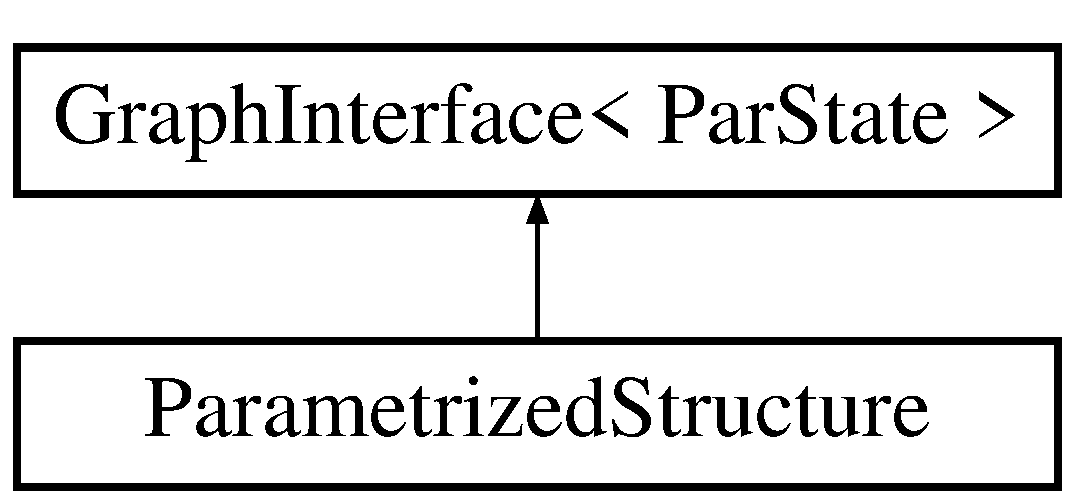
\includegraphics[height=2.000000cm]{classParametrizedStructure}
\end{center}
\end{figure}
\subsection*{\-Public \-Member \-Functions}
\begin{DoxyCompactItemize}
\item 
\hypertarget{classParametrizedStructure_a8a8fb71f58cd7ec02a05226cef4cc08b}{\hyperlink{classParametrizedStructure_a8a8fb71f58cd7ec02a05226cef4cc08b}{\-Parametrized\-Structure} ()}\label{classParametrizedStructure_a8a8fb71f58cd7ec02a05226cef4cc08b}

\begin{DoxyCompactList}\small\item\em \-Default empty constructor. \end{DoxyCompactList}\item 
const \-Levels \& \hyperlink{classParametrizedStructure_ab344a7d530e957c2ef93325863ce23a9}{get\-State\-Levels} (const \-State\-I\-D \-I\-D) const 
\item 
std\-::size\-\_\-t \hyperlink{classParametrizedStructure_aa66eea7ec82aadcb03af9c2ea9f2f289}{get\-Step\-Size} (const \-State\-I\-D \-I\-D, const std\-::size\-\_\-t transtion\-\_\-num) const 
\item 
const std\-::vector$<$ bool $>$ \& \hyperlink{classParametrizedStructure_aea25bb7c6e52090936ba18b45a169f24}{get\-Transitive} (const \-State\-I\-D \-I\-D, const std\-::size\-\_\-t transtion\-\_\-num) const 
\end{DoxyCompactItemize}
\subsection*{\-Friends}
\begin{DoxyCompactItemize}
\item 
\hypertarget{classParametrizedStructure_a6e0c14c900b776a7c27099612cffe54d}{class {\bfseries \-Parametrized\-Structure\-Builder}}\label{classParametrizedStructure_a6e0c14c900b776a7c27099612cffe54d}

\end{DoxyCompactItemize}


\subsection{\-Detailed \-Description}
\hyperlink{classParametrizedStructure}{\-Parametrized\-Structure} stores states of the \-Kripke structure created from the model together with labelled transitions. \-Each transition contains a function that causes it with explicit enumeration of values from the function that are transitive. \-To easily search for the values in the parameter bitmask, step\-\_\-size of the function is added
\begin{DoxyItemize}
\item that is the value saying how many bits of mask share the the same value for the function. \hyperlink{classParametrizedStructure}{\-Parametrized\-Structure} data can be set only from the \hyperlink{classParametrizedStructureBuilder}{\-Parametrized\-Structure\-Builder} object. 
\end{DoxyItemize}

\subsection{\-Member \-Function \-Documentation}
\hypertarget{classParametrizedStructure_ab344a7d530e957c2ef93325863ce23a9}{\index{\-Parametrized\-Structure@{\-Parametrized\-Structure}!get\-State\-Levels@{get\-State\-Levels}}
\index{get\-State\-Levels@{get\-State\-Levels}!ParametrizedStructure@{\-Parametrized\-Structure}}
\subsubsection[{get\-State\-Levels}]{\setlength{\rightskip}{0pt plus 5cm}const \-Levels\& {\bf \-Parametrized\-Structure\-::get\-State\-Levels} (
\begin{DoxyParamCaption}
\item[{const \-State\-I\-D}]{\-I\-D}
\end{DoxyParamCaption}
) const\hspace{0.3cm}{\ttfamily  \mbox{[}inline\mbox{]}}}}\label{classParametrizedStructure_ab344a7d530e957c2ef93325863ce23a9}

\begin{DoxyParams}{\-Parameters}
{\em \-I\-D} & \-I\-D of the state to get the data from\\
\hline
\end{DoxyParams}
\begin{DoxyReturn}{\-Returns}
species level 
\end{DoxyReturn}
\hypertarget{classParametrizedStructure_aa66eea7ec82aadcb03af9c2ea9f2f289}{\index{\-Parametrized\-Structure@{\-Parametrized\-Structure}!get\-Step\-Size@{get\-Step\-Size}}
\index{get\-Step\-Size@{get\-Step\-Size}!ParametrizedStructure@{\-Parametrized\-Structure}}
\subsubsection[{get\-Step\-Size}]{\setlength{\rightskip}{0pt plus 5cm}std\-::size\-\_\-t {\bf \-Parametrized\-Structure\-::get\-Step\-Size} (
\begin{DoxyParamCaption}
\item[{const \-State\-I\-D}]{\-I\-D, }
\item[{const std\-::size\-\_\-t}]{transtion\-\_\-num}
\end{DoxyParamCaption}
) const\hspace{0.3cm}{\ttfamily  \mbox{[}inline\mbox{]}}}}\label{classParametrizedStructure_aa66eea7ec82aadcb03af9c2ea9f2f289}

\begin{DoxyParams}{\-Parameters}
{\em \-I\-D} & \-I\-D of the state to get the data from \\
\hline
{\em transition\-\_\-num} & index of the transition to get the data from\\
\hline
\end{DoxyParams}
\begin{DoxyReturn}{\-Returns}
number of neighbour parameters that share the same value of the function 
\end{DoxyReturn}
\hypertarget{classParametrizedStructure_aea25bb7c6e52090936ba18b45a169f24}{\index{\-Parametrized\-Structure@{\-Parametrized\-Structure}!get\-Transitive@{get\-Transitive}}
\index{get\-Transitive@{get\-Transitive}!ParametrizedStructure@{\-Parametrized\-Structure}}
\subsubsection[{get\-Transitive}]{\setlength{\rightskip}{0pt plus 5cm}const std\-::vector$<$bool$>$\& {\bf \-Parametrized\-Structure\-::get\-Transitive} (
\begin{DoxyParamCaption}
\item[{const \-State\-I\-D}]{\-I\-D, }
\item[{const std\-::size\-\_\-t}]{transtion\-\_\-num}
\end{DoxyParamCaption}
) const\hspace{0.3cm}{\ttfamily  \mbox{[}inline\mbox{]}}}}\label{classParametrizedStructure_aea25bb7c6e52090936ba18b45a169f24}

\begin{DoxyParams}{\-Parameters}
{\em \-I\-D} & \-I\-D of the state to get the data from \\
\hline
{\em transition\-\_\-num} & index of the transition to get the data from\\
\hline
\end{DoxyParams}
\begin{DoxyReturn}{\-Returns}
target values that are includete in non-\/transitive parameters that have to be removed 
\end{DoxyReturn}


\-The documentation for this class was generated from the following file\-:\begin{DoxyCompactItemize}
\item 
construction/parametrized\-\_\-structure.\-hpp\end{DoxyCompactItemize}

\hypertarget{classParametrizedStructureBuilder}{\section{\-Parametrized\-Structure\-Builder \-Class \-Reference}
\label{classParametrizedStructureBuilder}\index{\-Parametrized\-Structure\-Builder@{\-Parametrized\-Structure\-Builder}}
}


\-Creates a \hyperlink{classParametrizedStructure}{\-Parametrized\-Structure} as a composition of a \hyperlink{classBasicStructure}{\-Basic\-Structure} and \hyperlink{classParametrizationsHolder}{\-Parametrizations\-Holder}.  




{\ttfamily \#include $<$parametrized\-\_\-structure\-\_\-builder.\-hpp$>$}

\subsection*{\-Public \-Member \-Functions}
\begin{DoxyCompactItemize}
\item 
\hyperlink{classParametrizedStructureBuilder_a61302c4c0998182eee2674887f2e7eeb}{\-Parametrized\-Structure\-Builder} (const \hyperlink{classBasicStructure}{\-Basic\-Structure} \&\-\_\-basic\-\_\-structure, const \hyperlink{classLabelingHolder}{\-Labeling\-Holder} \&\-\_\-regulatory\-\_\-functions, \hyperlink{classParametrizedStructure}{\-Parametrized\-Structure} \&\-\_\-structure)
\item 
void \hyperlink{classParametrizedStructureBuilder_ab1b302e74bd48de01243fb033abf9898}{build\-Structure} ()
\end{DoxyCompactItemize}


\subsection{\-Detailed \-Description}
\hyperlink{classParametrizedStructureBuilder}{\-Parametrized\-Structure\-Builder} creates the \hyperlink{classParametrizedStructure}{\-Parametrized\-Structure} from the model data. \-States are read from the basic structure and passed to the parametrized structure, then the transitions are added. \-Each transition is supplemented with a label -\/ mask of transitive values and the its function \-I\-D. \-This expects semantically correct data from \hyperlink{classBasicStructure}{\-Basic\-Structure} and \-Functions\-Structure. 

\subsection{\-Constructor \& \-Destructor \-Documentation}
\hypertarget{classParametrizedStructureBuilder_a61302c4c0998182eee2674887f2e7eeb}{\index{\-Parametrized\-Structure\-Builder@{\-Parametrized\-Structure\-Builder}!\-Parametrized\-Structure\-Builder@{\-Parametrized\-Structure\-Builder}}
\index{\-Parametrized\-Structure\-Builder@{\-Parametrized\-Structure\-Builder}!ParametrizedStructureBuilder@{\-Parametrized\-Structure\-Builder}}
\subsubsection[{\-Parametrized\-Structure\-Builder}]{\setlength{\rightskip}{0pt plus 5cm}\-Parametrized\-Structure\-Builder\-::\-Parametrized\-Structure\-Builder (
\begin{DoxyParamCaption}
\item[{const {\bf \-Basic\-Structure} \&}]{\-\_\-basic\-\_\-structure, }
\item[{const {\bf \-Labeling\-Holder} \&}]{\-\_\-regulatory\-\_\-functions, }
\item[{{\bf \-Parametrized\-Structure} \&}]{\-\_\-structure}
\end{DoxyParamCaption}
)\hspace{0.3cm}{\ttfamily  \mbox{[}inline\mbox{]}}}}\label{classParametrizedStructureBuilder_a61302c4c0998182eee2674887f2e7eeb}
\-Constructor just attaches the references to data holders. 

\subsection{\-Member \-Function \-Documentation}
\hypertarget{classParametrizedStructureBuilder_ab1b302e74bd48de01243fb033abf9898}{\index{\-Parametrized\-Structure\-Builder@{\-Parametrized\-Structure\-Builder}!build\-Structure@{build\-Structure}}
\index{build\-Structure@{build\-Structure}!ParametrizedStructureBuilder@{\-Parametrized\-Structure\-Builder}}
\subsubsection[{build\-Structure}]{\setlength{\rightskip}{0pt plus 5cm}void {\bf \-Parametrized\-Structure\-Builder\-::build\-Structure} (
\begin{DoxyParamCaption}
{}
\end{DoxyParamCaption}
)\hspace{0.3cm}{\ttfamily  \mbox{[}inline\mbox{]}}}}\label{classParametrizedStructureBuilder_ab1b302e74bd48de01243fb033abf9898}
\-Create the states from the model and fill the structure with them. 

\-The documentation for this class was generated from the following file\-:\begin{DoxyCompactItemize}
\item 
construction/parametrized\-\_\-structure\-\_\-builder.\-hpp\end{DoxyCompactItemize}

\hypertarget{classParamsetHelper}{\section{\-Paramset\-Helper \-Class \-Reference}
\label{classParamsetHelper}\index{\-Paramset\-Helper@{\-Paramset\-Helper}}
}


\-Class with mainly static functions for paramset (integer) handling.  




{\ttfamily \#include $<$paramset\-\_\-helper.\-hpp$>$}

\subsection*{\-Public \-Member \-Functions}
\begin{DoxyCompactItemize}
\item 
\-Paramset \hyperlink{classParamsetHelper_a010055896af6c124ead5d11f1c2851c7}{get\-All} () const 
\item 
\-Paramset \hyperlink{classParamsetHelper_a99f891518869f38c9ff5908cc3ed5283}{get\-Left\-One} (\-Color\-Num size=subset\-\_\-size) const 
\item 
std\-::vector$<$ \-Paramset $>$ \hyperlink{classParamsetHelper_a8e0b9b9b7c8088914309e865b3e2e124}{get\-Single\-Masks} (\-Paramset paramset) const 
\item 
\-Paramset \hyperlink{classParamsetHelper_aa00795ab1553c4ff7106288d19408db0}{get\-Mask\-From\-Nums} (const std\-::vector$<$ std\-::size\-\_\-t $>$ numbers) const 
\item 
\-Paramset \hyperlink{classParamsetHelper_a940010e8e14c8b42eff4640fb0c266fc}{flip} (const \-Paramset paramset) const 
\item 
\-Paramset \hyperlink{classParamsetHelper_a30f94e07f525b40f3a5704db0437b9f2}{swap} (\-Paramset paramset) const 
\item 
\-Paramset \hyperlink{classParamsetHelper_acde946486f795eda8b30aca6ab13039a}{swap} (\-Paramset paramset, const std\-::size\-\_\-t shift) const 
\item 
\hypertarget{classParamsetHelper_a84c5e76dc7b3dbbc183f97ecfe0cb472}{int {\bfseries count} (\-Paramset n) const }\label{classParamsetHelper_a84c5e76dc7b3dbbc183f97ecfe0cb472}

\item 
bool \hyperlink{classParamsetHelper_ae7c850c7f85580a73a5289ca85bf3862}{none} (\-Paramset paramset) const 
\item 
std\-::size\-\_\-t \hyperlink{classParamsetHelper_a3afd9e88dc04b9a770e0fbe9f83307a4}{get\-Bit\-Num} (\-Paramset paramset) const 
\end{DoxyCompactItemize}
\subsection*{\-Static \-Public \-Member \-Functions}
\begin{DoxyCompactItemize}
\item 
static std\-::size\-\_\-t \hyperlink{classParamsetHelper_adcdb165a22782f2dae21614f3d34b817}{get\-Paramset\-Size} ()
\end{DoxyCompactItemize}


\subsection{\-Detailed \-Description}
\-Here are methods that provide help when working with subsets of parametrization space. \begin{DoxyAttention}{\-Attention}
\-Parametrizations in an \-Paramset are ordered in an ascending order. 
\end{DoxyAttention}


\subsection{\-Member \-Function \-Documentation}
\hypertarget{classParamsetHelper_a940010e8e14c8b42eff4640fb0c266fc}{\index{\-Paramset\-Helper@{\-Paramset\-Helper}!flip@{flip}}
\index{flip@{flip}!ParamsetHelper@{\-Paramset\-Helper}}
\subsubsection[{flip}]{\setlength{\rightskip}{0pt plus 5cm}\-Paramset {\bf \-Paramset\-Helper\-::flip} (
\begin{DoxyParamCaption}
\item[{const \-Paramset}]{paramset}
\end{DoxyParamCaption}
) const\hspace{0.3cm}{\ttfamily  \mbox{[}inline\mbox{]}}}}\label{classParamsetHelper_a940010e8e14c8b42eff4640fb0c266fc}
\-Flips every bit.


\begin{DoxyParams}[1]{\-Parameters}
\mbox{\tt in}  & {\em paramset} & paramset to flip bits in\\
\hline
\end{DoxyParams}
\begin{DoxyReturn}{\-Returns}
copy of input with swapped bits. 
\end{DoxyReturn}
\hypertarget{classParamsetHelper_a010055896af6c124ead5d11f1c2851c7}{\index{\-Paramset\-Helper@{\-Paramset\-Helper}!get\-All@{get\-All}}
\index{get\-All@{get\-All}!ParamsetHelper@{\-Paramset\-Helper}}
\subsubsection[{get\-All}]{\setlength{\rightskip}{0pt plus 5cm}\-Paramset {\bf \-Paramset\-Helper\-::get\-All} (
\begin{DoxyParamCaption}
{}
\end{DoxyParamCaption}
) const\hspace{0.3cm}{\ttfamily  \mbox{[}inline\mbox{]}}}}\label{classParamsetHelper_a010055896af6c124ead5d11f1c2851c7}
\begin{DoxyReturn}{\-Returns}
paramset with everything set to 1 
\end{DoxyReturn}
\hypertarget{classParamsetHelper_a3afd9e88dc04b9a770e0fbe9f83307a4}{\index{\-Paramset\-Helper@{\-Paramset\-Helper}!get\-Bit\-Num@{get\-Bit\-Num}}
\index{get\-Bit\-Num@{get\-Bit\-Num}!ParamsetHelper@{\-Paramset\-Helper}}
\subsubsection[{get\-Bit\-Num}]{\setlength{\rightskip}{0pt plus 5cm}std\-::size\-\_\-t {\bf \-Paramset\-Helper\-::get\-Bit\-Num} (
\begin{DoxyParamCaption}
\item[{\-Paramset}]{paramset}
\end{DoxyParamCaption}
) const\hspace{0.3cm}{\ttfamily  \mbox{[}inline\mbox{]}}}}\label{classParamsetHelper_a3afd9e88dc04b9a770e0fbe9f83307a4}
\-Get a number of the first on bit.


\begin{DoxyParams}[1]{\-Parameters}
\mbox{\tt in}  & {\em paramset} & bitmask that is required to have just one bit on\\
\hline
\end{DoxyParams}
\begin{DoxyReturn}{\-Returns}
position of the bit in the mask (from the left) 
\end{DoxyReturn}
\hypertarget{classParamsetHelper_a99f891518869f38c9ff5908cc3ed5283}{\index{\-Paramset\-Helper@{\-Paramset\-Helper}!get\-Left\-One@{get\-Left\-One}}
\index{get\-Left\-One@{get\-Left\-One}!ParamsetHelper@{\-Paramset\-Helper}}
\subsubsection[{get\-Left\-One}]{\setlength{\rightskip}{0pt plus 5cm}\-Paramset {\bf \-Paramset\-Helper\-::get\-Left\-One} (
\begin{DoxyParamCaption}
\item[{\-Color\-Num}]{size = {\ttfamily subset\-\_\-size}}
\end{DoxyParamCaption}
) const\hspace{0.3cm}{\ttfamily  \mbox{[}inline\mbox{]}}}}\label{classParamsetHelper_a99f891518869f38c9ff5908cc3ed5283}
\begin{DoxyReturn}{\-Returns}
paramset that holds value of the binary form 10...0 (leftmost parametrization) 
\end{DoxyReturn}
\hypertarget{classParamsetHelper_aa00795ab1553c4ff7106288d19408db0}{\index{\-Paramset\-Helper@{\-Paramset\-Helper}!get\-Mask\-From\-Nums@{get\-Mask\-From\-Nums}}
\index{get\-Mask\-From\-Nums@{get\-Mask\-From\-Nums}!ParamsetHelper@{\-Paramset\-Helper}}
\subsubsection[{get\-Mask\-From\-Nums}]{\setlength{\rightskip}{0pt plus 5cm}\-Paramset {\bf \-Paramset\-Helper\-::get\-Mask\-From\-Nums} (
\begin{DoxyParamCaption}
\item[{const std\-::vector$<$ std\-::size\-\_\-t $>$}]{numbers}
\end{DoxyParamCaption}
) const\hspace{0.3cm}{\ttfamily  \mbox{[}inline\mbox{]}}}}\label{classParamsetHelper_aa00795ab1553c4ff7106288d19408db0}
\-Return a paramset with on bits corresponding to requested numbers -\/ i.\-e. for \{1,3\} we would get 1010...0.


\begin{DoxyParams}[1]{\-Parameters}
\mbox{\tt in}  & {\em vector} & of number in range \mbox{[}1,$|$paramset$|$\mbox{]}\\
\hline
\end{DoxyParams}
\begin{DoxyReturn}{\-Returns}
\-Paramset mask 
\end{DoxyReturn}
\hypertarget{classParamsetHelper_adcdb165a22782f2dae21614f3d34b817}{\index{\-Paramset\-Helper@{\-Paramset\-Helper}!get\-Paramset\-Size@{get\-Paramset\-Size}}
\index{get\-Paramset\-Size@{get\-Paramset\-Size}!ParamsetHelper@{\-Paramset\-Helper}}
\subsubsection[{get\-Paramset\-Size}]{\setlength{\rightskip}{0pt plus 5cm}static std\-::size\-\_\-t {\bf \-Paramset\-Helper\-::get\-Paramset\-Size} (
\begin{DoxyParamCaption}
{}
\end{DoxyParamCaption}
)\hspace{0.3cm}{\ttfamily  \mbox{[}inline, static\mbox{]}}}}\label{classParamsetHelper_adcdb165a22782f2dae21614f3d34b817}
\-V\-A\-L\-U\-E \-G\-E\-T\-T\-E\-R\-S \begin{DoxyReturn}{\-Returns}
number of parametrizations in a single round 
\end{DoxyReturn}
\hypertarget{classParamsetHelper_a8e0b9b9b7c8088914309e865b3e2e124}{\index{\-Paramset\-Helper@{\-Paramset\-Helper}!get\-Single\-Masks@{get\-Single\-Masks}}
\index{get\-Single\-Masks@{get\-Single\-Masks}!ParamsetHelper@{\-Paramset\-Helper}}
\subsubsection[{get\-Single\-Masks}]{\setlength{\rightskip}{0pt plus 5cm}std\-::vector$<$\-Paramset$>$ {\bf \-Paramset\-Helper\-::get\-Single\-Masks} (
\begin{DoxyParamCaption}
\item[{\-Paramset}]{paramset}
\end{DoxyParamCaption}
) const\hspace{0.3cm}{\ttfamily  \mbox{[}inline\mbox{]}}}}\label{classParamsetHelper_a8e0b9b9b7c8088914309e865b3e2e124}
\-T\-R\-A\-N\-S\-F\-O\-R\-M\-E\-R\-S \-Computer a vector of masks of single parametrizations -\/ i.\-e. 10010 would give \{10000,00010\}.


\begin{DoxyParams}[1]{\-Parameters}
\mbox{\tt in}  & {\em paramset} & paramset to disassamble\\
\hline
\end{DoxyParams}
\begin{DoxyReturn}{\-Returns}
vector containing a paramset with a single parametrization for each parametrization in input paramset 
\end{DoxyReturn}
\hypertarget{classParamsetHelper_ae7c850c7f85580a73a5289ca85bf3862}{\index{\-Paramset\-Helper@{\-Paramset\-Helper}!none@{none}}
\index{none@{none}!ParamsetHelper@{\-Paramset\-Helper}}
\subsubsection[{none}]{\setlength{\rightskip}{0pt plus 5cm}bool {\bf \-Paramset\-Helper\-::none} (
\begin{DoxyParamCaption}
\item[{\-Paramset}]{paramset}
\end{DoxyParamCaption}
) const\hspace{0.3cm}{\ttfamily  \mbox{[}inline\mbox{]}}}}\label{classParamsetHelper_ae7c850c7f85580a73a5289ca85bf3862}
\-Test if none of the parametrizations is present.


\begin{DoxyParams}[1]{\-Parameters}
\mbox{\tt in}  & {\em paramset} & paramset to count bits in\\
\hline
\end{DoxyParams}
\begin{DoxyReturn}{\-Returns}
true if none of the paremters is set 
\end{DoxyReturn}
\hypertarget{classParamsetHelper_a30f94e07f525b40f3a5704db0437b9f2}{\index{\-Paramset\-Helper@{\-Paramset\-Helper}!swap@{swap}}
\index{swap@{swap}!ParamsetHelper@{\-Paramset\-Helper}}
\subsubsection[{swap}]{\setlength{\rightskip}{0pt plus 5cm}\-Paramset {\bf \-Paramset\-Helper\-::swap} (
\begin{DoxyParamCaption}
\item[{\-Paramset}]{paramset}
\end{DoxyParamCaption}
) const\hspace{0.3cm}{\ttfamily  \mbox{[}inline\mbox{]}}}}\label{classParamsetHelper_a30f94e07f525b40f3a5704db0437b9f2}
\-Swaps paramset within a variable -\/ last become first etc.


\begin{DoxyParams}[1]{\-Parameters}
\mbox{\tt in}  & {\em paramset} & paramset to swap bits in\\
\hline
\end{DoxyParams}
\begin{DoxyReturn}{\-Returns}
copy of input with descending order of paramset 
\end{DoxyReturn}
\hypertarget{classParamsetHelper_acde946486f795eda8b30aca6ab13039a}{\index{\-Paramset\-Helper@{\-Paramset\-Helper}!swap@{swap}}
\index{swap@{swap}!ParamsetHelper@{\-Paramset\-Helper}}
\subsubsection[{swap}]{\setlength{\rightskip}{0pt plus 5cm}\-Paramset {\bf \-Paramset\-Helper\-::swap} (
\begin{DoxyParamCaption}
\item[{\-Paramset}]{paramset, }
\item[{const std\-::size\-\_\-t}]{shift}
\end{DoxyParamCaption}
) const\hspace{0.3cm}{\ttfamily  \mbox{[}inline\mbox{]}}}}\label{classParamsetHelper_acde946486f795eda8b30aca6ab13039a}
\-Swaps paramset within a variable -\/ last become first etc.


\begin{DoxyParams}[1]{\-Parameters}
\mbox{\tt in}  & {\em paramset} & paramset to swap bits in \\
\hline
\mbox{\tt in}  & {\em shift} & if there are not all the paramset used, shift back after swapping\\
\hline
\end{DoxyParams}
\begin{DoxyReturn}{\-Returns}
copy of input with descending order of paramset 
\end{DoxyReturn}


\-The documentation for this class was generated from the following file\-:\begin{DoxyCompactItemize}
\item 
synthesis/paramset\-\_\-helper.\-hpp\end{DoxyCompactItemize}

\hypertarget{classParsingManager}{\section{\-Parsing\-Manager \-Class \-Reference}
\label{classParsingManager}\index{\-Parsing\-Manager@{\-Parsing\-Manager}}
}


\-S\-T\-E\-P 1 -\/ \-Class that manages all of the parsing done by the application. \-Includes parsing of arguments and parsing of models.  




{\ttfamily \#include $<$parsing\-\_\-manager.\-hpp$>$}

\subsection*{\-Public \-Member \-Functions}
\begin{DoxyCompactItemize}
\item 
\hyperlink{classParsingManager_a85070bf191f8a33eb08e9bdbfb10bdfb}{\-Parsing\-Manager} (int argc, char $\ast$argv\mbox{[}$\,$\mbox{]}, \hyperlink{classModel}{\-Model} \&\-\_\-model)
\item 
void \hyperlink{classParsingManager_a7865623b21a0bde40a63b8b0b6bd6862}{parse} ()
\end{DoxyCompactItemize}


\subsection{\-Constructor \& \-Destructor \-Documentation}
\hypertarget{classParsingManager_a85070bf191f8a33eb08e9bdbfb10bdfb}{\index{\-Parsing\-Manager@{\-Parsing\-Manager}!\-Parsing\-Manager@{\-Parsing\-Manager}}
\index{\-Parsing\-Manager@{\-Parsing\-Manager}!ParsingManager@{\-Parsing\-Manager}}
\subsubsection[{\-Parsing\-Manager}]{\setlength{\rightskip}{0pt plus 5cm}\-Parsing\-Manager\-::\-Parsing\-Manager (
\begin{DoxyParamCaption}
\item[{int}]{argc, }
\item[{char $\ast$}]{argv\mbox{[}$\,$\mbox{]}, }
\item[{{\bf \-Model} \&}]{\-\_\-model}
\end{DoxyParamCaption}
)\hspace{0.3cm}{\ttfamily  \mbox{[}inline\mbox{]}}}}\label{classParsingManager_a85070bf191f8a33eb08e9bdbfb10bdfb}
\-Constructor copies arguments from the argv and passes the model object that will store parsed information.


\begin{DoxyParams}{\-Parameters}
{\em argc} & passed argc from main() \\
\hline
{\em argv} & passed argv from main() \\
\hline
{\em \-\_\-model} & model storing the reference data \\
\hline
\end{DoxyParams}


\subsection{\-Member \-Function \-Documentation}
\hypertarget{classParsingManager_a7865623b21a0bde40a63b8b0b6bd6862}{\index{\-Parsing\-Manager@{\-Parsing\-Manager}!parse@{parse}}
\index{parse@{parse}!ParsingManager@{\-Parsing\-Manager}}
\subsubsection[{parse}]{\setlength{\rightskip}{0pt plus 5cm}void {\bf \-Parsing\-Manager\-::parse} (
\begin{DoxyParamCaption}
{}
\end{DoxyParamCaption}
)\hspace{0.3cm}{\ttfamily  \mbox{[}inline\mbox{]}}}}\label{classParsingManager_a7865623b21a0bde40a63b8b0b6bd6862}
\-Main parsing function. 

\-The documentation for this class was generated from the following file\-:\begin{DoxyCompactItemize}
\item 
parsing/parsing\-\_\-manager.\-hpp\end{DoxyCompactItemize}

\hypertarget{structParState}{\section{\-Par\-State \-Struct \-Reference}
\label{structParState}\index{\-Par\-State@{\-Par\-State}}
}


\-Simple state enriched with transition functions.  




{\ttfamily \#include $<$parametrized\-\_\-structure.\-hpp$>$}

\-Inheritance diagram for \-Par\-State\-:\begin{figure}[H]
\begin{center}
\leavevmode
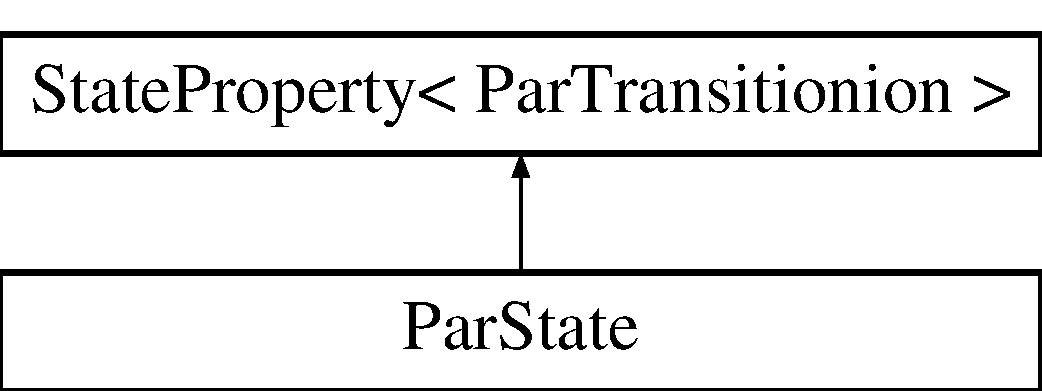
\includegraphics[height=2.000000cm]{structParState}
\end{center}
\end{figure}
\subsection*{\-Public \-Member \-Functions}
\begin{DoxyCompactItemize}
\item 
\hypertarget{structParState_ae4e91ec8c56886293d00718cd0756fe0}{\hyperlink{structParState_ae4e91ec8c56886293d00718cd0756fe0}{\-Par\-State} (const \-State\-I\-D \hyperlink{structStateProperty_af33be20c9033f9b6524c0447e7ac647e}{\-I\-D}, const \-Levels \&\-\_\-species\-\_\-level, const std\-::string \&\&\hyperlink{structStateProperty_a7cfb634f80b68196eefa54e8ee98a5fe}{label})}\label{structParState_ae4e91ec8c56886293d00718cd0756fe0}

\begin{DoxyCompactList}\small\item\em \-Simple filler, assigns values to all the variables. \end{DoxyCompactList}\end{DoxyCompactItemize}
\subsection*{\-Public \-Attributes}
\begin{DoxyCompactItemize}
\item 
\hypertarget{structParState_a5f55f29ca601e3fe84f42c52a26f14de}{\-Levels \hyperlink{structParState_a5f55f29ca601e3fe84f42c52a26f14de}{species\-\_\-level}}\label{structParState_a5f55f29ca601e3fe84f42c52a26f14de}

\begin{DoxyCompactList}\small\item\em \-Species\-\_\-level\mbox{[}i\mbox{]} = activation level of specie i. \end{DoxyCompactList}\end{DoxyCompactItemize}


\-The documentation for this struct was generated from the following file\-:\begin{DoxyCompactItemize}
\item 
construction/parametrized\-\_\-structure.\-hpp\end{DoxyCompactItemize}

\hypertarget{structParTransitionion}{\section{\-Par\-Transitionion \-Struct \-Reference}
\label{structParTransitionion}\index{\-Par\-Transitionion@{\-Par\-Transitionion}}
}


\-Storing a single transition to neighbour state together with its transition function.  




{\ttfamily \#include $<$parametrized\-\_\-structure.\-hpp$>$}

\-Inheritance diagram for \-Par\-Transitionion\-:\begin{figure}[H]
\begin{center}
\leavevmode
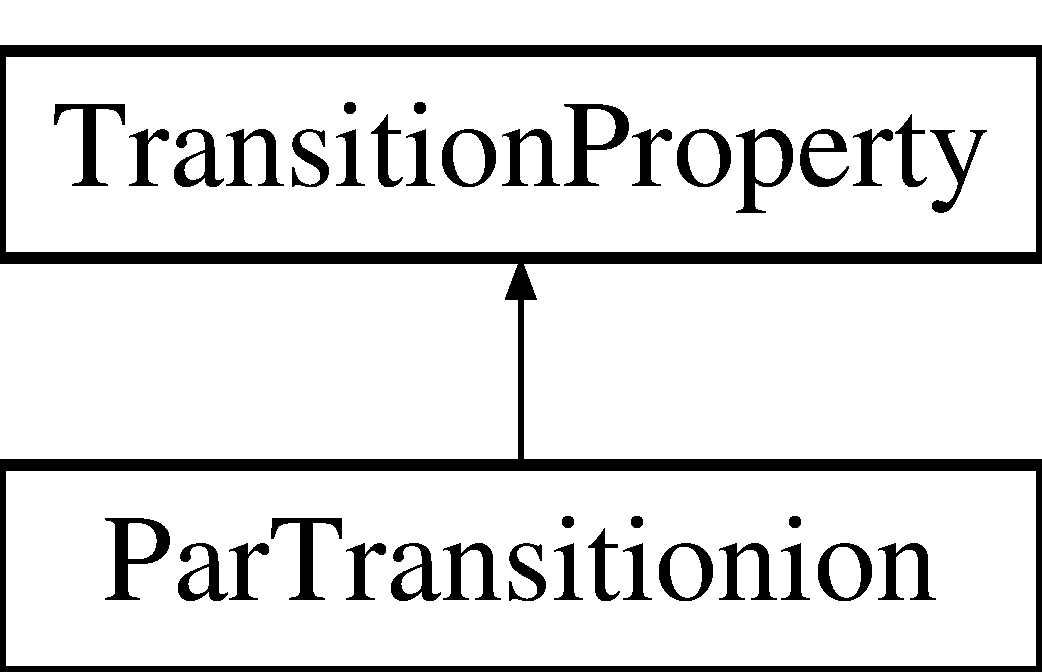
\includegraphics[height=2.000000cm]{structParTransitionion}
\end{center}
\end{figure}
\subsection*{\-Public \-Member \-Functions}
\begin{DoxyCompactItemize}
\item 
\hypertarget{structParTransitionion_abf024116d00c3e74fd326d433647024c}{\hyperlink{structParTransitionion_abf024116d00c3e74fd326d433647024c}{\-Par\-Transitionion} (const \-State\-I\-D \hyperlink{structTransitionProperty_a1e272cf5a26a0db442ac0fed5b797386}{target\-\_\-\-I\-D}, const std\-::size\-\_\-t \-\_\-step\-\_\-size, std\-::vector$<$ bool $>$ \&\&\-\_\-transitive\-\_\-values)}\label{structParTransitionion_abf024116d00c3e74fd326d433647024c}

\begin{DoxyCompactList}\small\item\em \-Simple filler, assigns values to all the variables. \end{DoxyCompactList}\end{DoxyCompactItemize}
\subsection*{\-Public \-Attributes}
\begin{DoxyCompactItemize}
\item 
\hypertarget{structParTransitionion_a9855b275a397fd29b91ac6b353a648b8}{std\-::size\-\_\-t \hyperlink{structParTransitionion_a9855b275a397fd29b91ac6b353a648b8}{step\-\_\-size}}\label{structParTransitionion_a9855b275a397fd29b91ac6b353a648b8}

\begin{DoxyCompactList}\small\item\em \-How many bits of a parameter space bitset is needed to get from one targe value to another. \end{DoxyCompactList}\item 
\hypertarget{structParTransitionion_a2ec3aaad7a34245ac07c52523697a584}{std\-::vector$<$ bool $>$ \hyperlink{structParTransitionion_a2ec3aaad7a34245ac07c52523697a584}{transitive\-\_\-values}}\label{structParTransitionion_a2ec3aaad7a34245ac07c52523697a584}

\begin{DoxyCompactList}\small\item\em \-Which values from the original set does not allow a trasition and therefore removes bits from the mask. \end{DoxyCompactList}\end{DoxyCompactItemize}


\-The documentation for this struct was generated from the following file\-:\begin{DoxyCompactItemize}
\item 
construction/parametrized\-\_\-structure.\-hpp\end{DoxyCompactItemize}

\hypertarget{structProdState}{\section{\-Prod\-State \-Struct \-Reference}
\label{structProdState}\index{\-Prod\-State@{\-Prod\-State}}
}


\-State of the product -\/ same as the state of parametrized structure but put together with a \-B\-A state.  




{\ttfamily \#include $<$product\-\_\-structure.\-hpp$>$}

\-Inheritance diagram for \-Prod\-State\-:\begin{figure}[H]
\begin{center}
\leavevmode
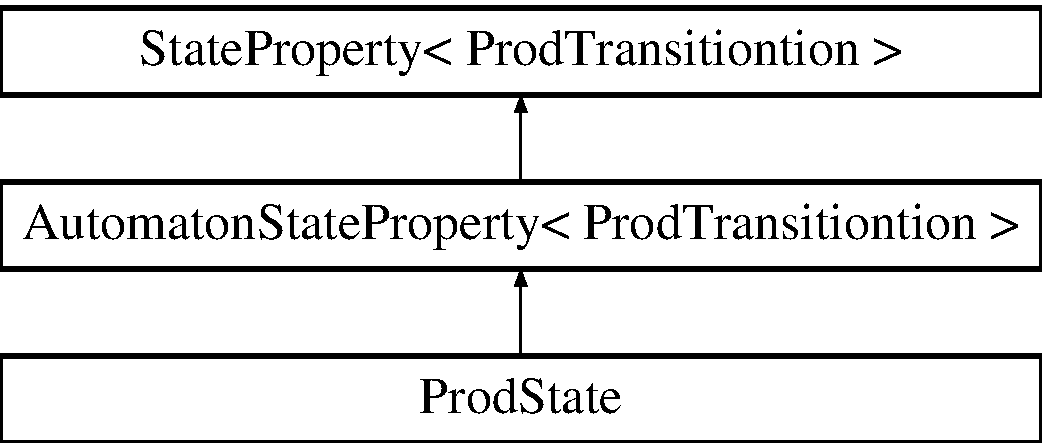
\includegraphics[height=3.000000cm]{structProdState}
\end{center}
\end{figure}
\subsection*{\-Public \-Member \-Functions}
\begin{DoxyCompactItemize}
\item 
\hypertarget{structProdState_a4a3330daa5026f94e302e61f58e41521}{\hyperlink{structProdState_a4a3330daa5026f94e302e61f58e41521}{\-Prod\-State} (const \-State\-I\-D \hyperlink{structStateProperty_af33be20c9033f9b6524c0447e7ac647e}{\-I\-D}, const std\-::string \&\&\hyperlink{structStateProperty_a7cfb634f80b68196eefa54e8ee98a5fe}{label}, const \-State\-I\-D \-\_\-\-K\-S\-\_\-\-I\-D, const \-State\-I\-D \-\_\-\-B\-A\-\_\-\-I\-D, const bool \hyperlink{structAutomatonStateProperty_a01c05b93d68d3f72b76ab9835abc5476}{initial}, const bool \hyperlink{structAutomatonStateProperty_aa95898834a149d202575a6f655a5e5e2}{final}, const \-Levels \&\-\_\-species\-\_\-level)}\label{structProdState_a4a3330daa5026f94e302e61f58e41521}

\begin{DoxyCompactList}\small\item\em \-Simple filler, assigns values to all the variables. \end{DoxyCompactList}\end{DoxyCompactItemize}
\subsection*{\-Public \-Attributes}
\begin{DoxyCompactItemize}
\item 
\hypertarget{structProdState_ae3e8c419af83f5f2c1d5eeae9ea1f7d4}{\-State\-I\-D \hyperlink{structProdState_ae3e8c419af83f5f2c1d5eeae9ea1f7d4}{\-K\-S\-\_\-\-I\-D}}\label{structProdState_ae3e8c419af83f5f2c1d5eeae9ea1f7d4}

\begin{DoxyCompactList}\small\item\em \-I\-D of an original \-K\-S state this one is built from. \end{DoxyCompactList}\item 
\hypertarget{structProdState_a6943a6a8d360ed3cc9bfa831259dc668}{\-State\-I\-D \hyperlink{structProdState_a6943a6a8d360ed3cc9bfa831259dc668}{\-B\-A\-\_\-\-I\-D}}\label{structProdState_a6943a6a8d360ed3cc9bfa831259dc668}

\begin{DoxyCompactList}\small\item\em \-I\-D of an original \-B\-A state this one is built from. \end{DoxyCompactList}\item 
\hypertarget{structProdState_ad8d5b69a4dea4a5fe1a3adbf949f38c5}{\-Levels \hyperlink{structProdState_ad8d5b69a4dea4a5fe1a3adbf949f38c5}{species\-\_\-level}}\label{structProdState_ad8d5b69a4dea4a5fe1a3adbf949f38c5}

\begin{DoxyCompactList}\small\item\em species\-\_\-level\mbox{[}i\mbox{]} = activation level of specie i in this state \end{DoxyCompactList}\end{DoxyCompactItemize}


\-The documentation for this struct was generated from the following file\-:\begin{DoxyCompactItemize}
\item 
construction/product\-\_\-structure.\-hpp\end{DoxyCompactItemize}

\hypertarget{structProdTransitiontion}{\section{\-Prod\-Transitiontion \-Struct \-Reference}
\label{structProdTransitiontion}\index{\-Prod\-Transitiontion@{\-Prod\-Transitiontion}}
}


\-Storing a single transition to a neighbour state together with its transition function.  




{\ttfamily \#include $<$product\-\_\-structure.\-hpp$>$}

\-Inheritance diagram for \-Prod\-Transitiontion\-:\begin{figure}[H]
\begin{center}
\leavevmode
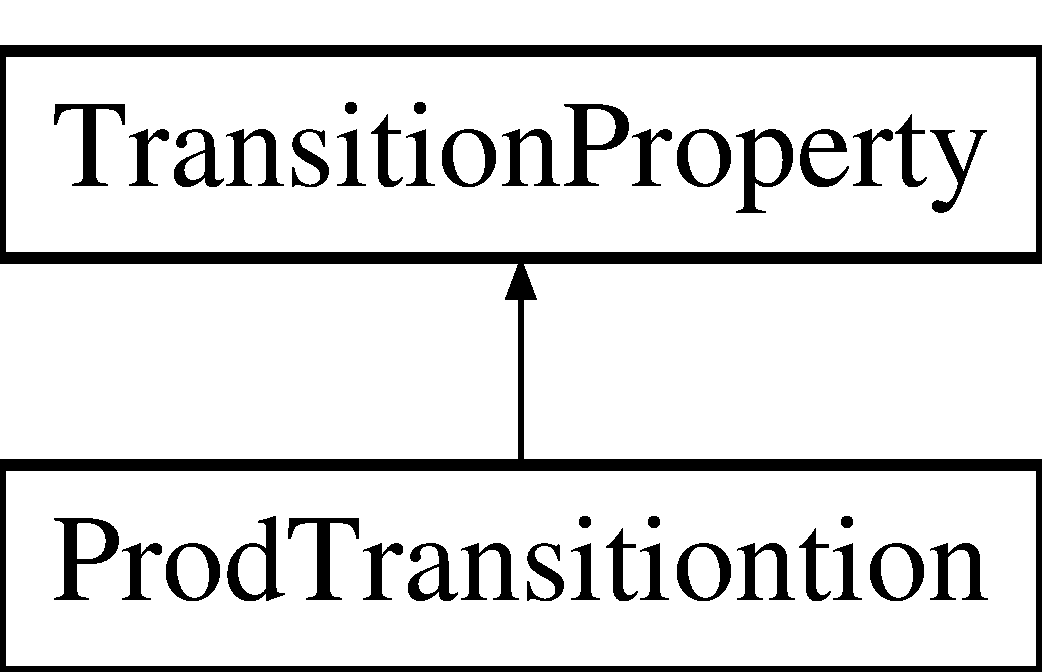
\includegraphics[height=2.000000cm]{structProdTransitiontion}
\end{center}
\end{figure}
\subsection*{\-Public \-Member \-Functions}
\begin{DoxyCompactItemize}
\item 
\hypertarget{structProdTransitiontion_aa349b7a418a751f818175eb0f73eac17}{\hyperlink{structProdTransitiontion_aa349b7a418a751f818175eb0f73eac17}{\-Prod\-Transitiontion} (const \-State\-I\-D \hyperlink{structTransitionProperty_a1e272cf5a26a0db442ac0fed5b797386}{target\-\_\-\-I\-D}, const std\-::size\-\_\-t \-\_\-step\-\_\-size, const std\-::vector$<$ bool $>$ \&\-\_\-transitive\-\_\-values)}\label{structProdTransitiontion_aa349b7a418a751f818175eb0f73eac17}

\begin{DoxyCompactList}\small\item\em \-Simple filler, assigns values to all the variables. \end{DoxyCompactList}\end{DoxyCompactItemize}
\subsection*{\-Public \-Attributes}
\begin{DoxyCompactItemize}
\item 
\hypertarget{structProdTransitiontion_ad8491d31e0abb07dd7a4b61b04ed757d}{std\-::size\-\_\-t \hyperlink{structProdTransitiontion_ad8491d31e0abb07dd7a4b61b04ed757d}{step\-\_\-size}}\label{structProdTransitiontion_ad8491d31e0abb07dd7a4b61b04ed757d}

\begin{DoxyCompactList}\small\item\em \-How many bits of a parameter space bitset is needed to get from one targe value to another. \end{DoxyCompactList}\item 
\hypertarget{structProdTransitiontion_a2048f6226ba33b7800ab15986116fd6a}{std\-::vector$<$ bool $>$ \hyperlink{structProdTransitiontion_a2048f6226ba33b7800ab15986116fd6a}{transitive\-\_\-values}}\label{structProdTransitiontion_a2048f6226ba33b7800ab15986116fd6a}

\begin{DoxyCompactList}\small\item\em \-Which values from the original set does not allow a trasition and therefore removes bits from the mask. \end{DoxyCompactList}\end{DoxyCompactItemize}


\-The documentation for this struct was generated from the following file\-:\begin{DoxyCompactItemize}
\item 
construction/product\-\_\-structure.\-hpp\end{DoxyCompactItemize}

\hypertarget{classProductBuilder}{\section{\-Product\-Builder \-Class \-Reference}
\label{classProductBuilder}\index{\-Product\-Builder@{\-Product\-Builder}}
}


\-Creates a final \hyperlink{classProductStructure}{\-Product\-Structure} that is used as a template for the synthesis procedure, as a product of \hyperlink{classParametrizedStructure}{\-Parametrized\-Structure} and \hyperlink{classAutomatonStructure}{\-Automaton\-Structure}.  




{\ttfamily \#include $<$product\-\_\-builder.\-hpp$>$}

\subsection*{\-Public \-Member \-Functions}
\begin{DoxyCompactItemize}
\item 
\hyperlink{classProductBuilder_a43533c506209311b76fa7cd8c216ea5f}{\-Product\-Builder} (const \hyperlink{classParametrizedStructure}{\-Parametrized\-Structure} \&\-\_\-structure, const \hyperlink{classAutomatonStructure}{\-Automaton\-Structure} \&\-\_\-automaton, \hyperlink{classProductStructure}{\-Product\-Structure} \&\-\_\-product)
\item 
void \hyperlink{classProductBuilder_a1eaedceb9c2d2bff07090abfa82d83dd}{build\-Product} ()
\end{DoxyCompactItemize}


\subsection{\-Detailed \-Description}
\hyperlink{classProductBuilder}{\-Product\-Builder} creates the an automaton corresponding to the synchronous product of \-B\-A and \-K\-S. \begin{DoxyAttention}{\-Attention}
\-States of product are indexed as (\-B\-A\-\_\-state\-\_\-count $\ast$ \-K\-S\-\_\-state\-\_\-\-I\-D + \-B\-A\-\_\-state\-\_\-\-I\-D) -\/ e.\-g. if 3-\/state \-B\-A state ((1,0)x(1)) would be at position 3$\ast$1 + 1 = 4. 
\end{DoxyAttention}


\subsection{\-Constructor \& \-Destructor \-Documentation}
\hypertarget{classProductBuilder_a43533c506209311b76fa7cd8c216ea5f}{\index{\-Product\-Builder@{\-Product\-Builder}!\-Product\-Builder@{\-Product\-Builder}}
\index{\-Product\-Builder@{\-Product\-Builder}!ProductBuilder@{\-Product\-Builder}}
\subsubsection[{\-Product\-Builder}]{\setlength{\rightskip}{0pt plus 5cm}\-Product\-Builder\-::\-Product\-Builder (
\begin{DoxyParamCaption}
\item[{const {\bf \-Parametrized\-Structure} \&}]{\-\_\-structure, }
\item[{const {\bf \-Automaton\-Structure} \&}]{\-\_\-automaton, }
\item[{{\bf \-Product\-Structure} \&}]{\-\_\-product}
\end{DoxyParamCaption}
)\hspace{0.3cm}{\ttfamily  \mbox{[}inline\mbox{]}}}}\label{classProductBuilder_a43533c506209311b76fa7cd8c216ea5f}
\-Constructor just attaches the references of data holders. 

\subsection{\-Member \-Function \-Documentation}
\hypertarget{classProductBuilder_a1eaedceb9c2d2bff07090abfa82d83dd}{\index{\-Product\-Builder@{\-Product\-Builder}!build\-Product@{build\-Product}}
\index{build\-Product@{build\-Product}!ProductBuilder@{\-Product\-Builder}}
\subsubsection[{build\-Product}]{\setlength{\rightskip}{0pt plus 5cm}void {\bf \-Product\-Builder\-::build\-Product} (
\begin{DoxyParamCaption}
{}
\end{DoxyParamCaption}
)\hspace{0.3cm}{\ttfamily  \mbox{[}inline\mbox{]}}}}\label{classProductBuilder_a1eaedceb9c2d2bff07090abfa82d83dd}
\-Create the the synchronous product of the provided \-B\-A and \-P\-K\-S. 

\-The documentation for this class was generated from the following file\-:\begin{DoxyCompactItemize}
\item 
construction/product\-\_\-builder.\-hpp\end{DoxyCompactItemize}

\hypertarget{classProductStructure}{\section{\-Product\-Structure \-Class \-Reference}
\label{classProductStructure}\index{\-Product\-Structure@{\-Product\-Structure}}
}


\-Holds a product structure -\/ the one that is used in coloring procedure.  




{\ttfamily \#include $<$product\-\_\-structure.\-hpp$>$}

\-Inheritance diagram for \-Product\-Structure\-:\begin{figure}[H]
\begin{center}
\leavevmode
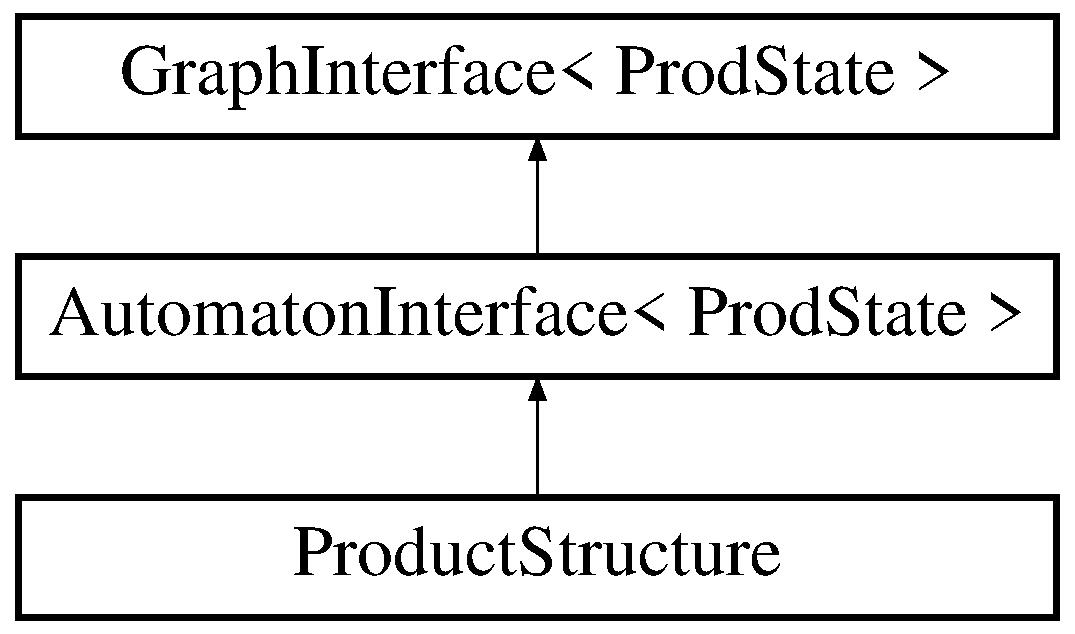
\includegraphics[height=3.000000cm]{classProductStructure}
\end{center}
\end{figure}
\subsection*{\-Public \-Member \-Functions}
\begin{DoxyCompactItemize}
\item 
\hypertarget{classProductStructure_a1669ec333c66cc802ba2a5f781e4dd41}{\hyperlink{classProductStructure_a1669ec333c66cc802ba2a5f781e4dd41}{\-Product\-Structure} (const \hyperlink{classParametrizedStructure}{\-Parametrized\-Structure} \&\-\_\-structure, const \hyperlink{classAutomatonStructure}{\-Automaton\-Structure} \&\-\_\-automaton)}\label{classProductStructure_a1669ec333c66cc802ba2a5f781e4dd41}

\begin{DoxyCompactList}\small\item\em \-Default constructor, only passes the data. \end{DoxyCompactList}\item 
\-State\-I\-D \hyperlink{classProductStructure_abc8e244f4cdeaff7bcea7f592a4b2297}{get\-Product\-I\-D} (const \-State\-I\-D \-K\-S\-\_\-\-I\-D, const \-State\-I\-D \-B\-A\-\_\-\-I\-D) const 
\item 
\-State\-I\-D \hyperlink{classProductStructure_ad5c76b37b08e6aac431624c229a83958}{get\-B\-A\-I\-D} (const \-State\-I\-D \-I\-D) const 
\item 
\-State\-I\-D \hyperlink{classProductStructure_a650c655568c984ec1138f91691693a15}{get\-K\-S\-I\-D} (const \-State\-I\-D \-I\-D) const 
\item 
const \-Levels \& \hyperlink{classProductStructure_ae55a35958534cebb974d491ff80fedc1}{get\-State\-Levels} (const \-State\-I\-D \-I\-D) const 
\item 
std\-::size\-\_\-t \hyperlink{classProductStructure_ae6905f6bedffcb40115a9ddd2edb1d5a}{get\-Step\-Size} (const \-State\-I\-D \-I\-D, const std\-::size\-\_\-t transtion\-\_\-num) const 
\item 
const std\-::vector$<$ bool $>$ \& \hyperlink{classProductStructure_a0b4ed666548d34270779222d4ae31606}{get\-Transitive} (const \-State\-I\-D \-I\-D, const std\-::size\-\_\-t transtion\-\_\-num) const 
\end{DoxyCompactItemize}
\subsection*{\-Friends}
\begin{DoxyCompactItemize}
\item 
\hypertarget{classProductStructure_a6c45ddd297f18174168e322ae1b74396}{class {\bfseries \-Product\-Builder}}\label{classProductStructure_a6c45ddd297f18174168e322ae1b74396}

\end{DoxyCompactItemize}


\subsection{\-Detailed \-Description}
\-This is the final step of construction -\/ a structure that is acutally used during the computation. \-For simplicity, it copies data from its predecessors (\-B\-A and \-P\-K\-S). \begin{DoxyAttention}{\-Attention}
\-States of product are indexed as (\-B\-A\-\_\-state\-\_\-count $\ast$ \-K\-S\-\_\-state\-\_\-\-I\-D + \-B\-A\-\_\-state\-\_\-\-I\-D) -\/ e.\-g. if 3-\/state \-B\-A state ((1,0)x(1)) would be at position 3$\ast$1 + 1 = 4.
\end{DoxyAttention}
\hyperlink{classProductStructure}{\-Product\-Structure} data can be set only from the \hyperlink{classProductBuilder}{\-Product\-Builder} object. 

\subsection{\-Member \-Function \-Documentation}
\hypertarget{classProductStructure_ad5c76b37b08e6aac431624c229a83958}{\index{\-Product\-Structure@{\-Product\-Structure}!get\-B\-A\-I\-D@{get\-B\-A\-I\-D}}
\index{get\-B\-A\-I\-D@{get\-B\-A\-I\-D}!ProductStructure@{\-Product\-Structure}}
\subsubsection[{get\-B\-A\-I\-D}]{\setlength{\rightskip}{0pt plus 5cm}\-State\-I\-D {\bf \-Product\-Structure\-::get\-B\-A\-I\-D} (
\begin{DoxyParamCaption}
\item[{const \-State\-I\-D}]{\-I\-D}
\end{DoxyParamCaption}
) const\hspace{0.3cm}{\ttfamily  \mbox{[}inline\mbox{]}}}}\label{classProductStructure_ad5c76b37b08e6aac431624c229a83958}
\begin{DoxyReturn}{\-Returns}
index of \-B\-A state form the product 
\end{DoxyReturn}
\hypertarget{classProductStructure_a650c655568c984ec1138f91691693a15}{\index{\-Product\-Structure@{\-Product\-Structure}!get\-K\-S\-I\-D@{get\-K\-S\-I\-D}}
\index{get\-K\-S\-I\-D@{get\-K\-S\-I\-D}!ProductStructure@{\-Product\-Structure}}
\subsubsection[{get\-K\-S\-I\-D}]{\setlength{\rightskip}{0pt plus 5cm}\-State\-I\-D {\bf \-Product\-Structure\-::get\-K\-S\-I\-D} (
\begin{DoxyParamCaption}
\item[{const \-State\-I\-D}]{\-I\-D}
\end{DoxyParamCaption}
) const\hspace{0.3cm}{\ttfamily  \mbox{[}inline\mbox{]}}}}\label{classProductStructure_a650c655568c984ec1138f91691693a15}
\begin{DoxyReturn}{\-Returns}
index of \-B\-A state form the product 
\end{DoxyReturn}
\hypertarget{classProductStructure_abc8e244f4cdeaff7bcea7f592a4b2297}{\index{\-Product\-Structure@{\-Product\-Structure}!get\-Product\-I\-D@{get\-Product\-I\-D}}
\index{get\-Product\-I\-D@{get\-Product\-I\-D}!ProductStructure@{\-Product\-Structure}}
\subsubsection[{get\-Product\-I\-D}]{\setlength{\rightskip}{0pt plus 5cm}\-State\-I\-D {\bf \-Product\-Structure\-::get\-Product\-I\-D} (
\begin{DoxyParamCaption}
\item[{const \-State\-I\-D}]{\-K\-S\-\_\-\-I\-D, }
\item[{const \-State\-I\-D}]{\-B\-A\-\_\-\-I\-D}
\end{DoxyParamCaption}
) const\hspace{0.3cm}{\ttfamily  \mbox{[}inline\mbox{]}}}}\label{classProductStructure_abc8e244f4cdeaff7bcea7f592a4b2297}
\begin{DoxyReturn}{\-Returns}
index of this combination of states in the product 
\end{DoxyReturn}
\hypertarget{classProductStructure_ae55a35958534cebb974d491ff80fedc1}{\index{\-Product\-Structure@{\-Product\-Structure}!get\-State\-Levels@{get\-State\-Levels}}
\index{get\-State\-Levels@{get\-State\-Levels}!ProductStructure@{\-Product\-Structure}}
\subsubsection[{get\-State\-Levels}]{\setlength{\rightskip}{0pt plus 5cm}const \-Levels\& {\bf \-Product\-Structure\-::get\-State\-Levels} (
\begin{DoxyParamCaption}
\item[{const \-State\-I\-D}]{\-I\-D}
\end{DoxyParamCaption}
) const\hspace{0.3cm}{\ttfamily  \mbox{[}inline\mbox{]}}}}\label{classProductStructure_ae55a35958534cebb974d491ff80fedc1}

\begin{DoxyParams}{\-Parameters}
{\em \-I\-D} & \-I\-D of the state to get the data from\\
\hline
\end{DoxyParams}
\begin{DoxyReturn}{\-Returns}
species level 
\end{DoxyReturn}
\hypertarget{classProductStructure_ae6905f6bedffcb40115a9ddd2edb1d5a}{\index{\-Product\-Structure@{\-Product\-Structure}!get\-Step\-Size@{get\-Step\-Size}}
\index{get\-Step\-Size@{get\-Step\-Size}!ProductStructure@{\-Product\-Structure}}
\subsubsection[{get\-Step\-Size}]{\setlength{\rightskip}{0pt plus 5cm}std\-::size\-\_\-t {\bf \-Product\-Structure\-::get\-Step\-Size} (
\begin{DoxyParamCaption}
\item[{const \-State\-I\-D}]{\-I\-D, }
\item[{const std\-::size\-\_\-t}]{transtion\-\_\-num}
\end{DoxyParamCaption}
) const\hspace{0.3cm}{\ttfamily  \mbox{[}inline\mbox{]}}}}\label{classProductStructure_ae6905f6bedffcb40115a9ddd2edb1d5a}

\begin{DoxyParams}{\-Parameters}
{\em \-I\-D} & \-I\-D of the state to get the data from \\
\hline
{\em transition\-\_\-num} & index of the transition to get the data from\\
\hline
\end{DoxyParams}
\begin{DoxyReturn}{\-Returns}
number of neighbour parameters that share the same value of the function 
\end{DoxyReturn}
\hypertarget{classProductStructure_a0b4ed666548d34270779222d4ae31606}{\index{\-Product\-Structure@{\-Product\-Structure}!get\-Transitive@{get\-Transitive}}
\index{get\-Transitive@{get\-Transitive}!ProductStructure@{\-Product\-Structure}}
\subsubsection[{get\-Transitive}]{\setlength{\rightskip}{0pt plus 5cm}const std\-::vector$<$bool$>$\& {\bf \-Product\-Structure\-::get\-Transitive} (
\begin{DoxyParamCaption}
\item[{const \-State\-I\-D}]{\-I\-D, }
\item[{const std\-::size\-\_\-t}]{transtion\-\_\-num}
\end{DoxyParamCaption}
) const\hspace{0.3cm}{\ttfamily  \mbox{[}inline\mbox{]}}}}\label{classProductStructure_a0b4ed666548d34270779222d4ae31606}

\begin{DoxyParams}{\-Parameters}
{\em \-I\-D} & \-I\-D of the state to get the data from \\
\hline
{\em transition\-\_\-num} & index of the transition to get the data from\\
\hline
\end{DoxyParams}
\begin{DoxyReturn}{\-Returns}
target values that are includete in non-\/transitive parameters that have to be removed 
\end{DoxyReturn}


\-The documentation for this class was generated from the following file\-:\begin{DoxyCompactItemize}
\item 
construction/product\-\_\-structure.\-hpp\end{DoxyCompactItemize}

\hypertarget{structModel_1_1Regulation}{\section{\-Model\-:\-:\-Regulation \-Struct \-Reference}
\label{structModel_1_1Regulation}\index{\-Model\-::\-Regulation@{\-Model\-::\-Regulation}}
}


\-Structure that stores regulation of a specie by another one.  




{\ttfamily \#include $<$model.\-hpp$>$}

\subsection*{\-Public \-Member \-Functions}
\begin{DoxyCompactItemize}
\item 
\hypertarget{structModel_1_1Regulation_aee72782f3a75d10083c2771865a39c7b}{{\bfseries \-Regulation} (const \-State\-I\-D \-\_\-source, const std\-::size\-\_\-t \-\_\-threshold, const \-Edge\-Constrain \-\_\-constrain, const bool \-\_\-observable)}\label{structModel_1_1Regulation_aee72782f3a75d10083c2771865a39c7b}

\end{DoxyCompactItemize}
\subsection*{\-Public \-Attributes}
\begin{DoxyCompactItemize}
\item 
\hypertarget{structModel_1_1Regulation_acf078ad2d1d840bf6a2301e8e4e00d31}{\-State\-I\-D \hyperlink{structModel_1_1Regulation_acf078ad2d1d840bf6a2301e8e4e00d31}{source}}\label{structModel_1_1Regulation_acf078ad2d1d840bf6a2301e8e4e00d31}

\begin{DoxyCompactList}\small\item\em \-Regulator specie \-I\-D. \end{DoxyCompactList}\item 
\hypertarget{structModel_1_1Regulation_aae984ea6455e15450fe8eaf7783698ee}{std\-::size\-\_\-t \hyperlink{structModel_1_1Regulation_aae984ea6455e15450fe8eaf7783698ee}{threshold}}\label{structModel_1_1Regulation_aae984ea6455e15450fe8eaf7783698ee}

\begin{DoxyCompactList}\small\item\em \-Level of the regulator required for the regulation to be active. \end{DoxyCompactList}\item 
\hypertarget{structModel_1_1Regulation_adff0de5ab845ed4172e5c78e2e219ef0}{\-Edge\-Constrain \hyperlink{structModel_1_1Regulation_adff0de5ab845ed4172e5c78e2e219ef0}{constrain}}\label{structModel_1_1Regulation_adff0de5ab845ed4172e5c78e2e219ef0}

\begin{DoxyCompactList}\small\item\em \-What behaviour this regulation must express. \end{DoxyCompactList}\item 
\hypertarget{structModel_1_1Regulation_ac04080a09616c9378c7d80c8d3f18949}{bool \hyperlink{structModel_1_1Regulation_ac04080a09616c9378c7d80c8d3f18949}{observable}}\label{structModel_1_1Regulation_ac04080a09616c9378c7d80c8d3f18949}

\begin{DoxyCompactList}\small\item\em \-True if the regulation must be observable. \end{DoxyCompactList}\end{DoxyCompactItemize}


\-The documentation for this struct was generated from the following file\-:\begin{DoxyCompactItemize}
\item 
parsing/model.\-hpp\end{DoxyCompactItemize}

\hypertarget{classRobustnessCompute}{\section{\-Robustness\-Compute \-Class \-Reference}
\label{classRobustnessCompute}\index{\-Robustness\-Compute@{\-Robustness\-Compute}}
}


\-Class responsible for computation of robustness values for each acceptable parametrization.  




{\ttfamily \#include $<$robustness\-\_\-compute.\-hpp$>$}

\subsection*{\-Classes}
\begin{DoxyCompactItemize}
\item 
struct {\bfseries \-Marking}
\begin{DoxyCompactList}\small\item\em \-This structure holds values used in the iterative process of robustness computation. \end{DoxyCompactList}\end{DoxyCompactItemize}
\subsection*{\-Public \-Member \-Functions}
\begin{DoxyCompactItemize}
\item 
\hyperlink{classRobustnessCompute_a993dbf286ff8bfc10ea258a9f72ce367}{\-Robustness\-Compute} (const \hyperlink{classConstructionHolder}{\-Construction\-Holder} \&\-\_\-holder, const \hyperlink{classColorStorage}{\-Color\-Storage} \&\-\_\-storage, const \hyperlink{classWitnessSearcher}{\-Witness\-Searcher} \&\-\_\-searcher)
\item 
void \hyperlink{classRobustnessCompute_a41558aefef39b75773596ae909c6ba81}{compute} ()
\item 
const std\-::vector$<$ std\-::string $>$ \hyperlink{classRobustnessCompute_a4d84d96e7aeb88c9153a4b6fca767902}{get\-Output} () const 
\end{DoxyCompactItemize}


\subsection{\-Constructor \& \-Destructor \-Documentation}
\hypertarget{classRobustnessCompute_a993dbf286ff8bfc10ea258a9f72ce367}{\index{\-Robustness\-Compute@{\-Robustness\-Compute}!\-Robustness\-Compute@{\-Robustness\-Compute}}
\index{\-Robustness\-Compute@{\-Robustness\-Compute}!RobustnessCompute@{\-Robustness\-Compute}}
\subsubsection[{\-Robustness\-Compute}]{\setlength{\rightskip}{0pt plus 5cm}\-Robustness\-Compute\-::\-Robustness\-Compute (
\begin{DoxyParamCaption}
\item[{const {\bf \-Construction\-Holder} \&}]{\-\_\-holder, }
\item[{const {\bf \-Color\-Storage} \&}]{\-\_\-storage, }
\item[{const {\bf \-Witness\-Searcher} \&}]{\-\_\-searcher}
\end{DoxyParamCaption}
)\hspace{0.3cm}{\ttfamily  \mbox{[}inline\mbox{]}}}}\label{classRobustnessCompute_a993dbf286ff8bfc10ea258a9f72ce367}
\-Constructor ensures that data objects used within the whole computation process have appropriate size. 

\subsection{\-Member \-Function \-Documentation}
\hypertarget{classRobustnessCompute_a41558aefef39b75773596ae909c6ba81}{\index{\-Robustness\-Compute@{\-Robustness\-Compute}!compute@{compute}}
\index{compute@{compute}!RobustnessCompute@{\-Robustness\-Compute}}
\subsubsection[{compute}]{\setlength{\rightskip}{0pt plus 5cm}void {\bf \-Robustness\-Compute\-::compute} (
\begin{DoxyParamCaption}
{}
\end{DoxyParamCaption}
)\hspace{0.3cm}{\ttfamily  \mbox{[}inline\mbox{]}}}}\label{classRobustnessCompute_a41558aefef39b75773596ae909c6ba81}
\-Function that computes robustness values for each parametrization. \hypertarget{classRobustnessCompute_a4d84d96e7aeb88c9153a4b6fca767902}{\index{\-Robustness\-Compute@{\-Robustness\-Compute}!get\-Output@{get\-Output}}
\index{get\-Output@{get\-Output}!RobustnessCompute@{\-Robustness\-Compute}}
\subsubsection[{get\-Output}]{\setlength{\rightskip}{0pt plus 5cm}const std\-::vector$<$std\-::string$>$ {\bf \-Robustness\-Compute\-::get\-Output} (
\begin{DoxyParamCaption}
{}
\end{DoxyParamCaption}
) const\hspace{0.3cm}{\ttfamily  \mbox{[}inline\mbox{]}}}}\label{classRobustnessCompute_a4d84d96e7aeb88c9153a4b6fca767902}
\-Reformes the \-Robustness values computed to strings. \-Nothing is produced for parametrizations with 0 robustness.

\begin{DoxyReturn}{\-Returns}
a vector of robustness strings 
\end{DoxyReturn}


\-The documentation for this class was generated from the following file\-:\begin{DoxyCompactItemize}
\item 
synthesis/robustness\-\_\-compute.\-hpp\end{DoxyCompactItemize}

\hypertarget{classSplitManager}{\section{\-Split\-Manager \-Class \-Reference}
\label{classSplitManager}\index{\-Split\-Manager@{\-Split\-Manager}}
}


\-Class responsible for division of a parametrization space between rounds within a process.  




{\ttfamily \#include $<$split\-\_\-manager.\-hpp$>$}

\subsection*{\-Public \-Member \-Functions}
\begin{DoxyCompactItemize}
\item 
\hyperlink{classSplitManager_a43be4ad8687d41b4d5b39930f5647fd3}{\-Split\-Manager} (\-Color\-Num \-\_\-all\-\_\-colors\-\_\-count)
\item 
void \hyperlink{classSplitManager_aefbe08dc3d1ffc189c71b16ef9d29a2c}{set\-Start\-Positions} ()
\item 
bool \hyperlink{classSplitManager_a0721a815c598665f8543299d3bb26ef7}{increase\-Round} ()
\item 
\-Color\-Num \hyperlink{classSplitManager_a0714d6dfb287db3eebc20ca5d2437fa1}{get\-All\-Colors\-Count} () const 
\item 
const \-Range \hyperlink{classSplitManager_a22b8aa231bc5169b2239427fd6a65a50}{get\-Round\-Range} () const 
\item 
\-Color\-Num \hyperlink{classSplitManager_a1977ec7112a659132e7eeb4799d6a689}{get\-Round\-Size} () const 
\item 
\-Color\-Num \hyperlink{classSplitManager_ab812ebaf8a1338feb15cc1f19c8b8cfa}{get\-Proc\-Colors\-Count} () const 
\item 
bool \hyperlink{classSplitManager_ac120908494b23e5feb1c09298b0014e5}{last\-Round} () const 
\item 
\-Round\-Num \hyperlink{classSplitManager_a153bdba9ca3a46dbc16c527bbd2bac77}{get\-Round\-Num} () const 
\item 
\-Round\-Num \hyperlink{classSplitManager_a706c4330501d39beb83cef8be16bd52b}{get\-Round\-Count} () const 
\item 
\-Paramset \hyperlink{classSplitManager_a80401b25812e3f8d2c236a7639e0f4c8}{create\-Starting\-Parameters} () const 
\end{DoxyCompactItemize}


\subsection{\-Detailed \-Description}
\-This class controls splitting of the parameter space both for independent rounds and for distributed synthesis. \-All data in this class are basic type variables. 

\subsection{\-Constructor \& \-Destructor \-Documentation}
\hypertarget{classSplitManager_a43be4ad8687d41b4d5b39930f5647fd3}{\index{\-Split\-Manager@{\-Split\-Manager}!\-Split\-Manager@{\-Split\-Manager}}
\index{\-Split\-Manager@{\-Split\-Manager}!SplitManager@{\-Split\-Manager}}
\subsubsection[{\-Split\-Manager}]{\setlength{\rightskip}{0pt plus 5cm}{\bf \-Split\-Manager\-::\-Split\-Manager} (
\begin{DoxyParamCaption}
\item[{\-Color\-Num}]{\-\_\-all\-\_\-colors\-\_\-count}
\end{DoxyParamCaption}
)\hspace{0.3cm}{\ttfamily  \mbox{[}inline\mbox{]}}}}\label{classSplitManager_a43be4ad8687d41b4d5b39930f5647fd3}
\-Computes splitting for both process (in case of a distributed computation) and its rounds that are of a size of the \-Parameters data type.


\begin{DoxyParams}{\-Parameters}
{\em \-\_\-processes\-\_\-count} & how many processes compute the coloring \\
\hline
{\em \-\_\-process\-\_\-number} & index of this process \\
\hline
{\em \-\_\-parameters\-\_\-count} & complete number of parameters that have to be tested by all the processes \\
\hline
\end{DoxyParams}


\subsection{\-Member \-Function \-Documentation}
\hypertarget{classSplitManager_a80401b25812e3f8d2c236a7639e0f4c8}{\index{\-Split\-Manager@{\-Split\-Manager}!create\-Starting\-Parameters@{create\-Starting\-Parameters}}
\index{create\-Starting\-Parameters@{create\-Starting\-Parameters}!SplitManager@{\-Split\-Manager}}
\subsubsection[{create\-Starting\-Parameters}]{\setlength{\rightskip}{0pt plus 5cm}\-Paramset {\bf \-Split\-Manager\-::create\-Starting\-Parameters} (
\begin{DoxyParamCaption}
{}
\end{DoxyParamCaption}
) const\hspace{0.3cm}{\ttfamily  \mbox{[}inline\mbox{]}}}}\label{classSplitManager_a80401b25812e3f8d2c236a7639e0f4c8}
\begin{DoxyReturn}{\-Returns}
all the parameters of the current round -\/ for the last round, finish has to be cropped 
\end{DoxyReturn}
\hypertarget{classSplitManager_a0714d6dfb287db3eebc20ca5d2437fa1}{\index{\-Split\-Manager@{\-Split\-Manager}!get\-All\-Colors\-Count@{get\-All\-Colors\-Count}}
\index{get\-All\-Colors\-Count@{get\-All\-Colors\-Count}!SplitManager@{\-Split\-Manager}}
\subsubsection[{get\-All\-Colors\-Count}]{\setlength{\rightskip}{0pt plus 5cm}\-Color\-Num {\bf \-Split\-Manager\-::get\-All\-Colors\-Count} (
\begin{DoxyParamCaption}
{}
\end{DoxyParamCaption}
) const\hspace{0.3cm}{\ttfamily  \mbox{[}inline\mbox{]}}}}\label{classSplitManager_a0714d6dfb287db3eebc20ca5d2437fa1}
\begin{DoxyReturn}{\-Returns}
total number of parameters for all the processes 
\end{DoxyReturn}
\hypertarget{classSplitManager_ab812ebaf8a1338feb15cc1f19c8b8cfa}{\index{\-Split\-Manager@{\-Split\-Manager}!get\-Proc\-Colors\-Count@{get\-Proc\-Colors\-Count}}
\index{get\-Proc\-Colors\-Count@{get\-Proc\-Colors\-Count}!SplitManager@{\-Split\-Manager}}
\subsubsection[{get\-Proc\-Colors\-Count}]{\setlength{\rightskip}{0pt plus 5cm}\-Color\-Num {\bf \-Split\-Manager\-::get\-Proc\-Colors\-Count} (
\begin{DoxyParamCaption}
{}
\end{DoxyParamCaption}
) const\hspace{0.3cm}{\ttfamily  \mbox{[}inline\mbox{]}}}}\label{classSplitManager_ab812ebaf8a1338feb15cc1f19c8b8cfa}
\begin{DoxyReturn}{\-Returns}
range with first and one before last parameter to compute for this process 
\end{DoxyReturn}
\hypertarget{classSplitManager_a706c4330501d39beb83cef8be16bd52b}{\index{\-Split\-Manager@{\-Split\-Manager}!get\-Round\-Count@{get\-Round\-Count}}
\index{get\-Round\-Count@{get\-Round\-Count}!SplitManager@{\-Split\-Manager}}
\subsubsection[{get\-Round\-Count}]{\setlength{\rightskip}{0pt plus 5cm}\-Round\-Num {\bf \-Split\-Manager\-::get\-Round\-Count} (
\begin{DoxyParamCaption}
{}
\end{DoxyParamCaption}
) const\hspace{0.3cm}{\ttfamily  \mbox{[}inline\mbox{]}}}}\label{classSplitManager_a706c4330501d39beb83cef8be16bd52b}
\begin{DoxyReturn}{\-Returns}
total number of rounds 
\end{DoxyReturn}
\hypertarget{classSplitManager_a153bdba9ca3a46dbc16c527bbd2bac77}{\index{\-Split\-Manager@{\-Split\-Manager}!get\-Round\-Num@{get\-Round\-Num}}
\index{get\-Round\-Num@{get\-Round\-Num}!SplitManager@{\-Split\-Manager}}
\subsubsection[{get\-Round\-Num}]{\setlength{\rightskip}{0pt plus 5cm}\-Round\-Num {\bf \-Split\-Manager\-::get\-Round\-Num} (
\begin{DoxyParamCaption}
{}
\end{DoxyParamCaption}
) const\hspace{0.3cm}{\ttfamily  \mbox{[}inline\mbox{]}}}}\label{classSplitManager_a153bdba9ca3a46dbc16c527bbd2bac77}
\begin{DoxyReturn}{\-Returns}
number of this round 
\end{DoxyReturn}
\hypertarget{classSplitManager_a22b8aa231bc5169b2239427fd6a65a50}{\index{\-Split\-Manager@{\-Split\-Manager}!get\-Round\-Range@{get\-Round\-Range}}
\index{get\-Round\-Range@{get\-Round\-Range}!SplitManager@{\-Split\-Manager}}
\subsubsection[{get\-Round\-Range}]{\setlength{\rightskip}{0pt plus 5cm}const \-Range {\bf \-Split\-Manager\-::get\-Round\-Range} (
\begin{DoxyParamCaption}
{}
\end{DoxyParamCaption}
) const\hspace{0.3cm}{\ttfamily  \mbox{[}inline\mbox{]}}}}\label{classSplitManager_a22b8aa231bc5169b2239427fd6a65a50}
\begin{DoxyReturn}{\-Returns}
range with first and one before last parameter to compute this round 
\end{DoxyReturn}
\hypertarget{classSplitManager_a1977ec7112a659132e7eeb4799d6a689}{\index{\-Split\-Manager@{\-Split\-Manager}!get\-Round\-Size@{get\-Round\-Size}}
\index{get\-Round\-Size@{get\-Round\-Size}!SplitManager@{\-Split\-Manager}}
\subsubsection[{get\-Round\-Size}]{\setlength{\rightskip}{0pt plus 5cm}\-Color\-Num {\bf \-Split\-Manager\-::get\-Round\-Size} (
\begin{DoxyParamCaption}
{}
\end{DoxyParamCaption}
) const\hspace{0.3cm}{\ttfamily  \mbox{[}inline\mbox{]}}}}\label{classSplitManager_a1977ec7112a659132e7eeb4799d6a689}
\begin{DoxyReturn}{\-Returns}
number of bits in current round 
\end{DoxyReturn}
\hypertarget{classSplitManager_a0721a815c598665f8543299d3bb26ef7}{\index{\-Split\-Manager@{\-Split\-Manager}!increase\-Round@{increase\-Round}}
\index{increase\-Round@{increase\-Round}!SplitManager@{\-Split\-Manager}}
\subsubsection[{increase\-Round}]{\setlength{\rightskip}{0pt plus 5cm}bool {\bf \-Split\-Manager\-::increase\-Round} (
\begin{DoxyParamCaption}
{}
\end{DoxyParamCaption}
)\hspace{0.3cm}{\ttfamily  \mbox{[}inline\mbox{]}}}}\label{classSplitManager_a0721a815c598665f8543299d3bb26ef7}
\-Increase parameter positions so a new round can be computed.

\begin{DoxyReturn}{\-Returns}
true if the increase is possible 
\end{DoxyReturn}
\hypertarget{classSplitManager_ac120908494b23e5feb1c09298b0014e5}{\index{\-Split\-Manager@{\-Split\-Manager}!last\-Round@{last\-Round}}
\index{last\-Round@{last\-Round}!SplitManager@{\-Split\-Manager}}
\subsubsection[{last\-Round}]{\setlength{\rightskip}{0pt plus 5cm}bool {\bf \-Split\-Manager\-::last\-Round} (
\begin{DoxyParamCaption}
{}
\end{DoxyParamCaption}
) const\hspace{0.3cm}{\ttfamily  \mbox{[}inline\mbox{]}}}}\label{classSplitManager_ac120908494b23e5feb1c09298b0014e5}
\begin{DoxyReturn}{\-Returns}
true if this round is not the last 
\end{DoxyReturn}
\hypertarget{classSplitManager_aefbe08dc3d1ffc189c71b16ef9d29a2c}{\index{\-Split\-Manager@{\-Split\-Manager}!set\-Start\-Positions@{set\-Start\-Positions}}
\index{set\-Start\-Positions@{set\-Start\-Positions}!SplitManager@{\-Split\-Manager}}
\subsubsection[{set\-Start\-Positions}]{\setlength{\rightskip}{0pt plus 5cm}void {\bf \-Split\-Manager\-::set\-Start\-Positions} (
\begin{DoxyParamCaption}
{}
\end{DoxyParamCaption}
)\hspace{0.3cm}{\ttfamily  \mbox{[}inline\mbox{]}}}}\label{classSplitManager_aefbe08dc3d1ffc189c71b16ef9d29a2c}
\-Set values for the first round of computation. 

\-The documentation for this class was generated from the following file\-:\begin{DoxyCompactItemize}
\item 
synthesis/split\-\_\-manager.\-hpp\end{DoxyCompactItemize}

\hypertarget{structStateProperty}{\section{\-State\-Property$<$ \-Transition $>$ \-Struct \-Template \-Reference}
\label{structStateProperty}\index{\-State\-Property$<$ Transition $>$@{\-State\-Property$<$ Transition $>$}}
}


\-This is just a very simple basis for a state of any graph.  




{\ttfamily \#include $<$graph\-\_\-interface.\-hpp$>$}

\-Inheritance diagram for \-State\-Property$<$ \-Transition $>$\-:\begin{figure}[H]
\begin{center}
\leavevmode
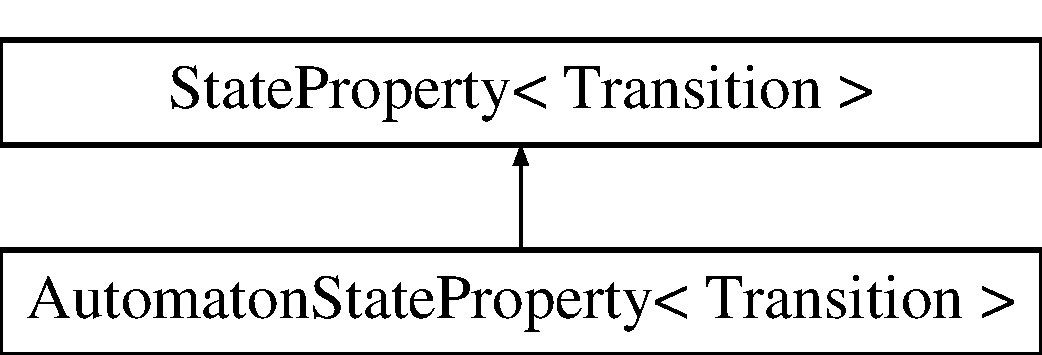
\includegraphics[height=2.000000cm]{structStateProperty}
\end{center}
\end{figure}
\subsection*{\-Public \-Member \-Functions}
\begin{DoxyCompactItemize}
\item 
\hyperlink{structStateProperty_ae35beca78b7de03eb461dfea8f55fccb}{\-State\-Property} (const \-State\-I\-D \-\_\-\-I\-D, const std\-::string \&\&\-\_\-label)
\end{DoxyCompactItemize}
\subsection*{\-Public \-Attributes}
\begin{DoxyCompactItemize}
\item 
\hypertarget{structStateProperty_af33be20c9033f9b6524c0447e7ac647e}{\-State\-I\-D \hyperlink{structStateProperty_af33be20c9033f9b6524c0447e7ac647e}{\-I\-D}}\label{structStateProperty_af33be20c9033f9b6524c0447e7ac647e}

\begin{DoxyCompactList}\small\item\em \-Unique \-I\-D of the state. \end{DoxyCompactList}\item 
\hypertarget{structStateProperty_a7cfb634f80b68196eefa54e8ee98a5fe}{std\-::string \hyperlink{structStateProperty_a7cfb634f80b68196eefa54e8ee98a5fe}{label}}\label{structStateProperty_a7cfb634f80b68196eefa54e8ee98a5fe}

\begin{DoxyCompactList}\small\item\em \-Label of the state (usually a number or series of numbers) descibing the state. \end{DoxyCompactList}\item 
\hypertarget{structStateProperty_a1bbac90e1ce9ff4f54749eaeff3847cb}{std\-::vector$<$ \-Transition $>$ \hyperlink{structStateProperty_a1bbac90e1ce9ff4f54749eaeff3847cb}{transitions}}\label{structStateProperty_a1bbac90e1ce9ff4f54749eaeff3847cb}

\begin{DoxyCompactList}\small\item\em \-Graph or automaton transitions, basically it is an edge with a label. \end{DoxyCompactList}\end{DoxyCompactItemize}
\subsubsection*{template$<$typename \-Transition$>$ struct State\-Property$<$ Transition $>$}



\subsection{\-Constructor \& \-Destructor \-Documentation}
\hypertarget{structStateProperty_ae35beca78b7de03eb461dfea8f55fccb}{\index{\-State\-Property@{\-State\-Property}!\-State\-Property@{\-State\-Property}}
\index{\-State\-Property@{\-State\-Property}!StateProperty@{\-State\-Property}}
\subsubsection[{\-State\-Property}]{\setlength{\rightskip}{0pt plus 5cm}template$<$typename \-Transition$>$ {\bf \-State\-Property}$<$ \-Transition $>$\-::{\bf \-State\-Property} (
\begin{DoxyParamCaption}
\item[{const \-State\-I\-D}]{\-\_\-\-I\-D, }
\item[{const std\-::string \&\&}]{\-\_\-label}
\end{DoxyParamCaption}
)\hspace{0.3cm}{\ttfamily  \mbox{[}inline\mbox{]}}}}\label{structStateProperty_ae35beca78b7de03eb461dfea8f55fccb}
\-Basic constructor that fills in the \-I\-D and label. 

\-The documentation for this struct was generated from the following file\-:\begin{DoxyCompactItemize}
\item 
construction/graph\-\_\-interface.\-hpp\end{DoxyCompactItemize}

\hypertarget{classSynthesisManager}{\section{\-Synthesis\-Manager \-Class \-Reference}
\label{classSynthesisManager}\index{\-Synthesis\-Manager@{\-Synthesis\-Manager}}
}


\-S\-T\-E\-P 3 -\/ \-Control class for the computation.  




{\ttfamily \#include $<$synthesis\-\_\-manager.\-hpp$>$}

\subsection*{\-Public \-Member \-Functions}
\begin{DoxyCompactItemize}
\item 
\hyperlink{classSynthesisManager_adad655ed16249bcfd9ac67afebfd507f}{\-Synthesis\-Manager} (const \hyperlink{classConstructionHolder}{\-Construction\-Holder} \&\-\_\-holder)
\item 
void \hyperlink{classSynthesisManager_a2ec413741cc5a8c1f4f96928abc71012}{do\-Synthesis} ()
\end{DoxyCompactItemize}


\subsection{\-Detailed \-Description}
\-Manager of the synthesis procedure -\/ takes the reference data constructed during previous steps and computes and executes the synthesis. \-Synthesis is done in three steps\-:
\begin{DoxyEnumerate}
\item preparation\-: empties data and starts a new round.
\end{DoxyEnumerate}

synthesis\-: computes the coloring, stored in the storage object and adds data to coloring analyzer if needed.
\begin{DoxyEnumerate}
\item conclusion\-: stores additional data and outputs 
\end{DoxyEnumerate}

\subsection{\-Constructor \& \-Destructor \-Documentation}
\hypertarget{classSynthesisManager_adad655ed16249bcfd9ac67afebfd507f}{\index{\-Synthesis\-Manager@{\-Synthesis\-Manager}!\-Synthesis\-Manager@{\-Synthesis\-Manager}}
\index{\-Synthesis\-Manager@{\-Synthesis\-Manager}!SynthesisManager@{\-Synthesis\-Manager}}
\subsubsection[{\-Synthesis\-Manager}]{\setlength{\rightskip}{0pt plus 5cm}\-Synthesis\-Manager\-::\-Synthesis\-Manager (
\begin{DoxyParamCaption}
\item[{const {\bf \-Construction\-Holder} \&}]{\-\_\-holder}
\end{DoxyParamCaption}
)\hspace{0.3cm}{\ttfamily  \mbox{[}inline\mbox{]}}}}\label{classSynthesisManager_adad655ed16249bcfd9ac67afebfd507f}
\-Constructor builds all the data objects that are used within. 

\subsection{\-Member \-Function \-Documentation}
\hypertarget{classSynthesisManager_a2ec413741cc5a8c1f4f96928abc71012}{\index{\-Synthesis\-Manager@{\-Synthesis\-Manager}!do\-Synthesis@{do\-Synthesis}}
\index{do\-Synthesis@{do\-Synthesis}!SynthesisManager@{\-Synthesis\-Manager}}
\subsubsection[{do\-Synthesis}]{\setlength{\rightskip}{0pt plus 5cm}void {\bf \-Synthesis\-Manager\-::do\-Synthesis} (
\begin{DoxyParamCaption}
{}
\end{DoxyParamCaption}
)\hspace{0.3cm}{\ttfamily  \mbox{[}inline\mbox{]}}}}\label{classSynthesisManager_a2ec413741cc5a8c1f4f96928abc71012}
\-Main synthesis function that iterates through all the rounds of the synthesis. 

\-The documentation for this class was generated from the following file\-:\begin{DoxyCompactItemize}
\item 
synthesis/synthesis\-\_\-manager.\-hpp\end{DoxyCompactItemize}

\hypertarget{classTimeManager}{\section{\-Time\-Manager \-Class \-Reference}
\label{classTimeManager}\index{\-Time\-Manager@{\-Time\-Manager}}
}


\-Class that allows to multiple clock for run-\/time measurement.  




{\ttfamily \#include $<$time\-\_\-manager.\-hpp$>$}

\subsection*{\-Public \-Member \-Functions}
\begin{DoxyCompactItemize}
\item 
void \hyperlink{classTimeManager_ac5210ba53dc521013e545ed5af34eab9}{start\-Clock} (const std\-::string clock\-\_\-name)
\item 
void \hyperlink{classTimeManager_ac9335bd758afc61eb6d935a9a0d3cbe5}{ouput\-Clock} (const std\-::string clock\-\_\-name) const 
\end{DoxyCompactItemize}


\subsection{\-Member \-Function \-Documentation}
\hypertarget{classTimeManager_ac9335bd758afc61eb6d935a9a0d3cbe5}{\index{\-Time\-Manager@{\-Time\-Manager}!ouput\-Clock@{ouput\-Clock}}
\index{ouput\-Clock@{ouput\-Clock}!TimeManager@{\-Time\-Manager}}
\subsubsection[{ouput\-Clock}]{\setlength{\rightskip}{0pt plus 5cm}void {\bf \-Time\-Manager\-::ouput\-Clock} (
\begin{DoxyParamCaption}
\item[{const std\-::string}]{clock\-\_\-name}
\end{DoxyParamCaption}
) const\hspace{0.3cm}{\ttfamily  \mbox{[}inline\mbox{]}}}}\label{classTimeManager_ac9335bd758afc61eb6d935a9a0d3cbe5}
\-Outputs current runtime of the clock.


\begin{DoxyParams}{\-Parameters}
{\em clock\-\_\-name} & name of the clock to output (also appears on the output) \\
\hline
\end{DoxyParams}
\hypertarget{classTimeManager_ac5210ba53dc521013e545ed5af34eab9}{\index{\-Time\-Manager@{\-Time\-Manager}!start\-Clock@{start\-Clock}}
\index{start\-Clock@{start\-Clock}!TimeManager@{\-Time\-Manager}}
\subsubsection[{start\-Clock}]{\setlength{\rightskip}{0pt plus 5cm}void {\bf \-Time\-Manager\-::start\-Clock} (
\begin{DoxyParamCaption}
\item[{const std\-::string}]{clock\-\_\-name}
\end{DoxyParamCaption}
)\hspace{0.3cm}{\ttfamily  \mbox{[}inline\mbox{]}}}}\label{classTimeManager_ac5210ba53dc521013e545ed5af34eab9}
\-Starts a clock with given name and, if it is requsted by user, outputs the info.


\begin{DoxyParams}{\-Parameters}
{\em clock\-\_\-name} & unique \-I\-D of the clock that will also be send on the output \\
\hline
\end{DoxyParams}


\-The documentation for this class was generated from the following file\-:\begin{DoxyCompactItemize}
\item 
auxiliary/time\-\_\-manager.\-hpp\end{DoxyCompactItemize}

\hypertarget{classTimeSeriesParser}{\section{\-Time\-Series\-Parser \-Class \-Reference}
\label{classTimeSeriesParser}\index{\-Time\-Series\-Parser@{\-Time\-Series\-Parser}}
}


\-This class parses takes the time series and builds it into a \-Buchi automaton.  




{\ttfamily \#include $<$time\-\_\-series\-\_\-parser.\-hpp$>$}

\subsection*{\-Public \-Member \-Functions}
\begin{DoxyCompactItemize}
\item 
\hypertarget{classTimeSeriesParser_a0d25ff75b9cd95200c9e63efa5d1aaa7}{\hyperlink{classTimeSeriesParser_a0d25ff75b9cd95200c9e63efa5d1aaa7}{\-Time\-Series\-Parser} (\hyperlink{classModel}{\-Model} \&\-\_\-model)}\label{classTimeSeriesParser_a0d25ff75b9cd95200c9e63efa5d1aaa7}

\begin{DoxyCompactList}\small\item\em \-Simple constructor, passes references. \end{DoxyCompactList}\item 
void \hyperlink{classTimeSeriesParser_a4c5a27d6f5df1595dff6264e511ec771}{parse} (const rapidxml\-::xml\-\_\-node$<$$>$ $\ast$const model\-\_\-node)
\end{DoxyCompactItemize}


\subsection{\-Member \-Function \-Documentation}
\hypertarget{classTimeSeriesParser_a4c5a27d6f5df1595dff6264e511ec771}{\index{\-Time\-Series\-Parser@{\-Time\-Series\-Parser}!parse@{parse}}
\index{parse@{parse}!TimeSeriesParser@{\-Time\-Series\-Parser}}
\subsubsection[{parse}]{\setlength{\rightskip}{0pt plus 5cm}void {\bf \-Time\-Series\-Parser\-::parse} (
\begin{DoxyParamCaption}
\item[{const rapidxml\-::xml\-\_\-node$<$$>$ $\ast$const}]{model\-\_\-node}
\end{DoxyParamCaption}
)\hspace{0.3cm}{\ttfamily  \mbox{[}inline\mbox{]}}}}\label{classTimeSeriesParser_a4c5a27d6f5df1595dff6264e511ec771}
\-Main parsing function. \-It expects a pointer to inside of a \-M\-O\-D\-E\-L node. 

\-The documentation for this class was generated from the following file\-:\begin{DoxyCompactItemize}
\item 
parsing/time\-\_\-series\-\_\-parser.\-hpp\end{DoxyCompactItemize}

\hypertarget{structTransitionProperty}{\section{\-Transition\-Property \-Struct \-Reference}
\label{structTransitionProperty}\index{\-Transition\-Property@{\-Transition\-Property}}
}


\-This is just a very simple basis for a transition in a graph.  




{\ttfamily \#include $<$graph\-\_\-interface.\-hpp$>$}

\-Inheritance diagram for \-Transition\-Property\-:\begin{figure}[H]
\begin{center}
\leavevmode
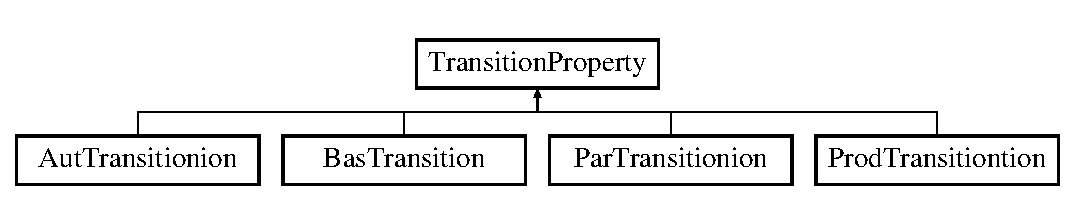
\includegraphics[height=2.000000cm]{structTransitionProperty}
\end{center}
\end{figure}
\subsection*{\-Public \-Member \-Functions}
\begin{DoxyCompactItemize}
\item 
\hyperlink{structTransitionProperty_a751d0faf12a55387f4a9680988401755}{\-Transition\-Property} (\-State\-I\-D \-\_\-target\-\_\-\-I\-D)
\end{DoxyCompactItemize}
\subsection*{\-Public \-Attributes}
\begin{DoxyCompactItemize}
\item 
\hypertarget{structTransitionProperty_a1e272cf5a26a0db442ac0fed5b797386}{\-State\-I\-D \hyperlink{structTransitionProperty_a1e272cf5a26a0db442ac0fed5b797386}{target\-\_\-\-I\-D}}\label{structTransitionProperty_a1e272cf5a26a0db442ac0fed5b797386}

\begin{DoxyCompactList}\small\item\em \-Unique \-I\-D of the state. \end{DoxyCompactList}\end{DoxyCompactItemize}


\subsection{\-Constructor \& \-Destructor \-Documentation}
\hypertarget{structTransitionProperty_a751d0faf12a55387f4a9680988401755}{\index{\-Transition\-Property@{\-Transition\-Property}!\-Transition\-Property@{\-Transition\-Property}}
\index{\-Transition\-Property@{\-Transition\-Property}!TransitionProperty@{\-Transition\-Property}}
\subsubsection[{\-Transition\-Property}]{\setlength{\rightskip}{0pt plus 5cm}{\bf \-Transition\-Property\-::\-Transition\-Property} (
\begin{DoxyParamCaption}
\item[{\-State\-I\-D}]{\-\_\-target\-\_\-\-I\-D}
\end{DoxyParamCaption}
)\hspace{0.3cm}{\ttfamily  \mbox{[}inline\mbox{]}}}}\label{structTransitionProperty_a751d0faf12a55387f4a9680988401755}
\-Basic constructor fills in the \-I\-D. 

\-The documentation for this struct was generated from the following file\-:\begin{DoxyCompactItemize}
\item 
construction/graph\-\_\-interface.\-hpp\end{DoxyCompactItemize}

\hypertarget{classUserOptions}{\section{\-User\-Options \-Class \-Reference}
\label{classUserOptions}\index{\-User\-Options@{\-User\-Options}}
}


\-Storage of options obtained from execution arguments.  




{\ttfamily \#include $<$user\-\_\-options.\-hpp$>$}

\subsection*{\-Public \-Member \-Functions}
\begin{DoxyCompactItemize}
\item 
\hyperlink{classUserOptions_a477c8d918c09c047e22fee763478b47e}{\-User\-Options} ()
\item 
bool \hyperlink{classUserOptions_abbcaaca086fb7d3bdd0868ad95800212}{robustness} () const 
\item 
bool \hyperlink{classUserOptions_a5620de91cbbd3787b8891a5eca7ea0d4}{witnesses} () const 
\item 
bool \hyperlink{classUserOptions_a3a05c437bb0193e05c97d6075a236002}{analysis} () const 
\item 
bool \hyperlink{classUserOptions_a43ea432ffbca6fc3c62afc8d3779fe30}{long\-Wit} () const 
\item 
bool \hyperlink{classUserOptions_a9f333311f79b960dba6e0955cb4fcd29}{verbose} () const 
\item 
bool \hyperlink{classUserOptions_a47ba8b52479f2fee0b8358b95fd9f10e}{stats} () const 
\item 
bool \hyperlink{classUserOptions_a66600767c4b6f6ab02ca66f59f074879}{time\-Series} () const 
\item 
std\-::size\-\_\-t \hyperlink{classUserOptions_a0c2e6be99071ffd34bfc326fcf0428c5}{proc\-Num} () const 
\item 
std\-::size\-\_\-t \hyperlink{classUserOptions_a7b7a9345c0f3df61e2ff7a488a5c717c}{proc\-Count} () const 
\item 
std\-::size\-\_\-t \hyperlink{classUserOptions_aa7d408830d57e58fe174b7e31242c435}{input\-Mask} () const 
\item 
std\-::size\-\_\-t \hyperlink{classUserOptions_a92e29f3823cec251841bcd14ad95079c}{output\-Mask} () const 
\end{DoxyCompactItemize}
\subsection*{\-Friends}
\begin{DoxyCompactItemize}
\item 
\hypertarget{classUserOptions_a55c9e1ac006a645af402e3aee6b64e00}{class {\bfseries \-Argument\-Parser}}\label{classUserOptions_a55c9e1ac006a645af402e3aee6b64e00}

\item 
\hypertarget{classUserOptions_a2759f637c8f028a9ed4256db41bf34ac}{class {\bfseries \-Model\-Parser}}\label{classUserOptions_a2759f637c8f028a9ed4256db41bf34ac}

\end{DoxyCompactItemize}


\subsection{\-Detailed \-Description}
\-Class that stores options provided by the user on the input. \-Values can be set up only using the \hyperlink{classArgumentParser}{\-Argument\-Parser} object. \-Further access to global object user\-\_\-options is possible only due to constant getters. \-Only a single object is intended to exist. 

\subsection{\-Constructor \& \-Destructor \-Documentation}
\hypertarget{classUserOptions_a477c8d918c09c047e22fee763478b47e}{\index{\-User\-Options@{\-User\-Options}!\-User\-Options@{\-User\-Options}}
\index{\-User\-Options@{\-User\-Options}!UserOptions@{\-User\-Options}}
\subsubsection[{\-User\-Options}]{\setlength{\rightskip}{0pt plus 5cm}\-User\-Options\-::\-User\-Options (
\begin{DoxyParamCaption}
{}
\end{DoxyParamCaption}
)\hspace{0.3cm}{\ttfamily  \mbox{[}inline\mbox{]}}}}\label{classUserOptions_a477c8d918c09c047e22fee763478b47e}
\-Constructor, sets up default values. 

\subsection{\-Member \-Function \-Documentation}
\hypertarget{classUserOptions_a3a05c437bb0193e05c97d6075a236002}{\index{\-User\-Options@{\-User\-Options}!analysis@{analysis}}
\index{analysis@{analysis}!UserOptions@{\-User\-Options}}
\subsubsection[{analysis}]{\setlength{\rightskip}{0pt plus 5cm}bool {\bf \-User\-Options\-::analysis} (
\begin{DoxyParamCaption}
{}
\end{DoxyParamCaption}
) const\hspace{0.3cm}{\ttfamily  \mbox{[}inline\mbox{]}}}}\label{classUserOptions_a3a05c437bb0193e05c97d6075a236002}
\begin{DoxyReturn}{\-Returns}
true if additional analysis will be computed (witnesses/robustness) 
\end{DoxyReturn}
\hypertarget{classUserOptions_aa7d408830d57e58fe174b7e31242c435}{\index{\-User\-Options@{\-User\-Options}!input\-Mask@{input\-Mask}}
\index{input\-Mask@{input\-Mask}!UserOptions@{\-User\-Options}}
\subsubsection[{input\-Mask}]{\setlength{\rightskip}{0pt plus 5cm}std\-::size\-\_\-t {\bf \-User\-Options\-::input\-Mask} (
\begin{DoxyParamCaption}
{}
\end{DoxyParamCaption}
) const\hspace{0.3cm}{\ttfamily  \mbox{[}inline\mbox{]}}}}\label{classUserOptions_aa7d408830d57e58fe174b7e31242c435}
\begin{DoxyReturn}{\-Returns}
true if the input mask was provided 
\end{DoxyReturn}
\hypertarget{classUserOptions_a43ea432ffbca6fc3c62afc8d3779fe30}{\index{\-User\-Options@{\-User\-Options}!long\-Wit@{long\-Wit}}
\index{long\-Wit@{long\-Wit}!UserOptions@{\-User\-Options}}
\subsubsection[{long\-Wit}]{\setlength{\rightskip}{0pt plus 5cm}bool {\bf \-User\-Options\-::long\-Wit} (
\begin{DoxyParamCaption}
{}
\end{DoxyParamCaption}
) const\hspace{0.3cm}{\ttfamily  \mbox{[}inline\mbox{]}}}}\label{classUserOptions_a43ea432ffbca6fc3c62afc8d3779fe30}
\begin{DoxyReturn}{\-Returns}
true if use\-\_\-long\-\_\-witnesses is set (display state levels instead of just a number) 
\end{DoxyReturn}
\hypertarget{classUserOptions_a92e29f3823cec251841bcd14ad95079c}{\index{\-User\-Options@{\-User\-Options}!output\-Mask@{output\-Mask}}
\index{output\-Mask@{output\-Mask}!UserOptions@{\-User\-Options}}
\subsubsection[{output\-Mask}]{\setlength{\rightskip}{0pt plus 5cm}std\-::size\-\_\-t {\bf \-User\-Options\-::output\-Mask} (
\begin{DoxyParamCaption}
{}
\end{DoxyParamCaption}
) const\hspace{0.3cm}{\ttfamily  \mbox{[}inline\mbox{]}}}}\label{classUserOptions_a92e29f3823cec251841bcd14ad95079c}
\begin{DoxyReturn}{\-Returns}
true if the mask of computation should be printed 
\end{DoxyReturn}
\hypertarget{classUserOptions_a7b7a9345c0f3df61e2ff7a488a5c717c}{\index{\-User\-Options@{\-User\-Options}!proc\-Count@{proc\-Count}}
\index{proc\-Count@{proc\-Count}!UserOptions@{\-User\-Options}}
\subsubsection[{proc\-Count}]{\setlength{\rightskip}{0pt plus 5cm}std\-::size\-\_\-t {\bf \-User\-Options\-::proc\-Count} (
\begin{DoxyParamCaption}
{}
\end{DoxyParamCaption}
) const\hspace{0.3cm}{\ttfamily  \mbox{[}inline\mbox{]}}}}\label{classUserOptions_a7b7a9345c0f3df61e2ff7a488a5c717c}
\begin{DoxyReturn}{\-Returns}
total number of processes in distributed computation 
\end{DoxyReturn}
\hypertarget{classUserOptions_a0c2e6be99071ffd34bfc326fcf0428c5}{\index{\-User\-Options@{\-User\-Options}!proc\-Num@{proc\-Num}}
\index{proc\-Num@{proc\-Num}!UserOptions@{\-User\-Options}}
\subsubsection[{proc\-Num}]{\setlength{\rightskip}{0pt plus 5cm}std\-::size\-\_\-t {\bf \-User\-Options\-::proc\-Num} (
\begin{DoxyParamCaption}
{}
\end{DoxyParamCaption}
) const\hspace{0.3cm}{\ttfamily  \mbox{[}inline\mbox{]}}}}\label{classUserOptions_a0c2e6be99071ffd34bfc326fcf0428c5}
\begin{DoxyReturn}{\-Returns}
number of this process in distributed computation (indexed from 1) 
\end{DoxyReturn}
\hypertarget{classUserOptions_abbcaaca086fb7d3bdd0868ad95800212}{\index{\-User\-Options@{\-User\-Options}!robustness@{robustness}}
\index{robustness@{robustness}!UserOptions@{\-User\-Options}}
\subsubsection[{robustness}]{\setlength{\rightskip}{0pt plus 5cm}bool {\bf \-User\-Options\-::robustness} (
\begin{DoxyParamCaption}
{}
\end{DoxyParamCaption}
) const\hspace{0.3cm}{\ttfamily  \mbox{[}inline\mbox{]}}}}\label{classUserOptions_abbcaaca086fb7d3bdd0868ad95800212}
\begin{DoxyReturn}{\-Returns}
true if compute\-\_\-robustness (robustness output is requested) 
\end{DoxyReturn}
\hypertarget{classUserOptions_a47ba8b52479f2fee0b8358b95fd9f10e}{\index{\-User\-Options@{\-User\-Options}!stats@{stats}}
\index{stats@{stats}!UserOptions@{\-User\-Options}}
\subsubsection[{stats}]{\setlength{\rightskip}{0pt plus 5cm}bool {\bf \-User\-Options\-::stats} (
\begin{DoxyParamCaption}
{}
\end{DoxyParamCaption}
) const\hspace{0.3cm}{\ttfamily  \mbox{[}inline\mbox{]}}}}\label{classUserOptions_a47ba8b52479f2fee0b8358b95fd9f10e}
\begin{DoxyReturn}{\-Returns}
true if display\-\_\-stats is set (displaying statistics of the model) 
\end{DoxyReturn}
\hypertarget{classUserOptions_a66600767c4b6f6ab02ca66f59f074879}{\index{\-User\-Options@{\-User\-Options}!time\-Series@{time\-Series}}
\index{time\-Series@{time\-Series}!UserOptions@{\-User\-Options}}
\subsubsection[{time\-Series}]{\setlength{\rightskip}{0pt plus 5cm}bool {\bf \-User\-Options\-::time\-Series} (
\begin{DoxyParamCaption}
{}
\end{DoxyParamCaption}
) const\hspace{0.3cm}{\ttfamily  \mbox{[}inline\mbox{]}}}}\label{classUserOptions_a66600767c4b6f6ab02ca66f59f074879}
\begin{DoxyReturn}{\-Returns}
true if property is a time series 
\end{DoxyReturn}
\hypertarget{classUserOptions_a9f333311f79b960dba6e0955cb4fcd29}{\index{\-User\-Options@{\-User\-Options}!verbose@{verbose}}
\index{verbose@{verbose}!UserOptions@{\-User\-Options}}
\subsubsection[{verbose}]{\setlength{\rightskip}{0pt plus 5cm}bool {\bf \-User\-Options\-::verbose} (
\begin{DoxyParamCaption}
{}
\end{DoxyParamCaption}
) const\hspace{0.3cm}{\ttfamily  \mbox{[}inline\mbox{]}}}}\label{classUserOptions_a9f333311f79b960dba6e0955cb4fcd29}
\begin{DoxyReturn}{\-Returns}
true if verbose is set (displaying additional information during computation) 
\end{DoxyReturn}
\hypertarget{classUserOptions_a5620de91cbbd3787b8891a5eca7ea0d4}{\index{\-User\-Options@{\-User\-Options}!witnesses@{witnesses}}
\index{witnesses@{witnesses}!UserOptions@{\-User\-Options}}
\subsubsection[{witnesses}]{\setlength{\rightskip}{0pt plus 5cm}bool {\bf \-User\-Options\-::witnesses} (
\begin{DoxyParamCaption}
{}
\end{DoxyParamCaption}
) const\hspace{0.3cm}{\ttfamily  \mbox{[}inline\mbox{]}}}}\label{classUserOptions_a5620de91cbbd3787b8891a5eca7ea0d4}
\begin{DoxyReturn}{\-Returns}
true if witnesses are to be computed 
\end{DoxyReturn}


\-The documentation for this class was generated from the following file\-:\begin{DoxyCompactItemize}
\item 
auxiliary/user\-\_\-options.\-hpp\end{DoxyCompactItemize}

\hypertarget{classWitnessSearcher}{\section{\-Witness\-Searcher \-Class \-Reference}
\label{classWitnessSearcher}\index{\-Witness\-Searcher@{\-Witness\-Searcher}}
}


\-Class for search of transitions belonging to shortest time series paths.  




{\ttfamily \#include $<$witness\-\_\-searcher.\-hpp$>$}

\subsection*{\-Classes}
\begin{DoxyCompactItemize}
\item 
struct {\bfseries \-Marking}
\begin{DoxyCompactList}\small\item\em \-This structure stores \char`\"{}already tested\char`\"{} paramsets for a state. \end{DoxyCompactList}\end{DoxyCompactItemize}
\subsection*{\-Public \-Member \-Functions}
\begin{DoxyCompactItemize}
\item 
\hyperlink{classWitnessSearcher_ad228f655ca01b5edecb2245218cd123f}{\-Witness\-Searcher} (const \hyperlink{classConstructionHolder}{\-Construction\-Holder} \&\-\_\-holder, const \hyperlink{classColorStorage}{\-Color\-Storage} \&\-\_\-storage)
\item 
void \hyperlink{classWitnessSearcher_a2d1153ac29c1e1ad653798564a067e29}{find\-Witnesses} ()
\item 
const std\-::vector$<$ std\-::string $>$ \hyperlink{classWitnessSearcher_a00d963143076bbb09f12c361f814f24f}{get\-Output} () const 
\item 
const std\-::vector$<$ std\-::set\*
$<$ std\-::pair$<$ \-State\-I\-D, \-State\-I\-D $>$ $>$ $>$ \& \hyperlink{classWitnessSearcher_a58a37b8190683b9adf5eaf5a4c9b3e68}{get\-Transitions} () const 
\item 
const std\-::vector$<$ std\-::set\*
$<$ \-State\-I\-D $>$ $>$ \& \hyperlink{classWitnessSearcher_a4d2540526995ff077c33c6a62670a047}{get\-Initials} () const 
\end{DoxyCompactItemize}


\subsection{\-Detailed \-Description}
\-Class executes a search through the synthetized space in order to find transitions included in shortest paths for every parametrization. \-Procedure is supposed to be first executed and then it can provide results. 

\subsection{\-Constructor \& \-Destructor \-Documentation}
\hypertarget{classWitnessSearcher_ad228f655ca01b5edecb2245218cd123f}{\index{\-Witness\-Searcher@{\-Witness\-Searcher}!\-Witness\-Searcher@{\-Witness\-Searcher}}
\index{\-Witness\-Searcher@{\-Witness\-Searcher}!WitnessSearcher@{\-Witness\-Searcher}}
\subsubsection[{\-Witness\-Searcher}]{\setlength{\rightskip}{0pt plus 5cm}\-Witness\-Searcher\-::\-Witness\-Searcher (
\begin{DoxyParamCaption}
\item[{const {\bf \-Construction\-Holder} \&}]{\-\_\-holder, }
\item[{const {\bf \-Color\-Storage} \&}]{\-\_\-storage}
\end{DoxyParamCaption}
)\hspace{0.3cm}{\ttfamily  \mbox{[}inline\mbox{]}}}}\label{classWitnessSearcher_ad228f655ca01b5edecb2245218cd123f}
\-Constructor ensures that data objects used within the whole computation process have appropriate size. 

\subsection{\-Member \-Function \-Documentation}
\hypertarget{classWitnessSearcher_a2d1153ac29c1e1ad653798564a067e29}{\index{\-Witness\-Searcher@{\-Witness\-Searcher}!find\-Witnesses@{find\-Witnesses}}
\index{find\-Witnesses@{find\-Witnesses}!WitnessSearcher@{\-Witness\-Searcher}}
\subsubsection[{find\-Witnesses}]{\setlength{\rightskip}{0pt plus 5cm}void {\bf \-Witness\-Searcher\-::find\-Witnesses} (
\begin{DoxyParamCaption}
{}
\end{DoxyParamCaption}
)\hspace{0.3cm}{\ttfamily  \mbox{[}inline\mbox{]}}}}\label{classWitnessSearcher_a2d1153ac29c1e1ad653798564a067e29}
\-Function that executes the whole searching process \hypertarget{classWitnessSearcher_a4d2540526995ff077c33c6a62670a047}{\index{\-Witness\-Searcher@{\-Witness\-Searcher}!get\-Initials@{get\-Initials}}
\index{get\-Initials@{get\-Initials}!WitnessSearcher@{\-Witness\-Searcher}}
\subsubsection[{get\-Initials}]{\setlength{\rightskip}{0pt plus 5cm}const std\-::vector$<$std\-::set$<$\-State\-I\-D$>$ $>$\& {\bf \-Witness\-Searcher\-::get\-Initials} (
\begin{DoxyParamCaption}
{}
\end{DoxyParamCaption}
) const\hspace{0.3cm}{\ttfamily  \mbox{[}inline\mbox{]}}}}\label{classWitnessSearcher_a4d2540526995ff077c33c6a62670a047}
\begin{DoxyReturn}{\-Returns}
a vector of \-I\-Ds of intial states 
\end{DoxyReturn}
\hypertarget{classWitnessSearcher_a00d963143076bbb09f12c361f814f24f}{\index{\-Witness\-Searcher@{\-Witness\-Searcher}!get\-Output@{get\-Output}}
\index{get\-Output@{get\-Output}!WitnessSearcher@{\-Witness\-Searcher}}
\subsubsection[{get\-Output}]{\setlength{\rightskip}{0pt plus 5cm}const std\-::vector$<$std\-::string$>$ {\bf \-Witness\-Searcher\-::get\-Output} (
\begin{DoxyParamCaption}
{}
\end{DoxyParamCaption}
) const\hspace{0.3cm}{\ttfamily  \mbox{[}inline\mbox{]}}}}\label{classWitnessSearcher_a00d963143076bbb09f12c361f814f24f}
\-Re-\/formes the transitions computed during the round into strings.

\begin{DoxyReturn}{\-Returns}
strings with all transitions for each acceptable parametrization 
\end{DoxyReturn}
\hypertarget{classWitnessSearcher_a58a37b8190683b9adf5eaf5a4c9b3e68}{\index{\-Witness\-Searcher@{\-Witness\-Searcher}!get\-Transitions@{get\-Transitions}}
\index{get\-Transitions@{get\-Transitions}!WitnessSearcher@{\-Witness\-Searcher}}
\subsubsection[{get\-Transitions}]{\setlength{\rightskip}{0pt plus 5cm}const std\-::vector$<$std\-::set$<$std\-::pair$<$\-State\-I\-D, \-State\-I\-D$>$ $>$ $>$\& {\bf \-Witness\-Searcher\-::get\-Transitions} (
\begin{DoxyParamCaption}
{}
\end{DoxyParamCaption}
) const\hspace{0.3cm}{\ttfamily  \mbox{[}inline\mbox{]}}}}\label{classWitnessSearcher_a58a37b8190683b9adf5eaf5a4c9b3e68}
\begin{DoxyReturn}{\-Returns}
transitions for each parametrizations in the form (source, target) 
\end{DoxyReturn}


\-The documentation for this class was generated from the following file\-:\begin{DoxyCompactItemize}
\item 
synthesis/witness\-\_\-searcher.\-hpp\end{DoxyCompactItemize}

\printindex
\end{document}
